\documentclass[12pt,a4paper,openright,twoside]{report}

\usepackage[T1]{fontenc}   
\usepackage[utf8]{inputenc}
\usepackage[a4paper]{geometry}
\usepackage{fancyhdr}
\usepackage{graphicx}
\usepackage[pdfpagelabels]{hyperref}
\usepackage{amsthm, amsmath, amssymb, mathtools}
\usepackage{listings}
\usepackage{booktabs}
\usepackage{parskip} 
\usepackage{array}
\usepackage[italian]{babel}
\usepackage{siunitx}
\usepackage[table]{xcolor}

\newtheorem{theorem}{Teorema}

\linespread{1.2}
\raggedbottom{} % Non forzare il contenuto a riempire la pagina
\setlength{\intextsep}{20pt}   % Spazio sopra e sotto le figure posizionate con [h] o [H]

% Configurazione Intestazioni
\pagestyle{fancy}
\renewcommand{\chaptermark}[1]{\markboth{\thechapter.\ #1}{}}
\renewcommand{\sectionmark}[1]{\markright{\thesection{} \ #1}{}}
\rhead[\fancyplain{}{\bfseries\leftmark}]{\fancyplain{}{\bfseries\thepage}}
\lhead[\fancyplain{}{\bfseries\thepage}]{\fancyplain{}{\bfseries\rightmark}}
\cfoot{}



\begin{document}
%------------FRONTESPIZIO------------------
\begin{titlepage}
% Forziamo margini simmetrici e textwidth a 450pt per il frontespizio
\newgeometry{left=75pt, right=75pt, top=2cm, bottom=2.5cm}
% OLD: \newgeometry{left=72pt, right=72pt, top=2cm, bottom=2cm}
\setlength{\textwidth}{450pt}

\begin{center}
    
\includegraphics[width=0.25\linewidth]{images/logo_unibo.png}\vspace{0.7cm}\\

    {{\Large{\textsc{Alma Mater Studiorum $\cdot$ Universit\`a di Bologna}}}} \\
    \rule[0.1cm]{15.8cm}{0.1mm}
    \rule[0.5cm]{15.8cm}{0.6mm}

    {\small{\bf DIPARTIMENTO DI INFORMATICA --- SCIENZA E INGEGNERIA\\
    Corso di Laurea in Ingegneria e Scienze Informatiche}}
\end{center}

\vfill

\begin{center}
    {\LARGE{\bf
        \linespread{1}\selectfont
        Sviluppo di un modello di Deep Learning per il rilevamento del malposizionamento degli elettrodi in un ECG a 12 derivazioni\par
    }}
    \vspace{19mm}
    {\large{\bf Tesi di Laurea in Metodi Numerici}}
\end{center}

\vfill

\par
\noindent
\begin{minipage}[t]{0.50\textwidth}
    {\large\bf Relatrice:}\\[1mm]
    {\large\bf Prof.ssa Damiana Lazzaro}\\[5mm]
    {\large\bf Correlatore:}\\[1mm]
    {\large\bf Prof. Johannes De Bie}
\end{minipage}
\hfill
\begin{minipage}[t]{0.47\textwidth}\raggedleft{}
    {\large{\bf Presentata da:\\[1mm]
    Nicholas Benedetti}}
\end{minipage}

\vfill

\begin{center}
    {\large{\bf Sessione Unica\\}}
    {\large{\bf Anno Accademico 2025/2026}}
\end{center}
\end{titlepage}
\pagestyle{empty}
%------------FRONTESPIZIO------------------

\tableofcontents

% Margini classici: 3.5cm sopra/sotto e 3cm ai lati + rilegatura
\newgeometry{
    lines=33,
    includehead,
    vmarginratio=1:1, % Centra verticalmente il blocco delle 33 righe
    bindingoffset=7mm, % Spazio per la rilegatura
    inner=35mm,       % Margine interno (lato rilegatura)
    outer=35mm        % Margine esterno
}

%Per la riga di intestazione
\setlength{\headwidth}{\textwidth}
\addtolength{\headwidth}{20pt} % Circa 7 mm

\pagenumbering{arabic}
\pagestyle{plain}
%---------------CAPITOLO 1---------------
\chapter{Introduzione}

\section{Il problema del malposizionamento degli elettrodi}

L'elettrocardiogramma a 12 derivazioni è, ancora oggi, lo strumento diagnostico più diffuso ed economico per la valutazione dell'attività elettrica del cuore, ed è alla base della diagnosi di un ampio spettro di patologie cardiovascolari. La sua affidabilità clinica dipende però in modo critico dalla corretta esecuzione del posizionamento dei dieci elettrodi sulla superficie corporea del paziente, secondo lo standard descritto nella sezione \ref{pos_elettrodi}.

Nella pratica clinica quotidiana, questo posizionamento non è sempre eseguito correttamente. Lo scambio di due elettrodi periferici (ad esempio: braccio destro e braccio sinistro) o il posizionamento non corretto di uno o più elettrodi precordiali sono errori tutt'altro che rari: la letteratura riporta un'incidenza di malposizionamento che, a seconda del contesto di acquisizione e della tipologia di errore considerata, varia indicativamente da meno dell'1\% fino a diversi punti percentuali dei tracciati registrati. Il problema però, è molto più subdolo: un elettrodo scambiato può alterare in modo sostanziale la morfologia delle onde P, del complesso QRS e dell'onda T, fino a simulare quadri patologici inesistenti (ad esempio un infarto anteriore o un pattern di tipo Brugada) oppure, viceversa, a mascherare un'alterazione realmente presente. Le conseguenze cliniche di una diagnosi errata derivante da un tracciato mal acquisito possono essere significative, sia in termini di sicurezza del paziente sia in termini di costi sanitari legati ad accertamenti diagnostici superflui.

A differenza di altri artefatti che affliggono il segnale ECG (rumore da rete elettrica, interferenza muscolare, movimento del paziente), il malposizionamento degli elettrodi produce un tracciato che, salvo casi particolari, resta \textit{"plausibile"}: le onde sono presenti, hanno un'ampiezza e una forma ragionevoli, e nulla nell'aspetto generale del tracciato segnala immediatamente l'anomalia a un occhio poco esperto. Questo rende il problema particolarmente insidioso e, al tempo stesso, difficile da affrontare con semplici tecniche di controllo qualità del segnale.

\section{Obiettivi della tesi}

L'obiettivo di questo lavoro è lo sviluppo e la validazione di un sistema automatico in grado di rilevare il malposizionamento degli elettrodi a partire da un singolo tracciato ECG a 12 derivazioni, senza richiedere un tracciato di riferimento acquisito correttamente sullo stesso paziente. In particolare, il lavoro si pone i seguenti obiettivi specifici:

\begin{itemize}
    \item costruire un dataset di grandi dimensioni ed etichettato in modo affidabile, a partire da database pubblici di ECG correttamente acquisiti, tramite la simulazione algebrica degli effetti di uno scambio di elettrodi sulle derivazioni standard;
    \item progettare un'architettura di deep learning in grado di sfruttare non solo l'informazione morfologica di ciascuna singola derivazione, ma anche la relazione \emph{spaziale} e \emph{temporale} che lega le diverse derivazioni tra loro;
    \item validare sperimentalmente il modello proposto su un insieme di test bilanciato, misurandone le prestazioni complessive e per singola tipologia di scambio, e confrontandole con approcci di riferimento più semplici;
    \item discutere criticamente i risultati ottenuti, i limiti dell'approccio e la sua trasferibilità a un contesto clinico reale.
\end{itemize}

\section{Contributi della tesi}

Il contributo originale di questo lavoro può essere sintetizzato in tre punti principali.

In primo luogo, viene proposta una \textbf{pipeline di simulazione degli scambi di elettrodi} basata sulle equazioni algebriche che legano le derivazioni standard ai potenziali dei singoli elettrodi (leggi di Einthoven e Goldberger, terminale centrale di Wilson). Questo approccio consente di generare, a partire da tracciati acquisiti correttamente, esempi etichettati e realistici delle principali tipologie di scambio, superando l'assenza di annotazioni di questo tipo nei database pubblici disponibili.

In secondo luogo, vengono proposte tre architetture: una ibrida \emph{CNN+GCN}, in cui il ramo convoluzionale 1D estrae feature morfologiche da ciascuna derivazione, mentre la rete convoluzionale a grafo (\textit{Graph Convolutional Network}) mette in relazione tali feature secondo una matrice di adiacenza costruita a partire dalla geometria spaziale reale delle derivazioni; una \emph{CNN} pura e un \emph{MLP}.

In terzo luogo, viene condotta una \textbf{validazione sperimentale} del modello proposto, con un'analisi dei modelli allenati sulle stesse classi di scambio, anche multi-classe, e uno studio mirato all'identificazione dei malposizionamenti sfruttando falsi positivi e falsi negativi.

\section{Organizzazione dell'elaborato}

Il resto dell'elaborato è organizzato come segue.

Il Capitolo~2 richiama le nozioni di anatomia ed elettrofisiologia cardiaca necessarie a comprendere l'origine del segnale ECG, il posizionamento standard degli elettrodi, il calcolo delle dodici derivazioni e i criteri di normalità di un tracciato.

Il Capitolo~3 presenta una rassegna dello stato dell'arte relativo al rilevamento automatico del malposizionamento degli elettrodi, distinguendo tra metodi classici basati su regole cliniche e criteri morfologici e i più recenti approcci basati su machine learning e deep learning.

Il Capitolo~4 introduce le basi matematiche utilizzate nel resto del lavoro: le trasformate di Fourier, Laplace e Z, la teoria dei filtri lineari, e le tecniche di elaborazione del segnale ECG digitale (campionamento, quantizzazione, preprocessing e filtraggio).

Il Capitolo~5 descrive nel dettaglio la costruzione del dataset utilizzato, a partire dai database pubblici PTB-XL e Georgia, illustrando lo split per paziente, la segmentazione beat-by-beat e le equazioni utilizzate per simulare gli scambi di elettrodi.

Il Capitolo~6 descrive le architetture citate precedentemente e come avviene il \emph{message-passing} tra le varie architetture.

Il Capitolo~7 presenta il protocollo di validazione sperimentale, le metriche utilizzate e i risultati ottenuti, complessivi e per singola classe di scambio, confrontati con le baseline di riferimento.

Il Capitolo~8 discute i risultati ottenuti, analizzando le classi di scambio da identificare, la trasferibilità clinica del sistema e i limiti legati all'utilizzo di un dataset sintetico.

Il Capitolo~9, infine, riassume i risultati raggiunti e propone possibili sviluppi futuri del lavoro di ricerca.

%---------------CAPITOLO 1---------------

%---------------CAPITOLO 2---------------
\chapter{Elettrocardiografia e basi elettrofisiologiche}

\section{Anatomia ed elettrofisiologia del Cuore}
Il cuore è un organo muscolare cavo situato nel mediastino, leggermente spostato a sinistra. Ha il compito di distribuire il sangue (ossigenato e non) in tutto il nostro corpo.

Il cuore è diviso in quattro camere principali: atrio destro e sinistro, ventricolo destro e sinistro; gli atri sono posti nella parte superiore e hanno il compito di raccogliere il sangue e pomparlo dentro i ventricoli, questi ultimi sono le cavità più grandi e hanno il compito di pompare il sangue ognuno nelle proprie circolazioni: circolazione polmonare per il ventricolo destro e circolazione sistemica per il ventricolo sinistro.

\begin{center}
\begin{tabular}{>{\bfseries}l l l}
\toprule
Camera & Funzione & Vasi associati \\
\midrule
Atrio destro   & Raccoglie il sangue venoso sistemico  & Vene cave superiore e inferiore \\
Ventricolo destro & Pompa il sangue verso i polmoni    & Arteria polmonare \\
Atrio sinistro & Raccoglie il sangue ossigenato        & Vene polmonari \\
Ventricolo sinistro & Pompa il sangue verso il corpo   & Aorta \\
\bottomrule
\end{tabular}
\end{center}  
\begin{figure}[h!]
    \centering
    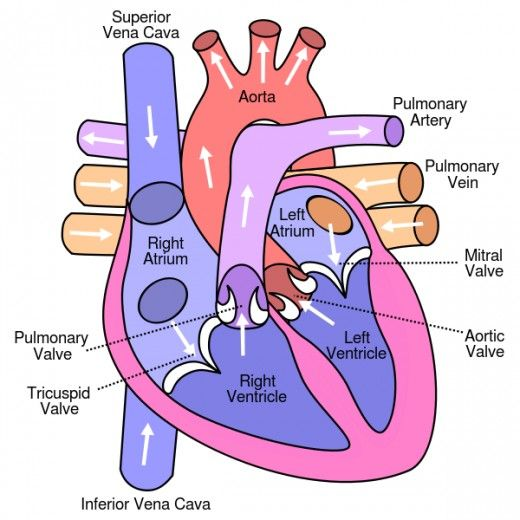
\includegraphics[width=0.6\linewidth]{images/heart.jpg}
    \caption{Foto del cuore con vene e arterie principali, presenti anche le valvole atrioventricolari e semilunari}
    \label{fig:placeholder}
\end{figure}
In ogni punto di comunicazione all'interno del cuore sono presenti delle valvole; esse garantiscono il flusso unidirezionale del sangue impedendone il reflusso. Le valvole si distinguono in due gruppi funzionali:

\begin{itemize}
  \item \textbf{Valvole atrioventricolari: (VA)} ancorate ai muscoli papillari del ventricolo tramite le \textit{corde tendinee}, che impediscono il prolasso dei lembi durante la sistole ventricolare; sono presenti due valvole di questo tipo: la \textit{valvola tricuspide}, posta tra atrio e ventricolo destro, è composta da tre lembi, e la \textit{valvola mitrale} (o bicuspide), posta tra tra atrio e ventricolo sinistro e composta da due lembi. 
  \item \textbf{Valvole semilunari:} prive di corde tendinee, si aprono e chiudono passivamente in risposta al gradiente di pressione. Abbiamo la \textit{valvola semilunare polmonare}, posta tra ventricolo destro e arteria polmonare, e la \textit{valvola semilunare aortica}, posta tra ventricolo sinistro e aorta.
\end{itemize}

\subsection{La parete cardiaca}

La parete del cuore è costituita da tre strati concentrici:
\begin{itemize}
  \item \textbf{Endocardio}: lo strato più interno, formato da tessuto endoteliale; riveste le cavità cardiache e le valvole.
  \item \textbf{Miocardio}: lo strato intermedio e più spesso, composto da cellule muscolari striate di tipo cardiaco (\textit{cardiomiociti}); è responsabile della forza contrattile del cuore. Lo spessore varia a seconda della camera: è massimo nel ventricolo sinistro, che deve vincere la resistenza della circolazione sistemica.
  \item \textbf{Epicardio}: lo strato più esterno, costituito da mesotelio e tessuto connettivo; corrisponde al \textit{foglietto viscerale} del pericardio sieroso.
\end{itemize}

Il cuore è poi avvolto esternamente dal \textbf{pericardio}, una sacca a doppia parete composta da:

\begin{itemize}
  \item \textbf{Pericardio fibroso}: lo strato esterno, robusto e inestensibile, che ancora il cuore al mediastino e lo protegge da sovradistensioni.
  \item \textbf{Pericardio sieroso}: suddiviso a sua volta in:\textit{Foglietto parietale} che riveste internamente il pericardio fibroso e il \textit{Foglietto viscerale} (o epicardio) che aderisce direttamente alla parete cardiaca.
\end{itemize}

Tra i due foglietti del pericardio sieroso è presente la \textbf{cavità pericardica}, che contiene una piccola quantità di liquido sieroso ($\sim$20--50 mL) con funzione lubrificante, riducendo l'attrito durante i movimenti del cuore.

\subsection{Contrazione e composizione cellulare}
Il cuore è composto principalmente da \textbf{cardiomiociti}, cellule 
muscolari striate specializzate che si contraggono involontariamente 
per pompare il sangue. Queste cellule sono connesse tramite i 
\textbf{dischi intercalari}, strutture che contengono desmosomi, 
utilizzati per l'ancoraggio meccanico, e \textbf{giunzioni gap}, canali che 
permettono il passaggio diretto di ioni tra cellule adiacenti, 
garantendo una propagazione rapida dell'impulso elettrico.
\begin{figure}[h!]
    \centering
    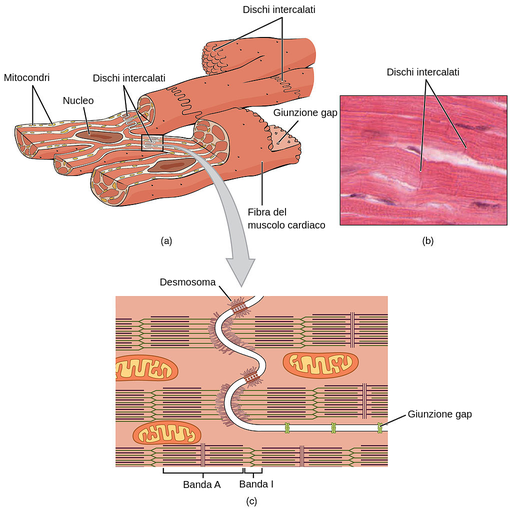
\includegraphics[width=0.33\linewidth]{images/cardiomicito.png}
    \caption{cardiomicito}
    \label{fig:cardiomicito}
\end{figure}

L'impulso viene generato dalle \textbf{cellule nodali}, in gergo \textit{pacemaker}, che a differenza dei cardiomiociti non si contraggono, ma sono specializzate nella generazione del segnale elettrico. Queste cellule sono raggruppate nell'atrio destro in prossimità della vena cava superiore, nel \textbf{nodo senoatriale (SA)}, e hanno la capacità di depolarizzarsi spontaneamente e ritmicamente, dando origine a ogni battito cardiaco. L'impulso generato viene poi irradiato in tutto il cuore tramite un sistema di conduzione composto da fibre di conduzione.
\begin{figure}[h!]
    \centering
    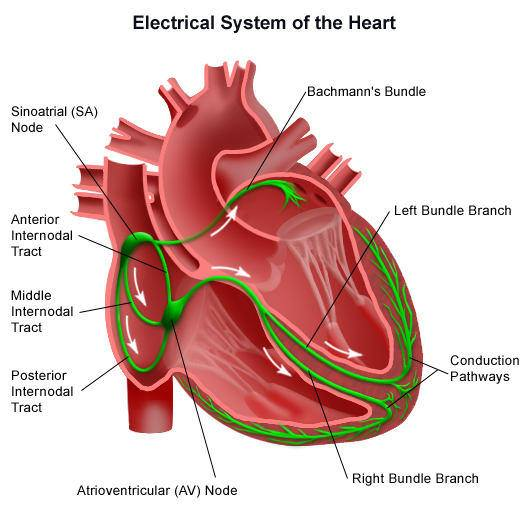
\includegraphics[width=0.3\linewidth]{images/sistema-elettrico-del-cuore.jpg}
    \caption{sistema di conduzione del cuore}
    \label{fig:sist-cond-cuore}
\end{figure}

\subsection{Il Ciclo Cardiaco}

Il ciclo cardiaco rappresenta la sequenza di eventi meccanici ed elettrici che si ripete ad ogni battito. A riposo, per un adulto medio, la frequenza cardiaca è di circa \textbf{60--80 battiti/min}, per cui ogni ciclo dura circa \textbf{800\,ms}. Ogni ciclo cardiaco è formato da due azioni principali: sistole (contrazione) e diastole (rilassamento).

\subsubsection{Prima fase}
La prima fase del ciclo cardiaco è per convenzione la \textbf{sistole atriale}, che spinge il sangue dagli atri nei ventricoli. Questa fase ha una durata di circa 100 ms, alla fine della quale, inizia la \textbf{diastole atriale} che durerà fino all'inizio del prossimo ciclo cardiaco.

\subsubsection{Seconda fase}
La seconda fase è invece la \textbf{sistole ventricolare}, questa ha una durata di circa 270 ms e suddivide ulteriormente in due sotto-fasi: 
\begin{itemize}
    \item \textbf{fase isovolumetrica}: dove la pressione spinge le valvole AV a chiudersi, ma non ne crea abbastanza per aprire le valvole semilunari.
    \item \textbf{fase propulsiva}: la pressione aumenta e supera quella delle arterie, le valvole semilunari si aprono e il sangue viene espulso.
\end{itemize}

\subsubsection{Terza fase}
Qui avviene l'ultima fase del ciclo cardiaco, la \textbf{diastole ventricolare}; anch'essa divisa in due sotto-fasi:
\begin{itemize}
    \item \textbf{fase precoce}: la pressione ventricolare inizia a calare, parte del sangue refluisce verso le valvole semilunari, chiudendole. Il sangue inizia a fluire negli atri rilasciati.
    \item \textbf{fase tardiva}: la diminuzione della pressione nei ventricoli apre le valvole AV, permettendo un riempimento passivo dei ventricoli.
\end{itemize}

\subsection{Elettrofisiologia}
Lo standard per l'elettrocardiogramma (ECG) è a dodici derivazioni, esse sono generate da 10 elettrodi posizionati sulla cute in specifici punti; prima di parlare di ECG, andiamo a vedere che cosa misuriamo effettivamenti tramite gli elettrodi.

\subsubsection{Potenziale di membrana}

I cardiomiociti, come tutte le cellule muscolari, mantengono a riposo un \textbf{potenziale di membrana negativo}, pari a circa \textbf{-90\,mV}; ed è proprio grazie a questo squilibrio elettrico che la cellula è in grado di contrarsi. Il potenziale negativo a riposo rappresenta infatti uno \textit{stato di carica}, come un condensatore pronto a scaricarsi: quando arriva il segnale elettrico appropriato, la cellula può depolarizzarsi rapidamente e innescare la contrazione muscolare.

\begin{figure}[h!]
    \centering
    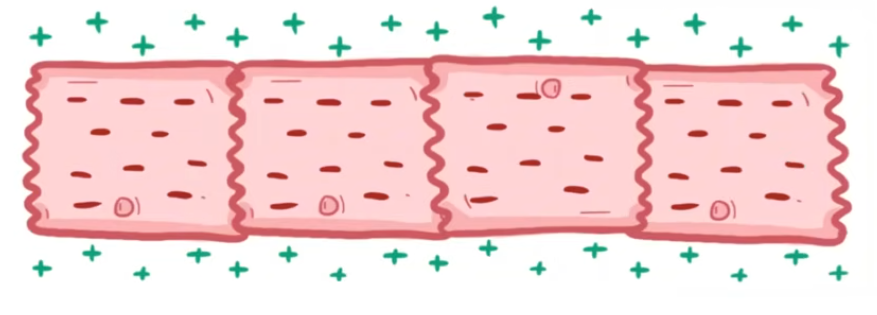
\includegraphics[width=0.4\linewidth]{images/potenziale-riposo-cardiomicito.png}
    \caption{Potenziale a riposo di un cardiomiocito}
    \label{fig:placeholder}
\end{figure}

Questo potenziale negativo viene mantenuto dalla naturale distribuzione asimmetrica degli ioni tra l'interno e l'esterno della cellula: gli ioni $K^+$ sono presenti in alta concentrazione \textit{all'interno}, mentre gli ioni $Na^+$ si trovano in alta concentrazione \textit{all'esterno}. Questa asimmetria, tuttavia, tende naturalmente a degradarsi. 

Gli ioni $K^+$, seguendo il loro gradiente di concentrazione, fuoriescono dalla cellula attraverso un canale passivo chiamato \textbf{Kir} (canale a rettificazione interna). Poiché ogni ione $K^+$ che esce porta con sé una carica positiva, l'interno della cellula diventa progressivamente più negativo contribuendo al potenziale di riposo, ma impoverendo la cellula di $K^+$.Per contrastare questa perdita e mantenere stabile la distribuzione ionica, entra in gioco la \textbf{pompa Na/K-ATPasi}. Si tratta di una pompa \textit{attiva}, che consuma energia sotto forma di ATP, che lavora \textit{contro gradiente} trasportando simultaneamente:

\begin{itemize}
    \item \textbf{3 ioni $Na^+$} verso l'esterno,
    \item \textbf{2 ioni $K^+$} verso l'interno.
\end{itemize}

In questo modo, la pompa ripristina continuamente le concentrazioni ioniche, mantenendo l'interno ricco di $K^+$ e l'esterno ricco di $Na^+$ e con esse, il potenziale di membrana negativo che rende possibile la contrazione.

\subsubsection{Fasi della contrazione}
Quando arriva lo stimolo generato dalle cellule nodali, il cardiomiocita attraversa un ciclo elettrico suddiviso in cinque fasi (da 0 a 4).

\begin{description}
    \item[Fase 0 -- Depolarizzazione rapida] 
    Lo stimolo provoca l'apertura dei canali voltaggio-dipendenti del $Na^+$, una grande quantità di ioni $Na^+$ entra all'interno della cellula, portando cariche positive all'interno. Il potenziale di membrana passa rapidamente da $-90$ mV a circa $+30$ mV. Questo processo, in cui la cellula perde la sua polarità negativa interna, prende il nome di \textbf{depolarizzazione}.

    \item[Fase 1 -- Ripolarizzazione iniziale]
    I canali del $Na^+$ si inattivano e gli ioni $K^+$ iniziano a muoversi verso gradiente tramite i canali passivi \textbf{Kir}, la fuoriuscita provoca una breve e parziale ripolarizzazione della membrana.

    \item[Fase 2 -- Plateau]
    Si apre una corrente di ioni $Ca^{2+}$ attraverso i canali di tipo L, la cui carica positiva in entrata \textbf{bilancia} la fuoriuscita di $K^+$, mantenendo il potenziale di membrana su un valore pressoché stabile per circa 200 ms. Questa fase è fondamentale perché l'ingresso di $Ca^{2+}$ permetta la contrazione del cardiomiocita.

    \item[Fase 3 -- Ripolarizzazione rapida]
    I canali del $Ca^{2+}$ si chiudono mentre i canali del $K^+$ rimangono 
    aperti: la fuoriuscita massiva di $K^+$ riporta il potenziale di 
    membrana rapidamente verso i valori di riposo.

    \item[Fase 4 -- Riposo]
    Il potenziale di membrana si stabilizza a $-90$ mV. La pompa $Na$/$K$ ripristina attivamente le concentrazioni ioniche originali, facendo uscire i $Na^+$ e reintroducendo $K^+$. Il processo opposto alla depolarizzazione, ovvero il ripristino della polarità negativa interna, prende il nome di \textbf{ripolarizzazione}.

\end{description}

\begin{figure}[h!]
    \centering
    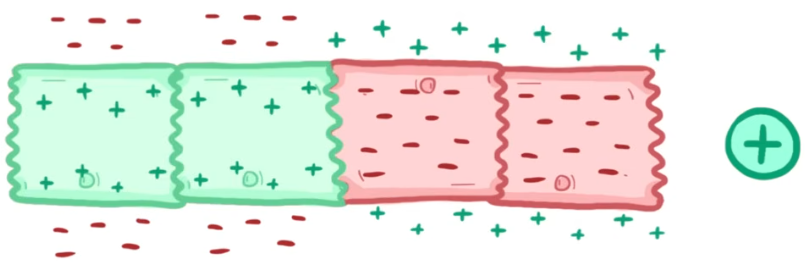
\includegraphics[width=0.4\linewidth]{images/onda-depolarizzazione.png}
    \caption{Onda di depolarizzazione, verso destra}
    \label{fig:placeholder}
\end{figure}

La cosa fondamentale è che la propagazione dello stimolo non avviene istantaneamente su tutte le cellule, ma si propaga nel tempo tramite le \textit{giunzioni gap}. Questa zona di confine tra la parte depolarizzata e quella ancora a riposo viene chiamata \textbf{fronte di depolarizzazione}. In corrispondenza di tale fronte si crea un \textbf{dipolo}, ed è proprio questo a generare il campo elettrico che poi si espanderà fino alla superficie del nostro corpo. Il verso del dipolo segue il verso di propagazione del fronte.

\section{ECG a 12 derivazioni}

Gli elettrodi sono dei trasduttori e hanno il compito di misurare le differenze di potenziale sulla superficie corporea, generate dalle correnti ioniche che scorrono all'interno del sistema di conduzione del cuore. 

Un elettrodo misura solamente i campi elettrici generati dall'onda di depolarizzazione, che sono diretti verso di esso, ad esempio, se rispetto all'elettrodo, il cardiomiocito è angolato di 45°, dovremmo dividere il vettore del campo in 2 parti e prendere quella nella direzione dell'elettrodo. Questo è il motivo per il quale abbiamo bisogno di relativamente tanti elettrodi in posti diversi per analizzare in modo adeguato il funzionamento del cuore.

\subsection{Posizionamento degli elettrodi}
\label{pos_elettrodi}
Come spiegato precedentemente, gli elettrodi fisici che devono essere posizionati sul corpo sono dieci: \textbf{6 precordiali}, posizionati nello spazio intercostale sul piano trasversale (foto di destra), più precisamente abbiamo: \textit{V1} sul quarto spazio intercostale linea parasternale destra, \textit{V2} quarto spazio intercostale linea parasternale sinistra, \textit{V3} a metà strada tra \textit{V2} e \textit{V4}, \textit{V4} quinto spazio intercostale linea emiclaveare sinistra, \textit{V5} quinto spazio intercostale linea ascellare anteriore sinistra e \textit{V6} quinto spazio intercostale linea ascellare media sinistra, e \textbf{4 periferici}, i 2 superiori sono solitamente posizionati nella spalla o nel polso mentre i 2 inferiori nella caviglia o nella gamba (foto di sinistra). 

Nel grafo dell'ECG abbiamo dodici derivazioni, di cui nove unipolari e tre bipolari:
\begin{figure}[h!]
    \centering
    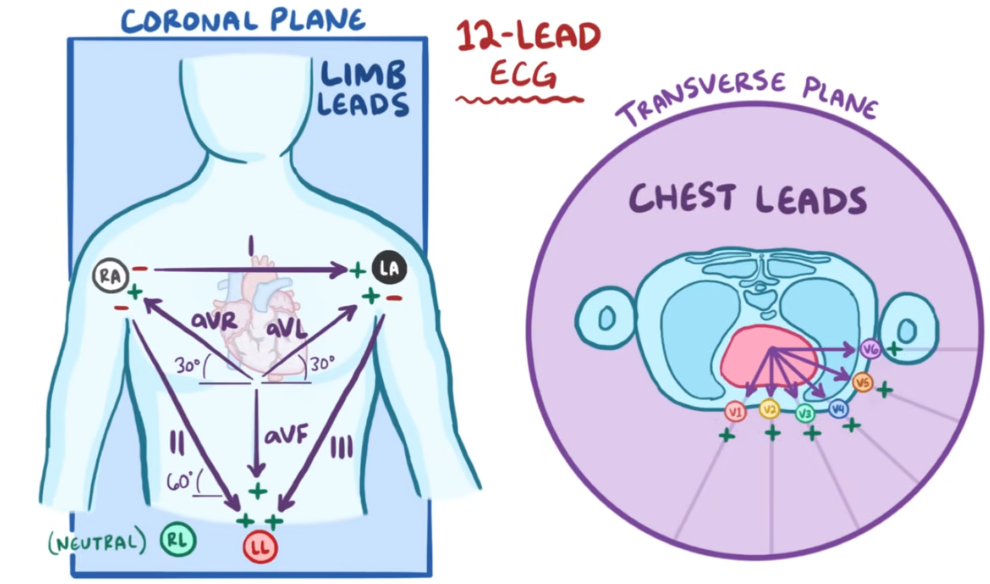
\includegraphics[width=0.7\linewidth]{images/pos-elettrodi.png}
    \caption{Posiziamento degli elettrodi}
    \label{fig:placeholder}
\end{figure}

\begin{itemize}
    \item \textbf{V1-V6}: sono i grafi generati dai sei elettrodi precordiali, numerati dal mediastino (V1) alla parte laterale del corpo (V6).  
    \item \textbf{aVR}: grafo proveniente dal braccio destro (polso o spalla).
    \item \textbf{aVL}: grafo proveniente dal braccio sinistro. (polso o spalla).
    \item \textbf{aVF}: grafo proveniente dal piede sinistro (caviglia o gamba).
    \item \textbf{I}: utilizza il braccio destro come polo negativo e il braccio sinistro come polo positivo.
    \item \textbf{II}: utilizza il braccio destro come polo negativo e il piede sinistro come polo positivo.
    \item \textbf{III}: utilizza il braccio sinistro come polo negativo e il piede sinistro come polo positivo.
\end{itemize}
L'elettrodo nel piede destro viene utilizzato dall'elettrocardiografo per minimizzare il rumore e ridurre le interferenze elettriche, come fosse la massa di un circuito elettrico.

\subsection{Calcolo delle Derivazioni}
Le dodici derivazioni dell'ECG non sono tutte ottenute allo stesso modo: si distinguono infatti le \textit{derivazioni bipolari}, teorizzate da Einthoven, le \textit{derivazioni unipolari aumentate}, teorizzate da Goldberger.

\subsubsection{Derivazioni pericordiali}
Le derivazioni \textit{V1-V6} utilizzano un punto di riferimento comune, a potenziale zero, chiamato \textit{terminale centrale di Wilson}: viene calcolato come la media dei tre elettrodi periferici, escludendo il piede destro.

\subsubsection{Derivazioni di Einthoven}
Le derivazioni \textit{I}, \textit{II} e \textit{III} costituiscono il cosiddetto \textbf{triangolo di Einthoven}: i tre elettrodi periferici (braccio destro, braccio sinistro e piede sinistro) vengono idealmente collegati tra loro a formare un triangolo equilatero, con il cuore posizionato al centro. Ogni derivazione misura la differenza di potenziale tra una coppia di elettrodi (da cui il termine \textit{bipolare}):
\begin{itemize}
    \item \textbf{I} = braccio sinistro (+) $-$ braccio destro ($-$)
    \item \textbf{II} = piede sinistro (+) $-$ braccio destro ($-$)
    \item \textbf{III} = piede sinistro (+) $-$ braccio sinistro ($-$)
\end{itemize}
Dalla geometria del triangolo discende la cosiddetta \textbf{legge di Einthoven}, secondo cui la somma algebrica delle derivazioni I e III è pari alla derivazione II:
\[
I + III = II
\]
Questa relazione è utile anche come controllo di coerenza del tracciato registrato.

\subsubsection{Derivazioni di Goldberger}
Le derivazioni \textit{aVR}, \textit{aVL} e \textit{aVF} sono invece \textit{unipolari}: misurano il potenziale di un singolo elettrodo periferico rispetto a un riferimento comune, chiamato \textit{terminale centrale}. Goldberger propose di costruire tale riferimento come media dei due elettrodi periferici diversi da quello esplorato, escludendo però quest'ultimo dal calcolo del riferimento stesso. Questo accorgimento fa sì che il segnale ottenuto risulti amplificato del 50\% rispetto a quanto si otterrebbe usando il \textit{terminale centrale di Wilson} (media di tutti e tre gli elettrodi periferici), da cui il prefisso "a" nel nome:
\begin{itemize}
    \item \textbf{aVR} (\textit{augmented Vector Right}): esplora il braccio destro.
    \item \textbf{aVL} (\textit{augmented Vector Left}): esplora il braccio sinistro.
    \item \textbf{aVF} (\textit{augmented Vector Foot}): esplora il piede sinistro.
\end{itemize}

Le sei derivazioni periferiche (I, II, III, aVR, aVL, aVF), pur derivando dagli stessi tre elettrodi fisici, osservano il cuore secondo angolazioni diverse sul piano frontale, distanziate tra loro di 30°: è proprio questa disposizione angolare a essere riorganizzata nel sistema Cabrera descritto più avanti.
\begin{figure}[h!]
    \centering
    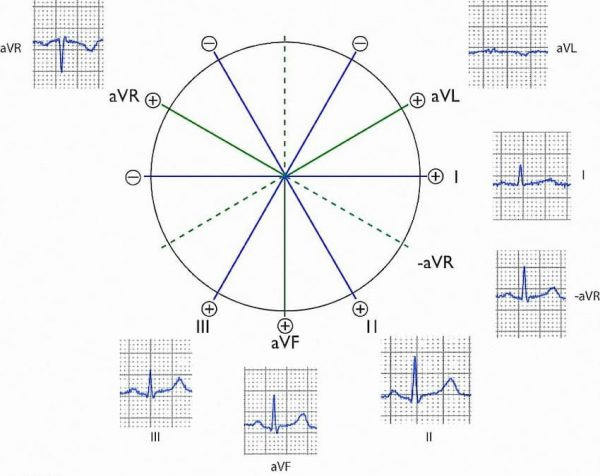
\includegraphics[width=0.7\linewidth]{images/visione_core.jpg}
    \caption{Viste prospettiche del cuore rispetto a Einthoven e Goldberger}
    \label{fig:vista_cuore}
\end{figure}

\subsection{Visibilità}

L'ECG a 12 derivazioni consente una buona visione del cuore offrendo una copertura complessiva di tutte le pareti cardiache. Le derivazioni inferiori (II, III, aVF) esplorano la parete inferiore, le derivazioni laterali (I, aVL, V5, V6) la parete laterale, mentre le derivazioni precordiali (V1--V4) forniscono informazioni sulla parete anteriore e sul setto interventricolare.

Ne consegue che alcune regioni risultano scarsamente rappresentate nella configurazione standard, come la parete posteriore e il ventricolo destro, che richiedono derivazioni aggiuntive per una valutazione completa.

Per questa ragione, le derivazioni di questa tipologia di ECG vengono tradizionalmente organizzate e interpretate in funzione della visione del ventricolo sinistro: ciascun gruppo di derivazioni corrisponde a una parete specifica di tale ventricolo, consentendo una lettura ordinata per regioni anatomiche. È proprio su questo principio che si fonda il sistema Cabrera, che propone una riorganizzazione delle derivazioni frontali secondo una sequenza anatomicamente continua relativamente all'angolo di osservazione del ventricolo, con l'obiettivo di rendere più intuitiva l'interpretazione dell'attività elettrica del ventricolo sinistro.

\begin{figure}[h!]
    \centering
    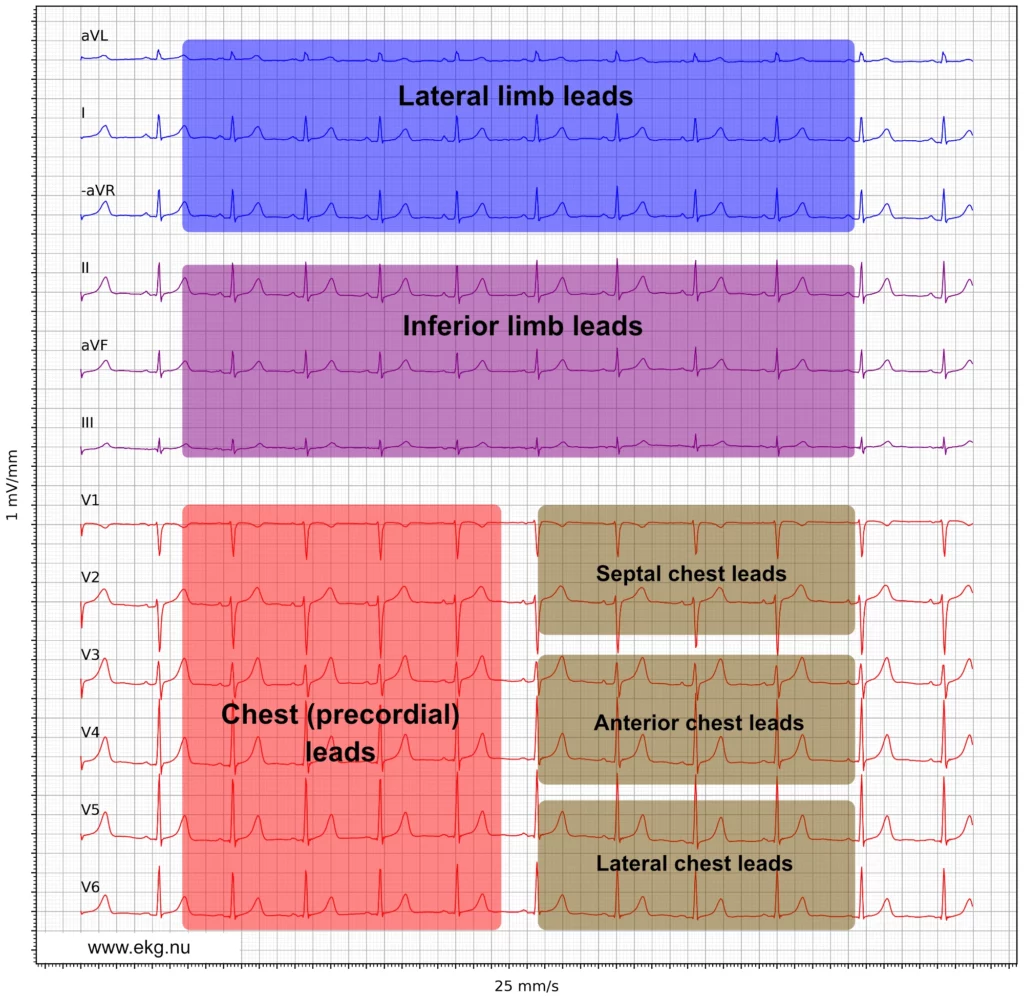
\includegraphics[width=0.50\linewidth]{images/12-lead-ecg-leads-limb-chest-cabrera.png}
    \caption{Sistema Cabrera}
    \label{fig:placeholder}
\end{figure}

\subsection{Lettura ECG}
L'elettrocardiografo presenta un diagramma per ogni derivazione. La differenza di potenziale, espressa in $mV$, è rappresentata sull'asse Y, mentre il tempo è rappresentato sull'asse delle X. L'ECG viene stampato su carta millimetrata caratterizzata da piccoli quadrati da un $mm$ di lato (riga fine) e grandi quadrati d $5\,mm$ di lato (riga spessa); in un elettrocardiografo ben calibrato e con velocità di stampa standard a $25\,mm/s$, avremo che $10\,mm$ (due blocchi grandi) sull'asse Y corrispondono ad $1\,mV$, e $10\,mm$ sull'asse delle X equivalgono a $400\,ms$.
 Le fasi della contrazione cardiaca si presentano nell'ECG tramite un pattern ricorrente di diverse onde: la prima, chiamata \textbf{onda P}, rappresenta la depolarizzazione atriale, l’evento elettrico che innesca e precede la contrazione meccanica (sistole) atriale, ed è solitamente visibile nella maggior parte delle derivazioni; poi abbiamo il \textbf{complesso QRS}, che rappresenta la depolarizzazione ventricolare, l’evento elettrico che precede e innesca la sistole ventricolare, ed è composto da tre deflessioni distinte: l'\textit{onda Q} (prima deflessione negativa) data dalla depolarizzazione del setto interventricolare, l'\textit{onda R} (deflessione positiva principale) data dalla depolarizzazione delle pareti "libere", essendo il ventricolo sinistro con massa muscolare maggiore, il suo vettore predomina, infine abbiamo l'\textit{onda S} (seconda deflessione negativa) data dalla depolarizzazione alla base dei ventricoli, cioè nella parte alta, vicino ai grandi vasi. Il complesso QRS è di maggiore ampiezza e durata rispetto all'onda P, a indicare la maggiore massa muscolare dei ventricoli. Segue il \textbf{segmento ST}, un breve tratto isoelettrico che avviene tra la fine della depolarizzazione ventricolare e l'inizio della ripolarizzazione; in condizioni fisiologiche si trova sulla linea di base. Infine, l'\textbf{onda T} rappresenta la ripolarizzazione ventricolare, ovvero il ritorno delle cellule miocardiche allo stato di riposo in preparazione al ciclo successivo; è normalmente positiva nelle derivazioni in cui il complesso QRS presenta una deflessione principale positiva.

Ovviamente, la visibilità e la direzione delle onde non saranno le stesse per tutte le derivazioni perché, come detto in precedenza, gli elettrodi misurano i campi elettrici direzionati verso di essi. Quindi ogni derivazione mostrerà diversi aspetti del ciclo cardiaco, ad esempio, in V1 l'onda R è minuscola e la S è profonda mentre in V5-V6 è l'opposto, l'onda R è alta e la S è quasi assente.

\begin{figure}[h!]
    \centering
    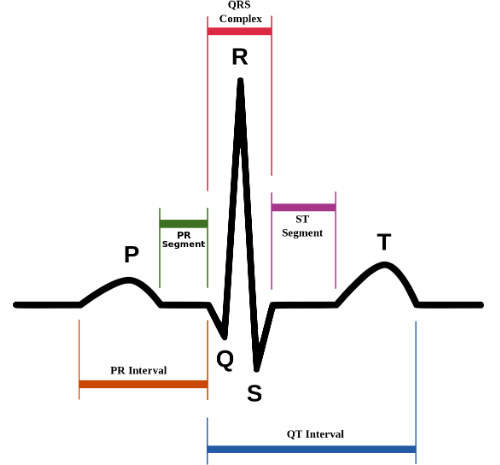
\includegraphics[width=0.4\linewidth]{images/onda-pqrst.jpg}
    \caption{onda P QRS T}
    \label{fig:placeholder}
\end{figure}

Tra le onde è possibile misurare alcuni \textbf{intervalli} di rilevanza clinica. L'\textbf{intervallo PR}, misurato dall'inizio dell'onda P all'inizio del complesso QRS, riflette il tempo di conduzione atrioventricolare, ovvero il ritardo fisiologico introdotto dal nodo atrioventricolare prima che l'impulso raggiunga i ventricoli; il suo valore normale è compreso tra $120$ e $200\,ms$. L'\textbf{intervallo QT}, misurato dall'inizio del complesso QRS alla fine dell'onda T, rappresenta la durata complessiva della sistole elettrica ventricolare, comprensiva sia della depolarizzazione che della ripolarizzazione; poiché dipende dalla frequenza cardiaca, viene spesso corretto con apposite formule (QTc) e il suo valore normale è generalmente inferiore a $440\,ms$ nell'uomo e $460\,ms$ nella donna.

\subsubsection{Ritmo sinusale normale}
Viene definito \textbf{ritmo sinusale normale} un ritmo cardiaco in cui ogni impulso ha origine regolarmente dal nodo senoatriale, si propaga attraverso il sistema di conduzione in modo fisiologico e produce sull'ECG un pattern caratteristico e ripetitivo. È importante precisare che la presenza di un ritmo sinusale normale indica esclusivamente la corretta origine e conduzione dell'impulso elettrico, non escludendo la presenza di patologie strutturali o funzionali del cuore.

I criteri che definiscono questo ritmo sono i seguenti:
\begin{itemize}
    \item Ogni complesso QRS deve essere preceduto da un'onda P
    \item L'intervallo PR deve essere costante e compreso tra $120$ e $200\,ms$
    \item La frequenza cardiaca deve essere compresa tra $60$ e $100$ battiti al minuto
    \item I complessi QRS devono essere regolarmente distanziati tra loro
    \item L'onda P deve essere positiva in $I$ e $II$, e negativa in $aVR$  
\end{itemize}

%---------------CAPITOLO 2---------------

%---------------CAPITOLO 3---------------
\chapter{Stato dell'arte}

Il rilevamento automatico del malposizionamento degli elettrodi è un problema studiato in letteratura da diversi decenni, molto prima della diffusione delle tecniche di deep learning. La maggior parte dei metodi storicamente proposti, e tuttora impiegati nella pratica clinica e nei software degli elettrocardiografi commerciali, si basa su \textbf{criteri morfologici e regole derivate dall'elettrofisiologia}, piuttosto che su modelli appresi da grandi quantità di dati. Solo recentemente, e quasi esclusivamente in ambito di ricerca, sono stati proposti approcci basati su machine learning e deep learning. Questo capitolo ripercorre entrambe le famiglie di metodi, evidenziandone vantaggi, limiti e il lavoro qui spiegato rispetto ad esse.

\section{Metodi classici basati su regole}

\subsection{Scambi degli elettrodi periferici}

Gli scambi che coinvolgono gli elettrodi periferici (braccio destro, braccio sinistro, gamba sinistra) sono la categoria di malposizionamento più studiata, poiché il loro effetto sulle derivazioni di Einthoven e di Goldberger è descrivibile in modo esatto tramite le equazioni geometriche presentate nel Capitolo 2 \ref{pos_elettrodi}. I metodi classici sfruttano proprio questa prevedibilità, costruendo alberi decisionali basati sulla polarità e sull'ampiezza dell'onda P, sulla morfologia del complesso QRS e sulla relazione tra le derivazioni~\cite{paul2023lead}.

Un criterio storicamente molto utilizzato è quello della \textbf{polarità dell'onda P in derivazione aVR}: in condizioni di corretto posizionamento e ritmo sinusale, l'onda P è normalmente negativa in aVR; la maggior parte degli scambi tra gli elettrodi periferici che non coinvolgono l'elettrodo di terra produce invece un'onda P positiva in questa derivazione, un segnale facilmente verificabile in modo automatico~\cite{paul2023lead}. In modo analogo, lo scambio tra braccio sinistro e gamba sinistra, che non altera la polarità in aVR, può essere identificato confrontando l'ampiezza dell'onda P nelle derivazioni I e II: un'ampiezza maggiore in I rispetto a II è indicativa di questo specifico scambio~\cite{paul2023lead}.

Un secondo filone di lavori sfrutta la \textbf{direzione di inscrizione del vettore P nel piano frontale}: in condizioni fisiologiche il ciclo descritto dal vettore P durante la depolarizzazione atriale segue, con rarissime eccezioni, un verso antiorario; un'inversione di questo verso, unita alla posizione osservata dell'asse dell'onda P, permette di classificare con buona accuratezza (secondo alcuni studi fino a oltre il 90\% dei casi) quale coppia di elettrodi periferici sia stata scambiata, anche senza disporre di un tracciato di riferimento del medesimo paziente~\cite{ho2001pwave}.

Un terzo approccio, complementare ai precedenti, si basa sulla \textbf{ridondanza informativa} intrinseca delle sei derivazioni periferiche, che sono tutte calcolabili a partire dai medesimi tre potenziali misurati agli elettrodi. Alcuni algoritmi ricostruiscono le derivazioni attese a partire da un sottoinsieme di esse e le confrontano, tramite indici di correlazione, con quelle effettivamente registrate; una discrepanza sistematica tra derivazioni ricostruite e osservate è indicativa di uno scambio~\cite{kors2000correlation, kors2001accurate}. Un esempio di questo filone è l'analisi delle correlazioni incrociate tra le derivazioni periferiche e la derivazione V6, che si è dimostrata efficace anche in assenza di annotazioni di riferimento~\cite{jekova2016interlead}.

\subsection{Scambi degli elettrodi precordiali}

Il rilevamento degli scambi tra elettrodi precordiali (V1--V6) è generalmente considerato più complesso rispetto a quello degli elettrodi periferici, poiché non esiste per queste derivazioni un vincolo algebrico altrettanto rigido quanto la legge di Einthoven: l'informazione discriminante è quindi prevalentemente morfologica. I metodi classici sfruttano principalmente la \textbf{progressione dell'onda R} attraverso le derivazioni V1--V6, che in condizioni normali cresce in modo pressoché monotono da V1 a V5--V6, mentre l'onda S segue l'andamento opposto. Un'interruzione o un'inversione di questa progressione tra derivazioni adiacenti è un indicatore classico, sebbene non sempre specifico, di un possibile scambio o di un posizionamento verticale non corretto (ad esempio in uno spazio intercostale errato)~\cite{jekova2016interlead}.

In modo analogo a quanto visto per le derivazioni periferiche, anche per i precordiali sono stati proposti metodi basati sulla \textbf{correlazione tra derivazioni adiacenti}: la somiglianza morfologica attesa tra V1 e V2, o più in generale tra derivazioni vicine sul torace, tende ad aumentare in modo anomalo quando due elettrodi vengono scambiati tra loro, un effetto quantificabile con semplici coefficienti di similitudine~\cite{jekova2015precordial, jekova2016interlead}.

\subsection{Limiti dei metodi classici}

I metodi basati su regole presentano il vantaggio di essere interpretabili, computazionalmente leggeri e, in molti casi, già integrati nel software degli elettrocardiografi commerciali. Tuttavia, essi condividono alcuni limiti strutturali: le soglie e le regole utilizzate sono spesso calibrate su popolazioni o dataset specifici e generalizzano male in presenza di ritmi non sinusali, di alterazioni patologiche della morfologia dell'onda P o del complesso QRS, o di rumore significativo sul tracciato~\cite{batchvarov2007incorrect}; inoltre, la loro accuratezza varia molto a seconda della specifica coppia di elettrodi scambiati, risultando generalmente più bassa per gli scambi precordiali e per gli scambi periferici che coinvolgono l'elettrodo di terra, per i quali l'effetto sul tracciato è meno marcato~\cite{kors2001accurate, batchvarov2007incorrect}. Già a metà degli anni '90 questi limiti avevano motivato i primi tentativi di sostituire, almeno in parte, le regole scritte a mano con modelli appresi dai dati, ad esempio tramite reti neurali artificiali applicate al riconoscimento degli scambi periferici~\cite{heden1995ann}.

\section{Approcci basati su apprendimento automatico e deep learning}

Negli ultimi anni, un numero sempre più grande di lavori ha affrontato il problema del rilevamento del malposizionamento con un approccio mirato alla classificazione supervisionata, affidandosi a tecniche di apprendimento automatico piuttosto che a regole scritte manualmente. È importante sottolineare che, ad oggi, questi approcci restano in larga parte confinati alla ricerca accademica~\cite{rjoob2020review}: nella pratica clinica corrente il controllo del corretto posizionamento degli elettrodi si basa quasi esclusivamente sui criteri a regole descritti nella sezione precedente, o sulla verifica visiva da parte del personale sanitario.

Un primo filone di lavori utilizza algoritmi di \textbf{machine learning tradizionale} (support vector machine, alberi decisionali, k-nearest neighbor) applicati a feature estratte manualmente dal tracciato, quali ampiezze e durate delle onde, indici di correlazione tra derivazioni e parametri morfologici del complesso QRS~\cite{han2014svm}. Studi di questo tipo, focalizzati in particolare sul rilevamento dello scambio delle derivazioni precordiali V1 e V2, riportano accuratezze nell'ordine dell'85--95\% a seconda dello spazio intercostale coinvolto e dell'algoritmo di selezione delle feature utilizzato.~\cite{rjoob2019datadriven}.

Un secondo filone, più recente, applica tecniche di \textbf{deep learning} direttamente al segnale grezzo, senza una fase esplicita di estrazione manuale delle feature. Le architetture proposte in letteratura sono in prevalenza reti convoluzionali monodimensionali (CNN 1D), talvolta alleggerite per essere eseguibili su dispositivi con risorse computazionali limitate~\cite{huang2024lightweight}, addestrate a distinguere il tracciato correttamente posizionato da diverse tipologie di scambio simulato, sia sulle derivazioni periferiche sia su quelle precordiali~\cite{rjoob2021jmir, huang2024lightweight, alves2025telecardiology}. Questi lavori riportano, in generale, prestazioni superiori rispetto ai corrispondenti metodi basati su feature manuali, a fronte però di una minore interpretabilità del modello e di una forte dipendenza dalla qualità e dalla rappresentatività del dataset di addestramento~\cite{alves2025telecardiology}, un aspetto particolarmente rilevante dato che, come nel presente lavoro, tali dataset sono quasi sempre costruiti simulando artificialmente gli scambi a partire da tracciati correttamente acquisiti.

Un aspetto comune alla gran parte dei lavori esistenti, sia classici sia basati su deep learning, è che le diverse derivazioni vengono tipicamente trattate come segnali indipendenti, o al più confrontate a coppie tramite indici di correlazione, senza modellare esplicitamente la struttura spaziale complessiva del sistema delle dodici derivazioni. Ad oggi, l'impiego di architetture a grafo per rappresentare esplicitamente la geometria spaziale delle derivazioni ECG in questo specifico compito non risulta ampiamente esplorato in letteratura; è proprio in questo spazio che si colloca il contributo originale proposto nel Capitolo 6 di questa tesi, dove la relazione spaziale tra derivazioni viene resa esplicita al modello tramite una matrice di adiacenza costruita sulla geometria reale del sistema di acquisizione, anziché essere lasciata implicita o appresa indirettamente dai dati; viengono oltretutto esplorate un'architettura CNN monodimensionale e un MLP, in modo da poter esplorere tutte le strade plausibili nel campo del deep learning.

\section{Posizionamento del presente lavoro}

Alla luce di quanto discusso, il presente lavoro si colloca all'intersezione tra i due filoni descritti: da un lato adotta un'architettura di deep learning, coerentemente con la tendenza più recente della letteratura; dall'altro cerca di superare il limite comune alla maggior parte dei modelli esistenti, ovvero il trattamento sostanzialmente indipendente delle singole derivazioni, incorporando esplicitamente nell'architettura l'informazione geometrica relativa alla disposizione spaziale degli elettrodi. I dettagli della pipeline di simulazione degli scambi e dell'architettura proposta sono presentati rispettivamente nei Capitoli \ref{chap_5} e \ref{chap_6}.
%---------------CAPITOLO 3---------------

%---------------CAPITOLO 4---------------
\chapter{Basi matematiche ed elaborazione del segnale}

\section{Fondamenta matematiche}

Prima di affrontare le tecniche di elaborazione del segnale ECG è necessario introdurre gli strumenti matematici su cui esse si fondano. Questa sezione presenta le trasformate fondamentali per l'analisi dei segnali, la teoria dei filtri lineari e il concetto di funzione di trasferimento, che costituiranno il riferimento teorico per tutte le sezioni successive~\cite{oppenheim1996signals, oppenheim1997dsp}.

\subsection{Fondamenti matematici per l'analisi dei segnali}

\subsubsection{Il segnale ECG come oggetto matematico}
Il segnale ECG nel mondo fisico è un segnale \textbf{continuo nel tempo}, formalmente una funzione:
\[
x : \mathbb{R} \to \mathbb{R}, \quad t \mapsto x(t)
\]
dove $t$ è il tempo in secondi e $x(t)$ è la differenza di potenziale in millivolt misurata tra due elettrodi. Presenta una struttura morfologica ripetitiva, corrispondente al ciclo PQRST ma non è strettamente periodico, poiché la durata di ogni ciclo varia leggermente nel tempo. Tale variabilità, nota come \textit{Heart Rate Variability} (HRV), costituisce una fonte di informazione clinicamente rilevante e sarà trattata nella sezione dedicata all'analisi nel dominio del tempo.

la funzione $x(t)$ appartiene allo spazio $L^2(\mathbb{R})$, ovvero è una funzione a \textbf{energia finita}:
\[
E = \int_{-\infty}^{+\infty} |x(t)|^2 \, dt < \infty
\]
Questa proprietà è fondamentale: garantisce l'esistenza della trasformata di Fourier e la validità di tutte le operazioni di filtraggio che verranno trattate nelle sezioni successive.

\subsubsection{Trasformata di Laplace}
\label{trasform_laplace}
La trasformata di Laplace è lo strumento fondamentale per l'analisi dei sistemi lineari \textbf{a tempo continuo}~\cite{oppenheim1996signals}. Data una funzione $x(t) : \mathbb{R} \to \mathbb{R}$ causale (ovvero nulla per $t < 0$), la sua trasformata di Laplace unilaterale è definita come:
\[
X(s) = \mathcal{L}\{x(t)\} = \int_{0}^{+\infty} x(t)\, e^{-st}
\, dt
\]
dove $s = \sigma + j\omega \in \mathbb{C}$ è la variabile complessa, con $\sigma \in \mathbb{R}$ parte reale e $\omega \in \mathbb{R}$ parte immaginaria. L'integrale converge nella \textbf{regione di convergenza} (ROC), ovvero l'insieme dei valori di $s$ per cui l'integrale esiste finito.

La trasformata inversa di Laplace è data dall'integrale di Bromwich:
\[
x(t) = \mathcal{L}^{-1}\{X(s)\} = \frac{1}{2\pi j}
\int_{\sigma - j\infty}^{\sigma + j\infty} X(s)\, e^{st} \, ds
\]
In pratica, l'antitrasformata viene quasi sempre calcolata tramite scomposizione in frazioni parziali e utilizzo di tavole delle trasformate note, evitando il calcolo diretto dell'integrale.

\paragraph{Proprietà fondamentali.}
Le proprietà della trasformata di Laplace che risultano più utili nell'analisi dei sistemi sono le seguenti. La \textbf{linearità} garantisce che:
\[
\mathcal{L}\{\alpha\, x(t) + \beta\, y(t)\} =
\alpha\, X(s) + \beta\, Y(s)
\]
La proprietà di \textbf{derivazione} trasforma la derivata nel dominio del tempo in una moltiplicazione nel dominio di $s$:
\[
\mathcal{L}\left\{\frac{d^n x}{dt^n}\right\} = s^n X(s) -
\sum_{k=0}^{n-1} s^{n-1-k}\, x^{(k)}(0^-)
\]
che per condizioni iniziali nulle si riduce a $s^n X(s)$. Questa proprietà è alla base della descrizione dei sistemi dinamici: un'equazione differenziale nel dominio del tempo diventa un'equazione algebrica nel dominio di $s$, molto più semplice da trattare.

La proprietà di \textbf{convoluzione} stabilisce che:
\[
\mathcal{L}\{x(t) * h(t)\} = X(s) \cdot H(s)
\]
dove $*$ indica la convoluzione. L'uscita di un sistema lineare è la convoluzione dell'ingresso con la risposta impulsiva del sistema; nel dominio di $s$ tale operazione diventa una semplice moltiplicazione, rendendo molto più agevole l'analisi dei sistemi in cascata.

\paragraph{Relazione con la trasformata di Fourier.}
La trasformata di Fourier si ottiene dalla trasformata di Laplace valutandola solamente sull'asse immaginario, ovvero ponendo $\sigma = 0$ e $s = j\omega = j 2\pi f$:

\[
X(j\omega) = X(s)\big|_{s = j\omega} =
\int_{-\infty}^{+\infty} x(t)\, e^{-j\omega t} \, dt
\]
Questa relazione è valida se e solo se il segnale sia strettamente \textit{causale} (come definito in \ref{trasform_laplace}) e l'asse immaginario appartenga alla ROC.

Geometricamente, la trasformata di Fourier è la restrizione della trasformata di Laplace alla retta verticale $\text{Re}(s) = 0$ nel piano complesso. Mentre la trasformata di Laplace descrive il comportamento transitorio e la stabilità di un sistema, la trasformata di Fourier ne descrive la risposta in regime sinusoidale stazionario, ovvero la risposta in frequenza.

\subsubsection{Trasformata di Fourier}
La trasformata di Fourier estende il concetto di serie di Fourier (valido per segnali periodici) ai segnali aperiodici a \emph{energia finita}~\cite{oppenheim1996signals}. Data $x(t) \in L^2(\mathbb{R})$, la trasformata di Fourier è definita come:
\[
X(f) = \mathcal{F}\{x(t)\} =
\int_{-\infty}^{+\infty} x(t)\, e^{-j2\pi f t} \, dt
\]
e la trasformata inversa come:
\[
x(t) = \mathcal{F}^{-1}\{X(f)\} =
\int_{-\infty}^{+\infty} X(f)\, e^{j2\pi f t} \, df
\]
$X(f)$ è in generale una funzione a valori complessi. Il suo modulo $|X(f)|$ è detto \textbf{spettro di ampiezza} e descrive l'intensità di ciascuna componente frequenziale, mentre la sua fase $\Delta X(f)$ indica lo sfasamento di ogni componente sinusoidale. La quantità $|X(f)|^2$ è detta \textbf{densità spettrale di energia} e il teorema di Parseval garantisce la conservazione dell'energia nelledue rappresentazioni:
\[
\int_{-\infty}^{+\infty} |x(t)|^2\, dt =
\int_{-\infty}^{+\infty} |X(f)|^2\, df
\]
Una proprietà fondamentale è quella di derivazione nel dominio del tempo: sia $f(t)$ continua e derivabile, siano $f(t)$ e $f^{'}(t)$ integrabili a energia finita, allora possiamo dire che derivare una funzione nel tempo (dominio reale) equivale a moltiplicare la sua trasformata di Fourier per $j\omega$
\[
\mathcal{F}\{f^{'}(t)\}=j\omega\mathcal{F}\{f(t)\} 
\]

\paragraph{Trasformata di Fourier discreta (DFT).}
Per segnali disponibili come \textbf{sequenze finite} di $N$ campioni $\{x[n]\}_{n=0}^{N-1}$, la Trasformata di Fourier Discreta è definita come~\cite{oppenheim1997dsp}:
\[
X[k] = \sum_{n=0}^{N-1} x[n]\, e^{-j2\pi kn/N},
\quad k = 0, 1, \ldots, N-1
\]
dove $k$ indicizza le frequenze discrete $f_k = k \cdot f_s / N$. La trasformata inversa è:
\[
x[n] = \frac{1}{N} \sum_{k=0}^{N-1} X[k]\, e^{j2\pi kn/N},
\quad n = 0, 1, \ldots, N-1
\]
Il calcolo diretto della DFT richiede $\mathcal{O}(N^2)$ operazioni. L'\textbf{algoritmo FFT} (\textit{Fast Fourier Transform}) riduce questa complessità a $\mathcal{O}(N \log N)$ sfruttando la simmetria della DFT, rendendo l'analisi spettrale computazionalmente praticabile anche su segnali di lunga durata.

\subsubsection{Trasformata Z}
La trasformata Z è l'analogo discreto della trasformata di Laplace e costituisce lo strumento naturale per l'analisi e la progettazione di filtri digitali~\cite{oppenheim1997dsp}. Data una sequenza discreta $x[n]$, la sua trasformata Z bilaterale è definita come:
\[
X(z) = \mathcal{Z}\{x[n]\} = \sum_{n=-\infty}^{+\infty}
x[n]\, z^{-n}, \quad z \in \mathbb{C}
\]
La serie converge in un sottoinsieme del piano complesso detto \textbf{regione di convergenza} (ROC). Il termine $z^{-n}$ ha un'interpretazione geometrica diretta: per $z = r e^{j\omega}$, la trasformata Z valuta la sequenza $x[n]$ pesata da un'esponenziale complessa a frequenza $\omega$ e ampiezza $r^{-n}$.

\paragraph{Significato di $z^{-1}$.}
L'elemento fondamentale della trasformata Z è la proprietà di ritardo: moltiplicare per $z^{-k}$ nel dominio Z corrisponde a ritardare la sequenza di $k$ campioni nel dominio del tempo:
\[
\mathcal{Z}\{x[n-k]\} = z^{-k}\, X(z)
\]
Questa proprietà rende $z^{-1}$ interpretabile come un \textbf{operatore di ritardo unitario}: un elemento che restituisce il campione precedente. È l'elemento fondamentale con cui si costruiscono i filtri digitali, poiché qualsiasi equazione alle differenze con campioni ritardati si traduce immediatamente in un'espressione algebrica in $z$.

\paragraph{Relazione con la trasformata di Fourier a tempo discreto (DTFT).}
Valutando la trasformata Z sulla circonferenza unitaria $|z| = 1$, ovvero ponendo $z = e^{j\omega}$, si ottiene la trasformata di Fourier a tempo discreto (DTFT):
\[
X\!\left(e^{j\omega}\right) = X(z)\big|_{z=e^{j\omega}}
= \sum_{n=-\infty}^{+\infty} x[n]\, e^{-j\omega n}
\]
La DTFT è una funzione \textit{continua} della variabile di frequenza $\omega$ (o, equivalentemente, di $f = \omega f_s / 2\pi$), definita per sequenze $x[n]$ generalmente di lunghezza infinita. Essa generalizza al caso discreto la trasformata di Fourier continua, ed esiste (in senso classico) solo per le sequenze la cui ROC della trasformata Z include la circonferenza unitaria.

\paragraph{Dalla DTFT alla DFT.}
La \textbf{DFT}, definita in precedenza per sequenze finite di $N$ campioni, si ottiene \textbf{campionando la DTFT} in $N$ punti equispaziati lungo la circonferenza unitaria, alle frequenze discrete:
\[
\omega_k = \frac{2\pi k}{N}, \qquad k = 0, 1, \ldots, N-1
\]
ovvero:
\[
X[k] = X\!\left(e^{j\omega}\right)\Big|_{\omega = \frac{2\pi k}{N}}
= X\!\left(e^{j2\pi k/N}\right)
\]
La DFT è dunque una sequenza \textbf{discreta} di $N$ valori, mentre la DTFT è una funzione continua di $\omega$, di cui la DFT ne rappresenta un campionamento in frequenza.

\paragraph{Proprietà fondamentali.}
Le proprietà più rilevanti per l'analisi dei filtri digitali sono la \textbf{linearità}:
\[
\mathcal{Z}\{\alpha\, x[n] + \beta\, y[n]\} =
\alpha\, X(z) + \beta\, Y(z)
\]
e la proprietà di \textbf{convoluzione}, analoga a quella della trasformata di Laplace:
\[
\mathcal{Z}\{x[n] * h[n]\} = X(z) \cdot H(z)
\]
dove $*$ indica la convoluzione discreta. Come nel caso continuo, questa proprietà trasforma l'operazione di filtraggio, che nel dominio del tempo è una convoluzione, in una moltiplicazione nel dominio Z.

\subsection{Spline}

La spline viene utilizzata per problemi di interpolazione e nasce per sopperire all'utilizzo di un singolo polinomio che in presenza di molti punti diventa di grado molto alto, generando delle brusche oscillazioni nella funzione interpolante, definito come fenomeno di Runge.

Una spline di grado $n$ su una partizione $\{t_1,\dots,t_k\}$ è una funzione $S(t)$ tale che:
\begin{itemize}
	\item su ogni intervallo $[t_i,t_{i+1}]$ ci sia un polinomio di grado $\le n$
	\item è continua insieme alle derivate fino al grado $n-1$ nei punti di raccordo $t_i$
\end{itemize}
La regolarità $C^{n-1}$ nei punti di raccordo descritta sopra rappresenta la condizione di \emph{massima regolarità teorica} raggiungibile per una spline di grado $n$, e vale esclusivamente nel caso di \emph{nodi semplici}, cioè quando ogni nodo $t_i$ compare una sola volta nella partizione. Nel seguito, la trattazione si limiterà a questo caso. In presenza di \emph{nodi multipli} (un nodo ripetuto con molteplicità $m$), la regolarità nel punto di giunzione si riduce, cioè la spline risulta continua solamente fino alla derivata di ordine $n-m$, permettendo così di introdurre in modo controllato discontinuità o spigoli nella curva o nelle sue derivate.

\subsubsection{B-spline}

Le B-spline sono molto importanti, in quanto qualsiasi funzione spline può essere scritta come combinazione lineare di B-spline~\cite{unser1999splines}. Una proprietà fondamentale di esse è il \textbf{supporto compatto minimo}: data una B-spline di grado $n$, allora essa sarà non nulla solamente nell'intervallo determinato da $n+2$ nodi consecutivi; al di fuori di questo intervallo la funzione assume valore zero.

Questa funzione presenta diversi vantaggi: il primo è dato dal fatto che, grazie al supporto compatto minimo, spostando un nodo, o modificando un coefficiente, la modifica si propaga solamente a un numero \emph{limitato e ben definito} di intervalli adiacenti, cioè quelli coperti dal supporto della B-spline di grado $n$, ovvero $n+2$ nodi consecutivi, mentre il resto della curva, al di fuori di questa finestra, rimane invariato; il secondo nasce di conseguenza. Infatti, la B-spline risulta molto efficiente in quanto il calcolo di un punto della curva non richiede l'elaborazione di tutta la curva considerando tutti i punti, ma solamente delle B-spline il cui supporto contiene quel punto. Infine sono particolarmente indicate per i filtri FIR~\cite{unser1999splines}.

\paragraph{Definizione} La B-spline di grado $0$ è una semplice funzione rettangolare:
\[
\beta^0(t)= \begin{cases}
	1 & 0\le t\le 1 \\
	0 & altrimenti
\end{cases}
\]
Le B-spline di grado $n$ sono continue insieme alle loro derivate fino all'ordine $n-1$, le B-spline di ordine superiore si costruiscono per \textbf{auto-convoluzione}~\cite{unser1999splines}:
\[
\beta^n(t)=\underbrace{\beta^0*\beta^0\dots*\beta^0}_\text{n+1 volte}
\]

\paragraph{Metodi per il calcolo della convoluzione.} Esistono due modi principali per calcolare un operazione di convoluzione:
\begin{description}
	\item[Integrale di convoluzione]
	In generale l'operazione di convoluzione tra due funzioni $f(t)$ e $g(t)$ è:
	\[
	(f*g)(t)=\int^{+\infty}_{-\infty}{f(\alpha)g(t-\alpha)\,d\alpha} 
	\]
	In questo caso $f$ e $g$ sono la stessa funzione. In termini grafici, questa operazione equivale a prendere la funzione rettangolare $\beta^0$ e scorrerla come una finestra sull'altra; è per questo motivo che $\beta^1$ è una funzione triangolare.
	
	\item[Trasformata di Fourier]
	Per la proprietà di convoluzione delle trasformate, una qualsiasi operazione di convoluzione nel dominio reale diventa una semplice moltiplicazione nel dominio delle trasformate:
	\[
	\mathcal{F}\{f*g\}(\omega)=\mathcal{F}\{f\}(\omega)\cdot\mathcal{F}\{g\}(\omega) 
	\]
	Ora calcoliamo la trasformata di $\beta^0$:
	\[
	\hat{\beta}^0(\omega)=\int^{+\infty}_{-\infty}{\beta}^0(t)\cdot e^{-j\omega t}\,dt=\int^{1}_{0}{e^{-j\omega t}\,dt}=\left[\frac{e^{-j\omega t}}{-j\omega}\right]^1_0=\frac{1-e^{-j\omega}}{j\omega}
	\]
	Quindi ci basterà elevare il risulato finale alla $n+1$ per ottenere una B-spline di grado $n$:
	\[
	\hat{\beta}^n=\left(\frac{1-e^{-j\omega}}{j\omega}\right)^{n+1}
	\]
\end{description}

\subsection{Filtri lineari e funzione di trasferimento}

Un \textbf{filtro digitale} è un sistema che trasforma una sequenza di ingresso $x[n]$ in una sequenza di uscita $y[n]$ secondo una relazione definita da un'equazione alle differenze. Un sistema si dice \textbf{lineare} se rispetta il principio di sovrapposizione: la risposta alla somma di due ingressi è uguale alla somma delle risposte ai singoli ingressi, ovvero per qualsiasi scalari $\alpha, \beta$ e ingressi $x_1[n], x_2[n]$~\cite{oppenheim1997dsp}:
\[
T\{\alpha\, x_1[n] + \beta\, x_2[n]\} =
\alpha\, T\{x_1[n]\} + \beta\, T\{x_2[n]\}
\]
Un sistema si dice \textbf{tempo-invariante} se la sua risposta non dipende dall'istante temporale assoluto in cui viene applicato l'ingresso: ritardare l'ingresso di $k$ campioni produce semplicemente un'uscita ritardata di $k$ campioni, senza alterarne la forma. Un sistema che gode di entrambe le proprietà è detto \textbf{LTI} (\textit{Linear Time-Invariant}) e costituisce la classe di sistemi più ampiamente studiata nell'elaborazione dei segnali, poiché è completamente caratterizzata dalla propria \textbf{risposta impulsiva} $h[n]$, ovvero dall'uscita prodotta quando l'ingresso è un impulso unitario $\delta[n]$.

\paragraph{Equazione alle differenze.}
La forma generale di un filtro LTI causale è:
\[
\sum_{k=0}^{N} a_k\, y[n-k] = \sum_{m=0}^{M} b_m\, x[n-m]
\]
con $a_0 = 1$ per convenzione. I coefficienti $\{b_m\}$ pesano i campioni correnti e passati dell'ingresso (parte \textit{feedforward}), mentre i coefficienti $\{a_k\}$ con $k \geq 1$ pesano i campioni passati dell'uscita (parte \textit{feedback}). La presenza o assenza di quest'ultima determina la distinzione tra le due grandi famiglie di filtri digitali.

\paragraph{Funzione di trasferimento.}
Applicando la trasformata Z all'equazione alle differenze e sfruttando la proprietà di ritardo $\mathcal{Z}\{y[n-k]\} = z^{-k} Y(z)$, si ottiene:
\[
Y(z) \sum_{k=0}^{N} a_k\, z^{-k} =
X(z) \sum_{m=0}^{M} b_m\, z^{-m}
\]
La \textbf{funzione di trasferimento} è il rapporto tra la trasformata Z dell'uscita e quella dell'ingresso a condizioni iniziali nulle:
\[
H(z) = \frac{Y(z)}{X(z)} =
\frac{\displaystyle\sum_{m=0}^{M} b_m\, z^{-m}}
{\displaystyle\sum_{k=0}^{N} a_k\, z^{-k}}
\]
$H(z)$ è una funzione razionale in $z^{-1}$ che contiene tutta l'informazione sul comportamento del filtro. I valori di $z$ per cui il numeratore si annulla sono detti \textbf{zeri}; i valori per cui il denominatore si annulla sono detti \textbf{poli}. La posizione di poli e zeri nel piano complesso determina completamente le proprietà del filtro.

\paragraph{Risposta in frequenza.}
Valutando $H(z)$ sulla circonferenza unitaria si ottiene la \textbf{risposta in frequenza} del filtro:
\[
H\!\left(e^{j2\pi f/f_s}\right) = |H(f)|\, e^{j\Delta H(f)}
\]
Il modulo $|H(f)|$ è detto \textbf{risposta in ampiezza} e descrive quanto il filtro amplifica o attenua ciascuna componente frequenziale; la fase $\Delta H(f)$ descrive il ritardo di fase introdotto. Un filtro ideale passa-basso con frequenza di taglio $f_c$ avrebbe:
\[
|H(f)| = \begin{cases} 1 & |f| \leq f_c \\ 0 & |f| > f_c
\end{cases}
\]
I filtri reali approssimano questo comportamento ideale con transizioni graduali tra banda passante e banda attenuata.

\subsubsection{Impulso unitario e risposta impulsiva.}
L'impulso unitario discreto, detto anche \textbf{delta di Kronecker}, è la sequenza definita come:
\[
\delta[n] = \begin{cases} 1 & n = 0 \\ 0 & n \neq 0 \end{cases}
\]
Esso costituisce l'elemento identità rispetto alla convoluzione discreta e gode di una proprietà fondamentale, detta \textbf{proprietà di campionamento}:
\[
\sum_{k=-\infty}^{+\infty} x[k]\, \delta[n - k] = x[n]
\]
che esprime il fatto che qualsiasi sequenza $x[n]$ può essere decomposta in una somma di impulsi traslati e pesati dai propri valori. Questa decomposizione, combinata con le proprietà di linearità e tempo-invarianza, implica che l'uscita di un sistema LTI a un ingresso arbitrario $x[n]$ è completamente determinata dalla risposta del sistema al solo impulso $\delta[n]$.

Si definisce \textbf{risposta impulsiva} $h[n]$ l'uscita di un sistema LTI quando l'ingresso è l'impulso unitario:
\[
h[n] = T\{\delta[n]\}
\]
dove $T\{\cdot\}$ indica l'operatore che descrive il sistema. La conoscenza di $h[n]$ è sufficiente a determinare l'uscita del sistema per qualsiasi ingresso $x[n]$, poiché per le proprietà LTI si ha:
\[
y[n] = \sum_{k=-\infty}^{+\infty} x[k]\, h[n-k] = x[n] * h[n]
\]
ovvero l'uscita è la \textbf{convoluzione discreta} dell'ingresso con la risposta impulsiva. Questo risultato, noto come \textbf{integrale di convoluzione discreto}, è il teorema centrale della teoria dei sistemi LTI: qualunque sistema lineare tempo-invariante è completamente caratterizzato dalla propria risposta impulsiva.

La funzione di trasferimento $H(z)$, introdotta nella sezione precedente come rapporto $Y(z)/X(z)$, coincide con la trasformata Z della risposta impulsiva:
\[
H(z) = \frac{Y(z)}{X(z)} = \mathcal{Z}\{h[n]\}
\]
Le due espressioni non sono definizioni indipendenti: la seconda segue direttamente dalla prima applicando la proprietà di convoluzione della trasformata Z all'identità $y[n] = x[n] * h[n]$.

La durata di $h[n]$ distingue le due grandi famiglie di filtri digitali. Se $h[n]$ è nulla al di fuori di un intervallo finito $[0, M]$, il filtro è detto FIR (\textit{Finite Impulse Response}); se $h[n]$ è non nulla per infiniti valori di $n$, tipicamente decade asintoticamente a zero, il filtro è detto IIR (\textit{Infinite Impulse Response}). Nel secondo caso la presenza di una componente di feedback nell'equazione alle differenze è la causa diretta della durata infinita della risposta impulsiva.

\subsubsection{Filtri FIR e IIR.}
Se tutti i coefficienti $a_k = 0$ per $k \geq 1$, allora il denominatore di $H(z)$ è costante e il filtro non ha poli (eccetto nell'origine). In questo caso l'uscita dipende solo dai campioni correnti e passati dell'ingresso, la risposta impulsiva ha durata finita e il filtro è detto \textbf{FIR} (\textit{Finite Impulse Response}):
\[
H_{FIR}(z) = \sum_{m=0}^{M} b_m\, z^{-m}
\]
I filtri FIR sono sempre stabili e possono essere progettati per avere \textbf{fase lineare}, proprietà che garantisce un ritardo costante e uguale per tutte le frequenze; condizione importante nell'analisi ECG per non distorcere la morfologia delle onde.

Se invece almeno un coefficiente $a_k \neq 0$, il filtro presenta un anello di retroazione: l'uscita attuale dipende anche dalle uscite passate. La risposta impulsiva ha durata infinita e il filtro è detto \textbf{IIR} (\textit{Infinite Impulse Response}):
\[
H_{IIR}(z) = \frac{\displaystyle\sum_{m=0}^{M} b_m\, z^{-m}}
{\displaystyle\sum_{k=0}^{N} a_k\, z^{-k}}
\]
I filtri IIR richiedono un numero di coefficienti inferiore rispetto ai FIR per ottenere la stessa selettività in frequenza, ma possono essere instabili se i poli si trovano fuori dalla circonferenza unitaria, e introducono in generale una fase non lineare.

\paragraph{Stabilità.}
Un filtro IIR è \textbf{BIBO stabile} (\textit{Bounded Input Bounded Output}) ovvero produce un'uscita limitata per qualsiasi ingresso limitato, se e solo se tutti i suoi poli si trovano \textbf{all'interno della circonferenza unitaria} nel piano $z$:
\[
|z_k| < 1 \quad \forall\, k = 1, \ldots, N
\]
I filtri FIR, non avendo poli (o avendoli solo nell'origine), sono incondizionatamente stabili.

\paragraph{Dalla funzione di trasferimento all'equazione alle differenze.}
Il percorso è sempre bidirezionale: data $H(z)$, si ricava l'equazione alle differenze moltiplicando entrambi i membri per il denominatore, espandendo e antitrasformando termine per termine. Questo passaggio sarà utilizzato esplicitamente nella derivazione dell'algoritmo di Pan-Tompkins, dove la funzione di trasferimento del filtro passa-basso è il punto di partenza e l'equazione alle differenze ne è la diretta conseguenza implementativa.

\section{Segnale ECG digitale}
\subsection{Campionamento e segnale discreto}
Un elettrocardiografo digitale non registra $x(t)$ in modo continuo, ma ne acquisisce campioni a intervalli regolari di durata $T_s$ secondi, detto \textbf{periodo di campionamento}. Il segnale discreto risultante è:
\[
x[n] = x(nT_s), \quad n \in \mathbb{Z}
\]
La \textbf{frequenza di campionamento} è $f_s = 1/T_s$, misurata in Hz. Il segnale discreto $x[n]$ è quindi una successione numerica.

\subsubsection{Teorema di Nyquist-Shannon}
Il teorema di Nyquist-Shannon stabilisce la condizione necessaria e sufficiente affinché il campionamento non introduca perdita di informazione~\cite{nyquist1928, shannon1949}.

\begin{theorem}[Nyquist-Shannon]
	Sia $x(t) \in L^2(\mathbb{R})$ un segnale a banda limitata, ovvero tale che la sua trasformata di Fourier $X(f)$ soddisfi:
	\[
	X(f) = 0 \quad \forall\, |f| > f_{\max}
	\]
	Allora $x(t)$ è completamente determinato dai suoi campioni $x[n] = x(n/f_s)$ se e solo se:
	\[
	f_s > 2\, f_{\max}
	\]
\end{theorem}

La frequenza $f_N = f_s/2$ è detta \textbf{frequenza di Nyquist}. Se questa condizione non è rispettata, componenti ad alta frequenza si sovrappongono a componenti a bassa frequenza nel segnale campionato, questo fenomeno è chiamato \textbf{aliasing} e porta alla creazione di distorsioni irrecuperabili in fase di ricostruzione.

\paragraph{Applicazione all'ECG.}
Il contenuto spettrale di un segnale ECG clinicamente rilevante si distribuisce approssimativamente nell'intervallo $[0.05, 150]\,\text{Hz}$, come riportato in tabella~\ref{tab:ecg_bands}~\cite{bailey1990aha, kligfield2007aha}.

\begin{table}[h!]
	\centering
	\begin{tabular}{lc}
		\toprule
		\textbf{Componente} & \textbf{Banda (Hz)} \\
		\midrule
		Baseline wander     & $0.05$ -- $0.5$  \\
		Onde P e T          & $0.5$ -- $10$    \\
		Complesso QRS       & $5$ -- $40$      \\
		Alta frequenza      & fino a $150$     \\
		\bottomrule
	\end{tabular}
	\caption{Bande di frequenza delle principali componenti del
		segnale ECG~\cite{bailey1990aha}.}
	\label{tab:ecg_bands}
\end{table}

Per rispettare il teorema di Nyquist sulla componente più rapida ($150\,\text{Hz}$), la frequenza di campionamento minima teorica sarebbe $f_s > 300\,\text{Hz}$. Nella pratica clinica si utilizzano $f_s = 500\,\text{Hz}$ oppure $f_s = 1000\,\text{Hz}$ (500 nel nostro caso), con un margine di sicurezza che tiene conto anche della necessità di ricostruire accuratamente la morfologia del QRS~\cite{kligfield2007aha}. Prima del campionamento, un \textbf{filtro anti-aliasing} (passa-basso analogico con frequenza di taglio $\leq f_N$) viene sempre applicato al segnale continuo per eliminare le componenti che violerebbero il teorema.

\subsubsection{Quantizzazione}
Oltre al campionamento temporale, il convertitore analogico-digitale (ADC) dell'elettrocardiografo introduce una \textbf{quantizzazione} in ampiezza: il valore continuo $x(nT_s) \in \mathbb{R}$ viene approssimato al più vicino livello discreto tra i $2^B$ disponibili, dove $B$ è il numero di bit del convertitore.

La \textbf{risoluzione in ampiezza} (o LSB, \textit{Least Significant Bit}) è:
\[
\Delta = \frac{V_{\max} - V_{\min}}{2^B}
\]
Un ECG clinico tipico utilizza $B = 12$ oppure $B = 16$ bit~\cite{kligfield2007aha}. Con $B = 12$ e un range dinamico di $\pm 5\,\text{mV}$ si ottiene:
\[
\Delta = \frac{10\,\text{mV}}{2^{12}} = \frac{10}{4096}
\approx 2.4\,\mu\text{V}
\]
ampiamente sufficiente a risolvere tutte le componenti diagnosticamente rilevanti. L'errore introdotto dalla quantizzazione è modellato come \textbf{rumore di quantizzazione}, uniformemente distribuito nell'intervallo $[-\Delta/2,\, +\Delta/2]$, con potenza:
\[
\sigma_q^2 = \frac{\Delta^2}{12}
\]

\subsection{Preprocessing e filtraggio}
\label{sec:preprocessing}
Prima di estrarre qualsiasi informazione clinicamente rilevante da un segnale ECG, è necessario pulirlo dal rumore. Un segnale ottenuto da un elettrocardiografo reale non è mai il segnale fisiologico puro: è sempre la sovrapposizione di quest'ultimo con diverse sorgenti di disturbo, alcune di origine biologica, altre di origine strumentale o ambientale~\cite{sornmo2005bioelectrical}. Il preprocessing ha lo scopo di attenuare tali disturbi portando il segnale in condizioni adatte all'analisi successiva, senza alterarne le componenti diagnosticamente rilevanti.

\subsubsection{Modello del rumore}
Il segnale acquisito $\tilde{x}[n]$ può essere modellato come la sovrapposizione del segnale ECG ideale $x[n]$ e di tre componenti di disturbo principali:
\[
\tilde{x}[n] = x[n] + \eta_{BW}[n] + \eta_{PL}[n] +
\eta_{EM}[n]
\]
dove $\eta_{BW}[n]$ è il baseline wander, $\eta_{PL}[n]$ è l'interferenza di rete e $\eta_{EM}[n]$ è il rumore elettromiografico. Ciascuna componente occupa una banda di frequenza distinta, il che rende possibile progettare filtri selettivi che le attenuino separatamente senza danneggiare il segnale ECG~\cite{sornmo2005bioelectrical}.

\begin{description}
	\item[Baseline wander] Il baseline wander è una lenta deriva della linea di base del segnale, tipicamente causata dal movimento degli elettrodi sulla cute, dalla respirazione (che modifica l'impedenza toracica) e dalla sudorazione. Occupa la banda di frequenza $[0.05, 0.5]\,\text{Hz}$, ben al di sotto della banda del complesso QRS, e si manifesta come un'oscillazione lenta che sposta verticalmente il tracciato ECG, rendendo difficile la misurazione precisa del segmento ST e degli intervalli.
	
	\item[Interferenza di rete] L'interferenza di rete (\textit{powerline interference}) è causata dal campo elettromagnetico generato dalla rete elettrica domestica. Si presenta come una sinusoide a frequenza fissa di $50\,\text{Hz}$ in Europa, eventualmente con le sue armoniche. Pur essendo a frequenza fissa, cade parzialmente nella banda del QRS ($5$--$40\,\text{Hz}$) e pertanto non può essere eliminata con un semplice passa-basso.
	
	\item[Rumore elettromiografico] Il rumore elettromiografico (EMG) è generato dall'attività elettrica dei muscoli scheletrici circostanti durante il movimento del paziente. Occupa una banda ampia, tipicamente $[20, 500]\,\text{Hz}$, e si sovrappone alle componenti ad alta frequenza del QRS. È la componente più difficile da eliminare perché condivide parzialmente la banda del segnale di interesse~\cite{sornmo2005bioelectrical}.
\end{description}

\subsubsection{Rimozione del baseline wander}
Poiché il baseline wander occupa frequenze molto basse rispetto al contenuto del segnale ECG, la sua rimozione si ottiene applicando un \textbf{filtro passa-alto} con frequenza di taglio $f_c \approx 0.5\,\text{Hz}$. Tuttavia, un filtro IIR del primo ordine con $f_c = 0.5\,\text{Hz}$ introduce una risposta transitoria molto lenta, proporzionale a $1/f_c$, che può richiedere diversi secondi per stabilizzarsi all'inizio della registrazione. Per questo motivo si preferisce spesso un approccio alternativo basato sulla stima della linea di base.

\paragraph{Stima e sottrazione della linea di base.}
L'idea è stimare $\eta_{BW}[n]$ applicando al segnale grezzo $\tilde{x}[n]$ una \textbf{media mobile} su una finestra sufficientemente lunga da catturare solo le variazioni lente, e poi sottrarla:
\[
\hat{\eta}_{BW}[n] = \frac{1}{W_{BW}} \sum_{k=0}^{W_{BW}-1}
\tilde{x}[n-k]
\]
\[
x_{hp}[n] = \tilde{x}[n] - \hat{\eta}_{BW}[n]
\]
La finestra $W_{BW}$ deve essere più lunga del periodo del QRS (circa $200\,\text{ms}$) per non distorcerlo; in pratica si utilizzano finestre di $600$--$1000\,\text{ms}$, corrispondenti a $300$--$500$ campioni con $f_s = 500\,\text{Hz}$.

Un approccio più robusto, consigliato dalle linee guida AHA, è la doppia applicazione di un filtro mediano: prima con una finestra di $200\,\text{ms}$ (per rimuovere il complesso QRS dalla stima della baseline), poi con una finestra di $600\,\text{ms}$ (per lisciare la stima risultante)~\cite{sornmo2005bioelectrical}.

\subsubsection{Rimozione dell'interferenza di rete}
L'interferenza di rete a frequenza fissa si rimuove con un \textbf{filtro notch}, un filtro che attenua selettivamente una singola frequenza lasciando inalterate tutte le altre. La funzione di trasferimento di un filtro notch nel dominio Z presenta una coppia di zeri sulla circonferenza unitaria alla frequenza $f_0$ e una coppia di poli appena all'interno della circonferenza unitaria alla stessa frequenza, per garantire la stabilità:
\[
H_{notch}(z) = \frac{1 - 2\cos(2\pi f_0/f_s)\, z^{-1} + z^{-2}}
{1 - 2r\cos(2\pi f_0/f_s)\, z^{-1} +
	r^2 z^{-2}}
\]
dove $r \in (0,1)$ è il raggio dei poli, che controlla la larghezza della banda attenuata: valori di $r$ prossimi a $1$ producono una banda molto stretta (filtro selettivo), valori più piccoli allargano la banda di attenuazione. In pratica si utilizzano valori $r \approx 0.95$--$0.99$. Con $f_0 = 50\,\text{Hz}$ e $f_s = 500\,\text{Hz}$:
\[
\omega_0 = 2\pi \cdot \frac{50}{500} \approx
0.628\,\text{rad/campione}
\]

\subsubsection{Filtraggio passa-banda}
Dopo la rimozione del baseline wander e dell'interferenza di rete, si applica un \textbf{filtro passa-banda} che seleziona la banda del segnale ECG diagnosticamente rilevante, tipicamente $[0.5, 40]\,\text{Hz}$, attenuando le componenti residue fuori banda. Questo filtro è la versione più accurata e raffinata del filtro passa-banda approssimato usato nell'algoritmo di Pan-Tompkins; mentre quest'ultimo è ottimizzato per la velocità computazionale, il filtro qui descritto è progettato per massimizzare la qualità del segnale.

\paragraph{Filtro di Butterworth.}
Il filtro di Butterworth è un filtro IIR caratterizzato da una risposta in ampiezza \textbf{massimamente piatta} nella banda passante, ovvero priva di ondulazioni (\textit{ripple})~\cite{butterworth1930}. La risposta in ampiezza al quadrato di un filtro passa-basso di Butterworth di ordine $N$ con frequenza di taglio $\Omega_c$ è:
\[
|H(j\Omega)|^2 = \frac{1}{1 + \left(\Omega/\Omega_c\right)^{2N}}
\]
All'aumentare di $N$, la transizione tra banda passante e banda attenuata diventa più ripida, avvicinandosi al comportamento ideale. Per un'applicazione ECG tipica, un filtro di Butterworth di ordine $N = 4$--$6$ rappresenta un buon compromesso tra selettività e distorsione di fase.

La progettazione avviene nel dominio continuo tramite trasformata di Laplace, e il filtro viene poi discretizzato tramite la \textbf{trasformazione bilineare}, che mappa il piano $s$ nel piano $z$, secondo:
\[
s = \frac{2}{T_s} \cdot \frac{1 - z^{-1}}{1 + z^{-1}}
\]
garantendo che un filtro stabile nel dominio continuo rimanga stabile nel dominio discreto~\cite{oppenheim1997dsp}. La trasformazione bilineare introduce una distorsione non lineare dell'asse delle frequenze (\textit{warping}), che viene compensata pre-distorcendo opportunamente le frequenze di taglio del progetto analogico.

\paragraph{Filtro FIR a fase lineare.}
Un'alternativa agli IIR è il filtro FIR progettato con il \textbf{metodo di Parks-McClellan}, che minimizza il massimo errore di approssimazione in banda passante e attenuata (\textit{equiripple})~\cite{parks1972chebyshev}. La funzione di trasferimento è:
\[
H_{FIR}(z) = \sum_{m=0}^{M} b_m\, z^{-m}
\]
Il vantaggio principale rispetto ai filtri IIR è la \textbf{fase lineare}: il ritardo introdotto è identico per tutte le frequenze, preservando la morfologia delle onde ECG senza distorcerne la forma. Lo svantaggio è la maggiore lunghezza del filtro: per ottenere la stessa selettività di un Butterworth di ordine 4, un FIR richiede tipicamente $M = 50$--$200$ coefficienti.

\subsubsection{Pipeline di preprocessing completa}
Le operazioni descritte nelle sezioni precedenti vengono applicate in sequenza, formando una \textbf{pipeline} di preprocessing. L'ordine delle operazioni non è arbitrario:rimuovere prima il baseline wander facilita la stima della soglia nel filtro notch; applicare il passa-banda per ultimo garantisce che nessuna componente di rumore introdotta dai filtri precedenti sopravviva all'uscita. La pipeline standard è quindi:

\begin{enumerate}
	\item Rimozione del baseline wander (filtro mediano o passa-alto)
	\item Rimozione dell'interferenza di rete (filtro notch o LMS)
	\item Filtraggio passa-banda $[0.5, 40]\,\text{Hz}$
\end{enumerate}

Il segnale risultante $x_{clean}[n]$ è la stima del segnale ECG ideale $x[n]$ su cui verranno eseguite tutte le analisi successive. È importante sottolineare che il preprocessing introduce inevitabilmente un \textbf{ritardo di gruppo}. Per i filtri FIR a fase lineare questo ritardo è costante e pari a $M/2$ campioni, facilmente compensabile; per i filtri IIR il ritardo dipende dalla frequenza e non è compensabile in modo esatto. Nelle applicazioni in cui la localizzazione temporale precisa dei picchi è critica, come nel rilevamento del QRS, il ritardo di gruppo deve essere tenuto in considerazione e, quando possibile, corretto.
%---------------CAPITOLO 4---------------

%---------------CAPITOLO 5---------------
\chapter{Dataset e simulazione degli scambi}
\label{chap_5}
Questo capitolo descrive il processo con cui è stato costruito il dataset utilizzato per l'addestramento, la validazione e il test del modello di deep learning presentato in questa tesi. I punti di partenza sono due database pubblici distribuiti da PhysioNet~\cite{goldberger2000physionet}, \textbf{PTB-XL}~\cite{wagner2020ptbxl} e \textbf{Georgia}~\cite{alday2020georgia}, da cui sono stati estratti i tracciati ECG grezzi. A partire da questi, il dataset finale è stato ottenuto tramite un'unica pipeline che elabora e combina entrambe le sorgenti. Organizzata in tre fasi logicamente distinte:

\begin{enumerate}
	\item la \textbf{suddivisione delle registrazioni} di ciascun database in insiemi di training, validazione e test, effettuata separatamente su PTB-XL e Georgia e poi unita, in modo da garantire che nessun paziente sia condiviso tra split diversi;
	\item la \textbf{segmentazione beat-by-beat} delle registrazioni, con lo scopo di isolare singoli battiti cardiaci in finestre temporali di dimensione fissa; il numero di battiti estratti per registrazione dipende dallo split di appartenenza;
	\item la \textbf{simulazione artificiale di scambi di elettrodi}, necessaria per generare esempi etichettati di posizionamento errato, dato che nessuno dei due database originali contiene annotazioni di questo tipo.
\end{enumerate}

Nei paragrafi seguenti vengono presentate le caratteristiche dei due database di partenza, motivate le scelte progettuali di ciascuna fase e descritta nel dettaglio la struttura del dataset finale. Un terzo database, utilizzato esclusivamente per una valutazione indipendente del modello, è presentato separatamente nella Sezione~\ref{sec:china_dataset}.

\section{Database di partenza}

\subsection{Il database PTB-XL}

PTB-XL è un database pubblico di ECG clinici a 12 derivazioni, pubblicato dal Physikalisch-Technische Bundesanstalt (PTB) e reso disponibile attraverso PhysioNet~\cite{wagner2020ptbxl}. Si tratta, ad oggi, di uno dei più grandi database ECG annotati liberamente accessibili, per questo motivo è ampiamente utilizzato come benchmark in letteratura per problemi di classificazione automatica di segnali cardiaci o patologie.

Ogni registrazione contenuta in PTB-XL è un ECG a riposo della durata di 10 secondi, acquisito con le 12 derivazioni standard (I, II, III, aVR, aVL, aVF, V1--V6). Il database mette a disposizione i segnali grezzi a due diverse frequenze di campionamento (100~Hz e 500~Hz), oltre a un insieme di metadati per ciascuna registrazione: dati demografici del paziente (età, sesso), diagnosi codificate secondo lo standard SCP-ECG, informazioni sulla qualità del segnale e sull'apparecchiatura di acquisizione, e un identificativo di \texttt{patient\_id} che collega più registrazioni allo stesso paziente, dove presenti.

Le caratteristiche principali del database sono riassunte nella Tabella~\ref{tab:ptbxl_caratteristiche}.

\begin{table}[htbp]
	\centering
	\caption{Caratteristiche principali del database PTB-XL~\cite{wagner2020ptbxl}.}
	\label{tab:ptbxl_caratteristiche}
	\begin{tabular}{@{}ll@{}}
		\toprule
		\textbf{Caratteristica} & \textbf{Valore} \\
		\midrule
		Numero di registrazioni ECG & 21\,837 \\
		Numero di pazienti & 18\,885 \\
		Durata di ciascuna registrazione & 10 secondi \\
		Derivazioni & 12 \\
		Frequenze di campionamento disponibili & 100~Hz e 500~Hz \\
		Formato dei segnali grezzi & WFDB \\
		Risoluzione & 16 bit, \SI{1}{\micro\volt}/LSB \\
		Annotazioni diagnostiche & Codici SCP-ECG \\
		Metadati demografici & Età, sesso \\
		Origine geografica & Germania (interferenza a \SI{50}{Hz}) \\
		\bottomrule
	\end{tabular}
\end{table}

Dal punto di vista pratico, il database è organizzato in due componenti principali:

\begin{itemize}
	\item una cartella contenente i segnali grezzi in formato WFDB, suddivisi in sottocartelle per intervalli di \texttt{ecg\_id}, disponibili sia a \SI{100}{Hz} (\texttt{records100/}) sia a \SI{500}{Hz} (\texttt{records500/}); in questo lavoro sono stati utilizzati esclusivamente i segnali a \SI{500}{Hz}.
	\item un file di metadati \texttt{ptbxl\_database.csv}, in cui ogni riga corrisponde a una registrazione e riporta, tra le altre cose, il percorso relativo ai file del segnale, l'identificativo del paziente e le diagnosi codificate.
\end{itemize}

Ai fini di questo lavoro, il database è stato utilizzato esclusivamente come sorgente di tracciati ECG, conassunti come correttamente acquisiti in assenza di annotazioni cliniche esplicite di malposizionamento, pur riconoscendo i limiti intrinseci legati alla potenziale presenza di rumore o errori sistematici latenti nelle registrazioni del mondo reale. Le diagnosi cliniche associate a ciascuna registrazione non sono state impiegate, poiché l'obiettivo del modello non è la diagnosi della patologia cardiaca, ma la verifica della corretta acquisizione del segnale stesso.

\subsection{Il database Georgia}

Il secondo database utilizzato è il \emph{Georgia 12-Lead ECG Challenge Database}, distribuito da PhysioNet e originariamente pubblicato come parte dei dati di training della PhysioNet/Computing in Cardiology Challenge 2020~\cite{alday2020georgia}. A differenza di PTB-XL, che rappresenta prevalentemente una popolazione europea, Georgia raccoglie registrazioni acquisite negli Stati Uniti sud-orientali, ampliando così la variabilità demografica e strumentale del dataset finale.

Ogni registrazione è un ECG a 12 derivazioni standard, campionato a \SI{500}{Hz}, distribuito in formato WFDB (coppia di file \texttt{.hea}/\texttt{.mat}). A differenza di PTB-XL, il database non fornisce un file di metadati tabellare separato: le informazioni su ciascuna registrazione (età, sesso, diagnosi codificate secondo SNOMED-CT) sono riportate direttamente nell'header \texttt{.hea} del singolo record, e ogni registrazione corrisponde a un paziente distinto (non esistono, cioè, più registrazioni associate allo stesso \texttt{patient\_id}, a differenza di PTB-XL). Le caratteristiche principali sono riassunte nella Tabella~\ref{tab:georgia_caratteristiche}.

\begin{table}[htbp]
	\centering
	\caption{Caratteristiche principali del database Georgia~\cite{alday2020georgia}.}
	\label{tab:georgia_caratteristiche}
	\begin{tabular}{@{}ll@{}}
		\toprule
		\textbf{Caratteristica} & \textbf{Valore} \\
		\midrule
		Numero di registrazioni ECG & $\sim$10\,300 \\
		Numero di pazienti & uno per registrazione \\
		Durata di ciascuna registrazione & 5 o 10 secondi \\
		Derivazioni & 12 \\
		Frequenza di campionamento & 500~Hz \\
		Formato dei segnali grezzi & WFDB \\
		Annotazioni diagnostiche & Codici SNOMED-CT \\
		Origine geografica & Stati Uniti (interferenza a \SI{60}{Hz}) \\
		\bottomrule
	\end{tabular}
\end{table}

Poiché il database non è distribuito con un unico indice tabellare, l'elenco delle registrazioni disponibili è stato ricostruito a partire dai file \texttt{RECORDS} presenti nelle varie sottocartelle del database, ciascuno dei quali elenca i nomi dei record contenuti al suo interno; i percorsi così ottenuti sono stati utilizzati per ricavare l'insieme completo e univoco delle registrazioni disponibili.

Come per PTB-XL, anche per Georgia sono stati utilizzati esclusivamente i tracciati grezzi, applicando le stesse assunzioni.

\subsubsection{Osservazione sull'ordine delle derivazioni e sul filtro di rete}

I due database, pur condividendo lo stesso insieme di 12 derivazioni standard, differiscono in due aspetti tecnici rilevanti per l'elaborazione:

\begin{itemize}
	\item l'ordine con cui le derivazioni sono salvate nei file WFDB è verificato esplicitamente in fase di caricamento, per evitare di associare per errore un canale alla derivazione sbagliata;
	\item poiché PTB-XL è stato acquisito in un contesto con interferenza della linea elettrica a \SI{50}{Hz} (Europa) e Georgia con un'interferenza di \SI{60}{Hz} (Stati Uniti), il filtro \emph{notch} applicato in fase di pulizia del segnale (Sezione~\ref{sec:preprocessing}) utilizza una frequenza di taglio diversa per le due sorgenti, così da rimuovere correttamente l'interferenza di rete in entrambi i casi.
\end{itemize}

\section{Pipeline di costruzione del dataset}
\label{sec:pipeline_overview}

La costruzione del dataset finale è realizzata da due script che elaborano PTB-XL e Georgia, in modo da ottenere con il primo script un dataset composto da segmenti beat-by-beat e preprocessati, mentre con il secondo applica le trasformazioni richieste dall'utente. Concettualmente, la pipeline è organizzata in tre fasi sequenziali:

\begin{enumerate}
	\item \textbf{Suddivisione in train/val/test}: le registrazioni di ciascun database vengono assegnate a uno dei tre split (descritto in dettaglio nella Sezione~\ref{sec:split}), in modo che tutte le registrazioni di uno stesso paziente ricadano nello stesso insieme.
	\item \textbf{Segmentazione beat-by-beat}: per ogni registrazione vengono individuati i picchi R e vengono estratte finestre temporali di durata fissa centrate su di essi, secondo criteri che dipendono dallo split di appartenenza (Sezione~\ref{beat-by-beat-segmentation}): due battiti per registrazione in train/val, tutti i battiti validi in test.
	\item \textbf{Simulazione degli scambi di elettrodi}: ai battiti di train e validazione viene assegnata un'etichetta, scelta tra "normale" e un insieme di scambi di elettrodi clinicamente plausibili, e i segnali vengono trasformati in modo coerente con l'etichetta assegnata (Sezione~\ref{sec:simulazione_misplacement}); i battiti di test restano invece invariati, etichettati come "normale".
\end{enumerate}

Questa suddivisione in due script permette di velocizzare il processo di creazione di dataset differenti (con trasformazioni diverse), in quanto le prime due fasi, comprese nel primo script, sono sempre uguali indifferentemente dal tipo di trasformazione che si vuole applicare al dataset.

\section{Suddivisione in training, validazione e test}
\label{sec:split}

La suddivisione in train/validation/test è il primo passo della costruzione del dataset, ed è pensata per evitare qualunque forma di \emph{data leakage} tra split diversi.

La suddivisione avviene a livello di \textbf{paziente} e non di singola registrazione o singolo battito: per \emph{PTB-XL}, dove uno stesso paziente può essere associato a più registrazioni (\texttt{ecg\_id} diversi), lo split è effettuato sull'insieme dei \texttt{patient\_id} univoci, così che tutte le registrazioni di uno stesso paziente vengono assegnate allo stesso split; per \emph{Georgia}, dove ogni registrazione corrisponde a un paziente distinto, lo split sull'identificativo di registrazione è equivalente, per costruzione, a uno split per paziente.

\subsection{Proporzioni e procedura}
Per ciascun database, gli identificativi vengono ordinati, mescolati con un generatore pseudo-casuale a seed fisso e suddivisi secondo le proporzioni: 80\% training, 10\% validazione, 10\% test, modificabili in caso di necessità dall'utente.

La suddivisione viene effettuata \textbf{separatamente} su PTB-XL e su Georgia, e successivamente i due risultati vengono uniti per formare gli split combinati finali; ogni split conterrà quindi una parte di registrazioni PTB-XL e una parte di registrazioni Georgia, nelle stesse proporzioni 80/10/10 calcolate all'interno di ciascun database. L'uso di un seed fisso rende la suddivisione riproducibile.

\section{Segmentazione beat-by-beat}
\label{beat-by-beat-segmentation}

La scelta di lavorare a livello di singolo battito, anziché sull'intera registrazione, è motivata da diverse considerazioni.

\begin{description}
	\item[Dimensione di input uniforme.] Il numero di battiti contenuti in una registrazione di durata fissa dipende dalla frequenza cardiaca del soggetto, che varia da paziente a paziente e nel tempo. Segmentare rispetto al singolo battito, anziché all'intera registrazione, permette di ottenere input di dimensione fissa e nota a priori, indipendente dalla frequenza cardiaca, semplificando l'architettura della rete e il relativo addestramento.
	\item[Aumento della numerosità campionaria (train/val).] Da ogni registrazione di training o validazione vengono estratti due segmenti, aumentando la numerosità del dataset a disposizione del modello, fattore particolarmente rilevante con architetture di deep learning.
	\item[Localizzazione del segnale informativo.] L'obiettivo del modello è riconoscere pattern morfologici legati al posizionamento degli elettrodi, come inversioni di polarità di alcune derivazioni o scambi di ampiezza tra derivazioni, che sono osservabili già a livello del singolo ciclo cardiaco. Non è quindi necessario fornire al modello l'intera registrazione per permettergli di apprendere pattern più complessi non utili in questo caso di studio; concentrare l'input sul singolo battito riduce la quantità di informazione ridondante che il modello deve elaborare.
	\item[Riduzione del costo computazionale.] Input più corti riducono il numero di parametri e le risorse di calcolo richieste, sia in fase di addestramento sia in fase di inferenza.
\end{description}

\subsection{Rilevamento dei picchi R}

Per individuare i battiti all'interno di ciascuna registrazione, è necessario innanzitutto localizzare i picchi R, cioè i picchi di ampiezza massima del complesso QRS, che costituiscono il punto di riferimento temporale più affidabile e riproducibile del ciclo cardiaco. Il rilevamento è stato eseguito tramite l'algoritmo di \textit{Pan-Tompkins}~\cite{pantompkins1985}.

Un aspetto progettuale rilevante riguarda la scelta della derivazione sulla quale eseguire il rilevamento. Sebbene il segnale a 12 derivazioni contenga, per ciascuna derivazione, una propria rappresentazione dello stesso ciclo cardiaco, il rilevamento dei picchi R non è stato effettuato in modo indipendente su ciascuna derivazione, ma su due \textit{derivazioni guida}, \textit{V1} e \textit{V5}, scelte perché tra loro elettricamente ortogonali e con una buona visione del complesso QRS.

L'algoritmo di Pan-Tompkins viene applicato separatamente a V1 e V5, ottenendo due liste di picchi candidati. Le due liste vengono poi accoppiate: per ogni picco rilevato su V1 si cerca, su V5, il picco più vicino entro una tolleranza fissata (50~ms); se un accoppiamento valido viene trovato, la posizione finale del picco R è ottenuta come media delle due posizioni accoppiate, altrimenti il candidato viene scartato. Questo accoppiamento, rispetto a una semplice media indipendente delle due liste, ha lo scopo di scartare rilevamenti isolati presenti su una sola delle due derivazioni guida, ad esempio dovuti a rumore residuo, e di garantire che il picco R utilizzato per la segmentazione sia effettivamente supportato da entrambe le derivazioni di riferimento. La medesima posizione temporale, così ottenuta, viene infine utilizzata per estrarre la finestra su tutte e dodici le derivazioni.

Questa scelta non è solo una semplificazione implementativa, ma è funzionale all'obiettivo della tesi: se il rilevamento dei picchi fosse eseguito derivazione per derivazione, uno scambio di elettrodi che alteri la morfologia di una specifica derivazione potrebbe causare un rilevamento del picco R leggermente disallineato rispetto alle altre derivazioni, introducendo nella finestra estratta un disallineamento temporale artificiale, dovuto al preprocessing e non alla reale anomalia di acquisizione. Questo problema rischierebbe di essere appreso dal modello come indicatore di misplacement, invalidando così l'esperimento.

\subsection{Estrazione della finestra}

Per ogni picco R rilevato, viene estratta una finestra temporale $[R - 400\,\text{ms},\ R + 600\,\text{ms}]$, per una durata complessiva di un secondo, sincronizzata su tutte le 12 derivazioni. La Figura~\ref{fig:finestra_segmentazione} illustra graficamente questa finestra su un battito di esempio.

\begin{figure}[htbp]
	\centering
	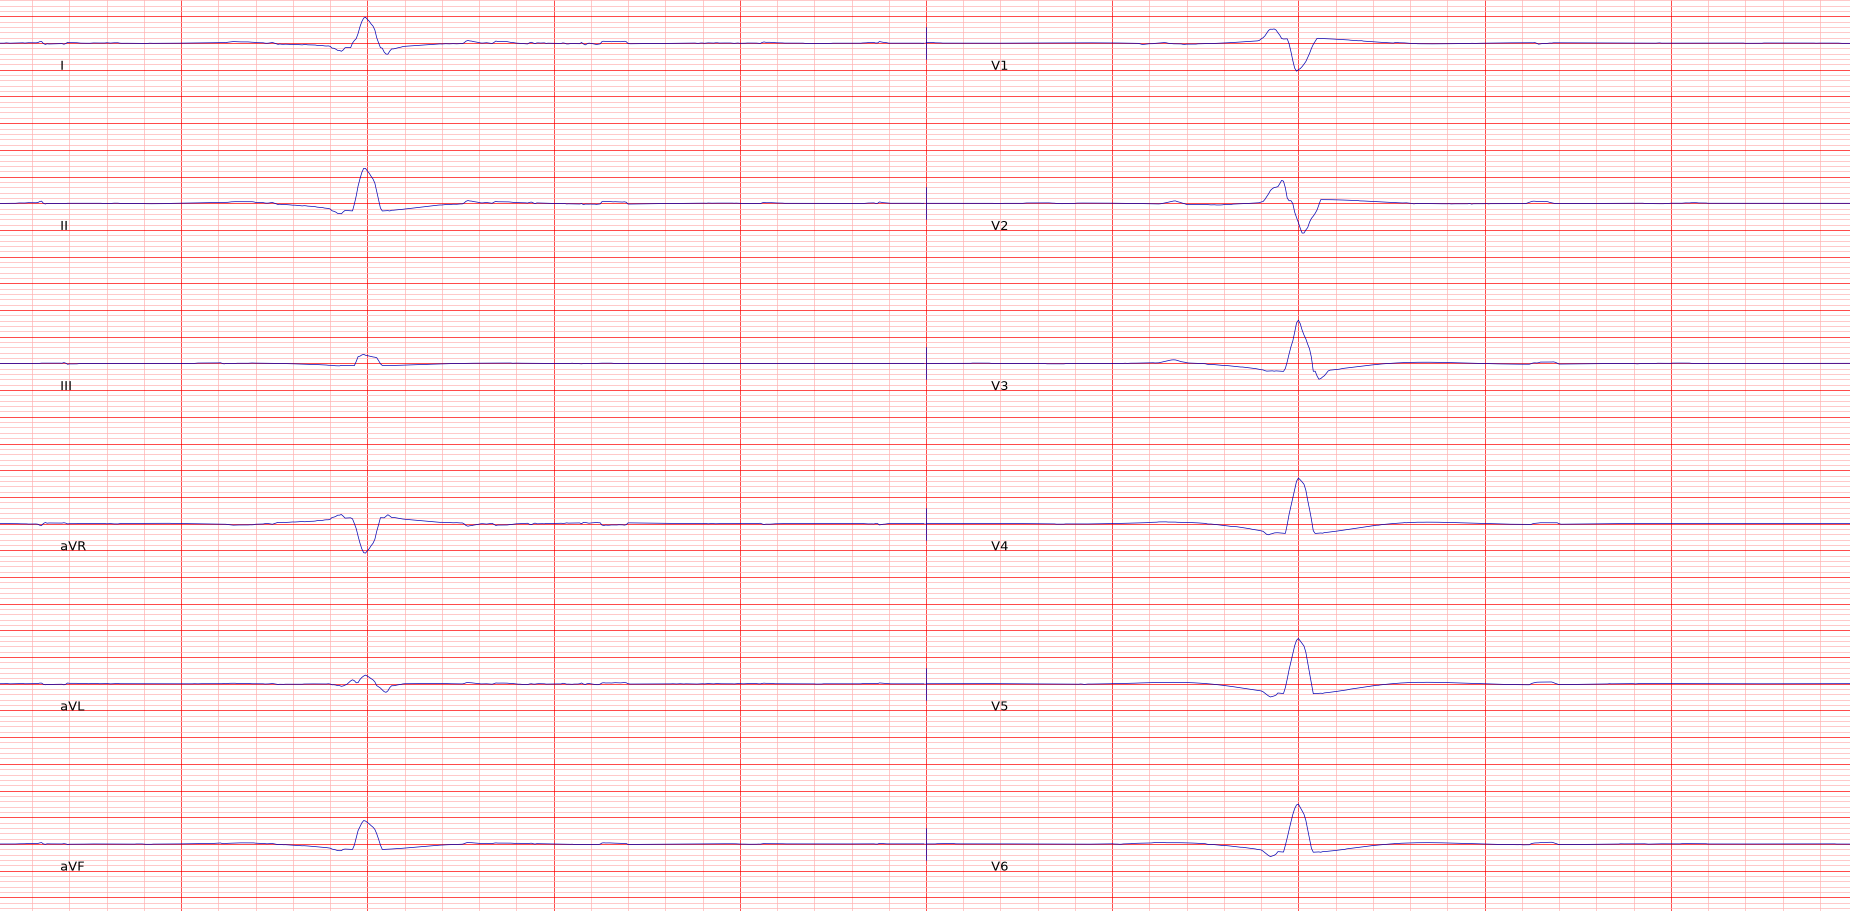
\includegraphics[width=\textwidth]{images/beat_segment.png}
	\caption{Finestra di segmentazione $[R-400\,\text{ms},\,R+600\,\text{ms}]$ centrata sul picco R, sovrapposta a un tracciato ECG di esempio.}
	\label{fig:finestra_segmentazione}
\end{figure}

La scelta di un'asimmetria tra la porzione precedente e quella successiva al picco R (400~ms prima, 600~ms dopo) è motivata dalla successione temporale delle componenti morfologiche dell'onda ECG all'interno di un singolo ciclo cardiaco:

\begin{itemize}
	\item i 400~ms che precedono il picco R sono sufficienti a includere l'onda P (depolarizzazione atriale) e il tratto PR, che hanno una durata tipica complessiva dell'ordine di circa 200~ms;
	\item i 600~ms successivi al picco R sono necessari a includere il resto del complesso QRS, il tratto ST e l'intera onda T (ripolarizzazione ventricolare), la cui durata complessiva, specialmente considerando l'intervallo QT, può arrivare fino a circa 400--450~ms in condizioni fisiologiche normali, con un margine di sicurezza per frequenze cardiache più basse (a cui corrisponde un intervallo QT più lungo).
\end{itemize}

Una finestra di un secondo, centrata in modo asimmetrico sul picco R, permette, nella grande maggioranza dei casi, di catturare un intero ciclo cardiaco (onda P, complesso QRS, onda T) senza includere porzioni significative del battito precedente o successivo, anche per frequenze cardiache elevate. Una finestra i cui estremi cadono fuori dai limiti della registrazione (tipicamente il primo o l'ultimo battito) viene scartata.

\subsection{Numero di battiti estratti: differenza tra train/val e test}
\label{sec:beat_count_per_split}

Il numero di battiti estratti da ciascuna registrazione dipende dallo split di appartenenza, poiché training/validazione e test hanno scopi diversi nella pipeline:

\begin{itemize}
	\item \textbf{Training e validazione}: da ogni registrazione vengono estratti esattamente \textbf{due battiti}: i primi e gli ultimi battiti di ciascuna registrazione di 10 secondi vengono deliberatamente evitati per eliminare l'influenza dei transitori di accensione, dei filtri analogici e degli effetti di bordo temporali introdotti dai filtri di preprocessing. La scelta del terzo e del quinto picco garantisce l'estrazione di cicli cardiaci stabili e interni alla registrazione tramite una procedura deterministica e riproducibile. Se una registrazione produce meno di cinque picchi R validi, essa viene scartata e registrata come tale (si veda la Sezione~\ref{sec:struttura_finale}). Questi due battiti sono poi la base su cui viene applicata la simulazione degli scambi di elettrodi (Sezione~\ref{sec:simulazione_misplacement}).
	\item \textbf{Test}: da ogni registrazione vengono estratti \textbf{tutti i battiti validi}, senza limitarsi a due. Questa scelta è funzionale alla strategia di valutazione adottata, poiché, in fase di test, ogni registrazione viene classificata tramite \emph{majority voting} sulle predizioni ottenute sui singoli battiti che la compongono, e disporre di più battiti per registrazione rende questa stima più robusta. I battiti di test non vengono sottoposti ad alcuna trasformazione e sono etichettati come ``normale'', poiché rappresentano registrazioni reali presumibilmente acquisite con un posizionamento corretto degli elettrodi.
\end{itemize}

\section{Simulazione degli scambi di elettrodi}
\label{sec:simulazione_misplacement}

\subsection{Perché è necessaria una simulazione}

I database di partenza, come la generalità dei database ECG pubblici, contengono esclusivamente registrazioni acquisite con un posizionamento corretto degli elettrodi: non esiste, nella pratica clinica, la produzione sistematica e su larga scala di registrazioni etichettate come ``mal posizionate'', poiché si tratta di un errore di acquisizione che, quando osservato, viene generalmente corretto immediatamente e non salvato. Per addestrare un modello supervisionato in grado di riconoscere queste condizioni, è quindi necessario disporre di esempi delle diverse classi di errore, e l'unica strada percorribile è la generazione artificiale di tali esempi a partire da registrazioni corrette. Questa simulazione viene applicata unicamente ai battiti di training e validazione (si veda la Sezione~\ref{sec:beat_count_per_split}); i battiti di test restano non trasformati.

Questo approccio è reso possibile dal fatto che il posizionamento errato di un elettrodo non introduce, dal punto di vista del segnale, un errore arbitrario, bensì un effetto ben determinabile e prevedibile, descrivibile a partire dalle equazioni che definiscono le derivazioni standard. È proprio questa proprietà che viene sfruttata per costruire la simulazione.

\subsection{Equazioni delle derivazioni standard}

Le sei derivazioni degli arti non sono misurate direttamente, ma calcolate a partire dai potenziali elettrici rilevati da tre elettrodi posizionati sugli arti: braccio destro (\textit{RA}, right arm), braccio sinistro (\textit{LA}, left arm) e gamba sinistra (\textit{LL}, left leg). Indicando con $V_{RA}$, $V_{LA}$, $V_{LL}$ i potenziali rilevati ai tre elettrodi, le tre derivazioni bipolari di Einthoven sono definite come:

\begin{align}
	I   &= V_{LA} - V_{RA} \\
	II  &= V_{LL} - V_{RA} \\
	III &= V_{LL} - V_{LA}
\end{align}

mentre le tre derivazioni aumentate unipolari di Goldberger sono definite come:

\begin{align}
	aVR &= V_{RA} - \frac{V_{LA} + V_{LL}}{2} = -\frac{I + II}{2}\\
	aVL &= V_{LA} - \frac{V_{RA} + V_{LL}}{2} = \frac{I-III}{2}\\
	aVF &= V_{LL} - \frac{V_{RA} + V_{LA}}{2} = \frac{II+III}{2}
\end{align}

Le sei derivazioni precordiali $V_1, \dots, V_6$ sono invece derivazioni unipolari riferite al \emph{terminale centrale di Wilson} (WCT), definito come la media dei tre potenziali degli arti:

\begin{equation}
	WCT = \frac{V_{RA} + V_{LA} + V_{LL}}{3}
\end{equation}

\subsection{Effetto di uno scambio di elettrodi}

Si consideri il caso in cui i cavi collegati agli elettrodi RA e LA vengano scambiati fisicamente. Il canale che l'elettrocardiografo ha registrato come ``RA'' riceve, in realtà, il potenziale dell'elettrodo posizionato sul braccio sinistro, e viceversa. Sostituendo $V_{RA} \to V_{LA}$ e $V_{LA} \to V_{RA}$ nelle equazioni precedenti, si ottiene un nuovo insieme di derivazioni, indicate con l'apice:

\begin{align}
	I' &= V_{RA} - V_{LA} = -(V_{LA}-V_{RA}) = -I \\
	II' &= V_{LL} - V_{LA} = III \\
	III' &= V_{LL} - V_{RA} = II \\
	aVR' &= V_{LA} - \frac{V_{RA}+V_{LL}}{2} = aVL \\
	aVL' &= V_{RA} - \frac{V_{LA}+V_{LL}}{2} = aVR \\
	aVF' &= V_{LL} - \frac{V_{RA}+V_{LA}}{2} = aVF
\end{align}

Le nuove derivazioni non sono altro che permutazioni delle derivazioni originali. In altre parole, è possibile ottenere il tracciato che si sarebbe osservato in caso di scambio RA--LA a partire da un tracciato acquisito correttamente, applicando esclusivamente operazioni algebriche lineari alle derivazioni già disponibili, senza dover disporre dei potenziali grezzi ai singoli elettrodi (che né PTB-XL né Georgia, come la generalità degli apparecchi clinici, forniscono). È esattamente questa proprietà che rende possibile, e corretta dal punto di vista elettrofisiologico, la simulazione degli scambi di elettrodi a partire dai soli dati disponibili.

Un'osservazione analoga si applica al terminale centrale di Wilson: poiché $WCT$ è una somma simmetrica dei tre potenziali agli arti, il suo valore non cambia se due di questi vengono scambiati tra loro:

\begin{equation}
	WCT' = \frac{V_{LA} + V_{RA} + V_{LL}}{3} = \frac{V_{RA} + V_{LA} + V_{LL}}{3} = WCT
\end{equation}

Ne consegue che le derivazioni precordiali $V_1$--$V_6$ non sono alterate da alcuno scambio tra gli elettrodi degli arti.

Applicando lo stesso procedimento agli altri due scambi possibili tra elettrodi degli arti (LA--LL e RA--LL), si ottengono le trasformazioni riportate in Tabella~\ref{tab:trasformazioni_scambio}.

\begin{table}[htbp!]
	\centering
	\caption{Trasformazioni delle derivazioni degli arti in funzione dello scambio di elettrodi simulato. Le derivazioni precordiali (V1--V6) restano invariate in tutti i casi.}
	\label{tab:trasformazioni_scambio}
	\begin{tabular}{@{}lllllll@{}}
		\toprule
		\textbf{Scambio} & $I'$ & $II'$ & $III'$ & $aVR'$ & $aVL'$ & $aVF'$ \\
		\midrule
		RA -- LA & $-I$   & $III$  & $II$   & $aVL$ & $aVR$ & $aVF$ \\
		LA -- LL & $II$   & $I$    & $-III$ & $aVR$ & $aVF$ & $aVL$ \\
		RA -- LL & $-III$ & $-II$  & $-I$   & $aVF$ & $aVL$ & $aVR$ \\
		\bottomrule
	\end{tabular}
\end{table}

Un caso ulteriore, più semplice, è lo scambio tra due cavi precordiali adiacenti, frequente nella pratica clinica per la vicinanza fisica degli elettrodi sul torace. In questo caso, poiché il terminale centrale di Wilson dipende esclusivamente dagli elettrodi degli arti e non dagli elettrodi precordiali, lo scambio si traduce semplicemente nello scambio diretto dei due canali coinvolti, lasciando invariate tutte le altre derivazioni. Il modulo di trasformazione implementa, in questa forma, tutti e cinque gli scambi tra derivazioni precordiali adiacenti (V1--V2, V2--V3, V3--V4, V4--V5, V5--V6), oltre ai tre scambi tra elettrodi degli arti (RA--LA, LA--LL, RA--LL) e alla classe ``normale'' (nessuna trasformazione), per un totale di nove trasformazioni disponibili, riassunte in Tabella~\ref{tab:trasformazioni_disponibili}. Ciascuna classe potrà essere associata ad un peso configurabile in fase di generazione del dataset.

\begin{table}[htbp]
	\centering
	\caption{Trasformazioni disponibili nel modulo di simulazione degli scambi di elettrodi.}
	\label{tab:trasformazioni_disponibili}
	\begin{tabular}{@{}ll@{}}
		\toprule
		\textbf{Nome} & \textbf{Tipo di scambio} \\
		\midrule
		\texttt{normal} & nessuno (identità) \\
		\texttt{RA\_LA} & elettrodi degli arti, braccio destro / braccio sinistro \\
		\texttt{LA\_LL} & elettrodi degli arti, braccio sinistro / gamba sinistra \\
		\texttt{RA\_LL} & elettrodi degli arti, braccio destro / gamba sinistra \\
		\texttt{V1\_V2} & precordiale adiacente \\
		\texttt{V2\_V3} & precordiale adiacente \\
		\texttt{V3\_V4} & precordiale adiacente \\
		\texttt{V4\_V5} & precordiale adiacente \\
		\texttt{V5\_V6} & precordiale adiacente \\
		\bottomrule
	\end{tabular}
\end{table}
\newpage
Va inoltre osservato che lo scambio tra l'elettrodo di massa/riferimento (\textit{RL}, right leg) e l'elettrodo \emph{LL} non è incluso tra le trasformazioni implementate, poiché, essendo in punti anatomicamente distanti dal cuore e \emph{isopotenziali}, i tracciati subirebbero alterazioni quasi impercettibili. Un altro motivo risiede nell'impossibilità di ricavare matematicamente il potenziale grezzo dell'elettrodo \emph{RL}.

La Figura~\ref{fig:scambio_RA_LA} mostra, a titolo esemplificativo, l'effetto della trasformazione RA--LA su un singolo battito segmentato, per un sottoinsieme delle derivazioni coinvolte: si osservi in particolare l'inversione di polarità della derivazione I e lo scambio di forma d'onda tra le derivazioni aVR e aVL.

\begin{figure}[htbp!]
	\centering
	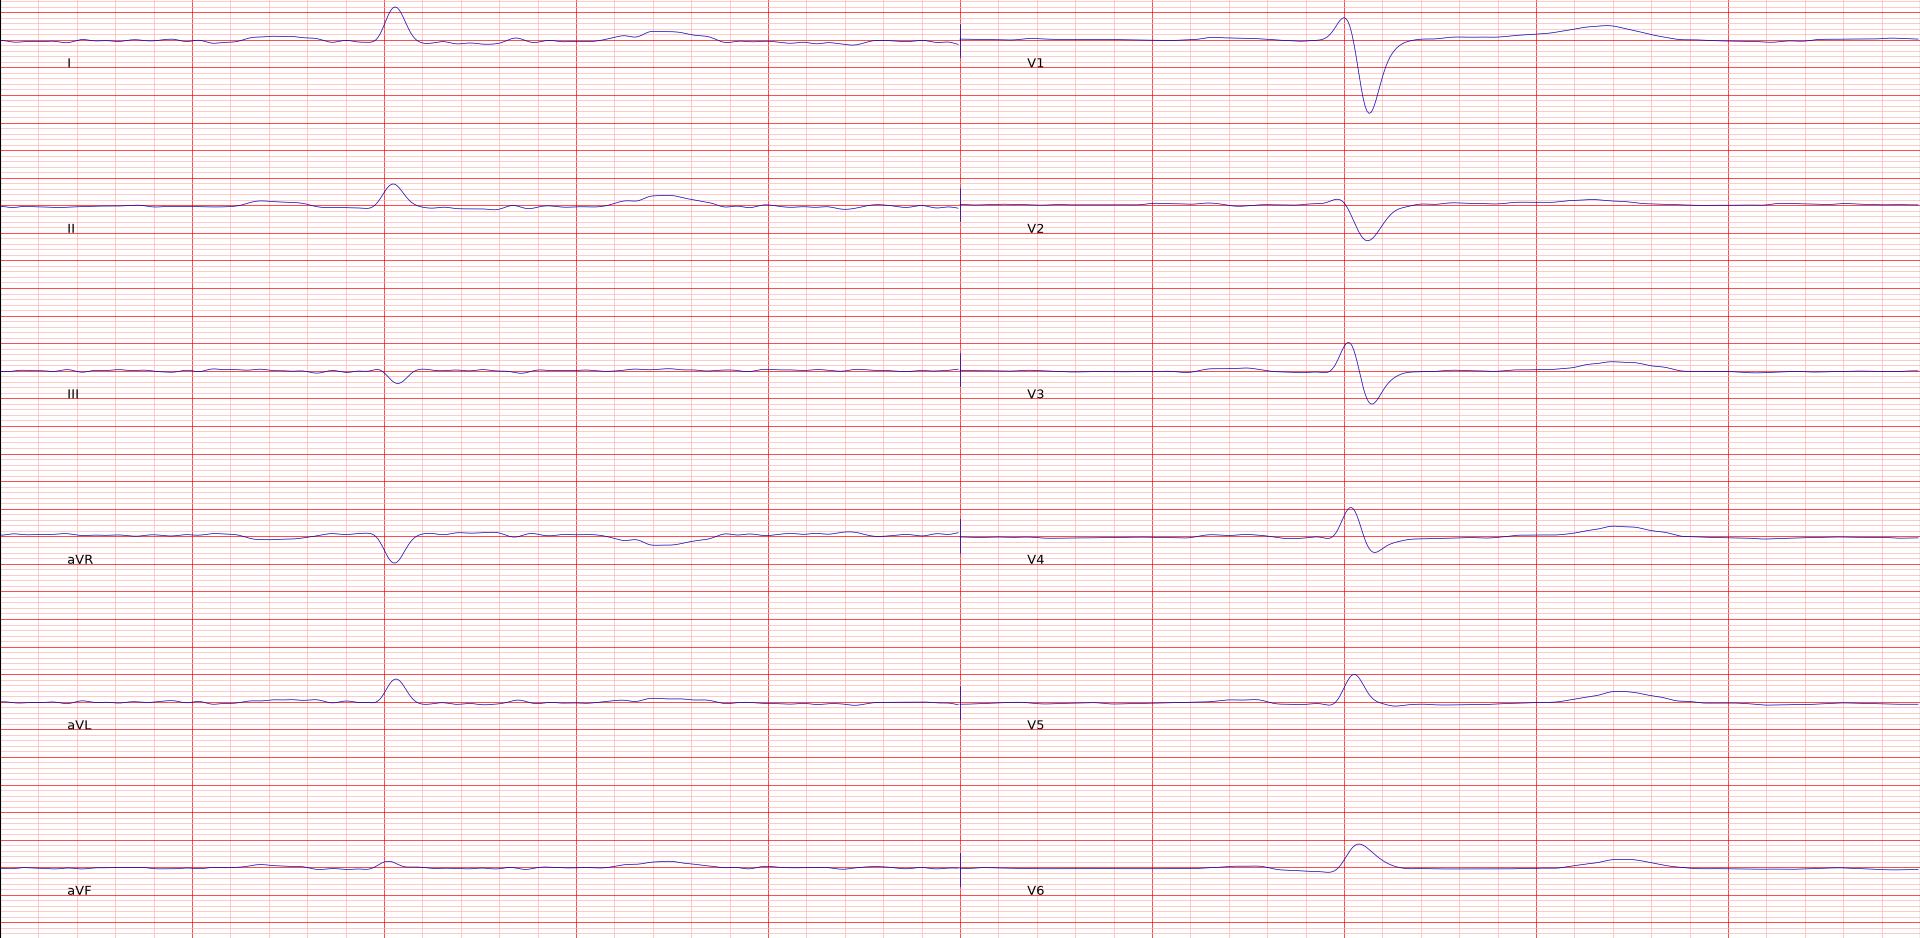
\includegraphics[width=\textwidth]{images/misplace_ecg.png}
	\caption{Battito trasformato secondo lo scambio RA--LA.}
	\label{fig:scambio_RA_LA}
\end{figure}
\newpage

\subsection{Regole di generazione del dataset finale}
\label{final_dataset}
L'applicazione pratica delle trasformazioni descritte sopra ai battiti segmentati segue alcune regole progettuali, motivate dalla necessità di produrre un dataset privo di possibili fonti di \emph{data leakage}. Tali regole si applicano ai soli split di training e validazione, gli unici in cui viene simulato il malposizionamento (si veda la Sezione~\ref{sec:beat_count_per_split} per il test).

\begin{enumerate}
	\item \textbf{I due battiti di ogni registrazione hanno etichette diverse.} Per ciascuna registrazione di training o validazione vengono estratti due segmenti, come descritto nella Sezione~\ref{beat-by-beat-segmentation}, e a ciascuno dei due viene assegnata un'etichetta diversa dall'altro, scelta tra ``normale'' e le diverse tipologie di scambio selezionate, secondo proporzioni configurabili. Questa scelta è motivata dal fatto che assegnare la stessa etichetta a entrambi i battiti di una stessa registrazione non aggiungerebbe reale informazione che la rete possa apprendere, finendo per appesantire la fase di training senza alcun guadagno.
	\item \textbf{Per ciascun battito viene mantenuta una sola versione.} Il dataset finale non contiene, per uno stesso segmento originale, sia la versione acquisita correttamente sia quella trasformata: viene conservata esclusivamente la versione corrispondente alla classe assegnata. In questo modo si evita di introdurre nel dataset coppie di esempi quasi identici (differenti unicamente per l'etichetta), che comprometterebbero la validità dello split e potrebbero facilitare un apprendimento per memorizzazione anziché per generalizzazione.
	\item \textbf{L'assegnazione delle classi avviene sull'insieme combinato PTB-XL + Georgia di ciascuno split.} Le etichette non vengono assegnate separatamente ai battiti dei due database, ma sull'unione di tutte le registrazioni PTB-XL e Georgia appartenenti allo stesso split (training o validazione): questo garantisce che le proporzioni tra classi richieste in fase di configurazione (ad esempio 50\% ``normale'' e il resto suddiviso equamente tra i quattro tipi di scambio) valgano sul dataset combinato effettivamente usato per addestrare il modello, e non separatamente sulle due sorgenti.
	\item \textbf{Lo split tra training, validazione e test è definito a monte, per paziente.} Come descritto nella Sezione~\ref{sec:split}, la suddivisione avviene prima della segmentazione ed è basata sull'identificativo di paziente: questo garantisce che tutti i battiti provenienti da uno stesso paziente appartengano a un unico insieme, evitando che il modello venga valutato su battiti provenienti da un paziente già osservato, seppur in forma diversa, durante l'addestramento.
\end{enumerate}

\section{Struttura del dataset finale}
\label{sec:struttura_finale}

Al termine della pipeline, il dataset è organizzato in tre sottocartelle separate, una per ciascuno split (\texttt{train/}, \texttt{val/}, \texttt{test/}), ciascuna con la stessa struttura interna:

\begin{itemize}
	\item una cartella \texttt{segments/}, contenente un file \texttt{.npy} per ciascun battito, con forma \texttt{(12, lunghezza\_finestra)}, cioè \emph{leads-first}, con le 12 derivazioni sulla prima dimensione, dove \texttt{lunghezza\_finestra} dipende dalla frequenza di campionamento scelta (500 campioni per una finestra di un secondo a \SI{500}{Hz}).
	\item un file di indice: \texttt{final\_dataset\_index.csv} per gli split di training e validazione, \texttt{beats\_index.csv} per lo split di test. In entrambi i casi, ogni riga corrisponde a un battito e riporta: il nome del file \texttt{.npy} corrispondente (\texttt{filename}); l'identificativo della registrazione di provenienza, prefissato con la sorgente (\texttt{ecg\_id}, ad es. \texttt{ptbxl\_1234} o \texttt{georgia\_E00001}); l'identificativo del paziente, anch'esso prefissato con la sorgente (\texttt{patient\_id}); il database di origine (\texttt{source}, \texttt{ptbxl} oppure \texttt{georgia}); la posizione del battito all'interno della registrazione (\texttt{beat\_idx\_in\_record}); il campione in cui è stato rilevato il picco R utilizzato per la segmentazione (\texttt{r\_peak\_sample}); e l'etichetta di classe (\texttt{label}: \texttt{normal} oppure il tipo di scambio simulato -- per il test, sempre \texttt{normal});
	\item un file \texttt{skipped\_records.csv}, che elenca le registrazioni scartate durante l'elaborazione di quello split, con il relativo motivo (ad esempio segnale contenente valori non definiti, numero di picchi R insufficiente, o errori di lettura/formato del file WFDB).
\end{itemize}

Questa struttura, oltre a facilitare il caricamento efficiente dei dati durante l'addestramento (ogni esempio può essere letto individualmente, senza necessità di caricare l'intero dataset in memoria), consente di ricostruire in ogni momento la provenienza di ciascun esempio, e mantiene traccia delle registrazioni escluse dalla pipeline, utile in fase di verifica della qualità del dataset. La distinzione tra i due file di indice (\texttt{final\_dataset\_index.csv} e \texttt{beats\_index.csv}) riflette inoltre la diversa natura dei due split: mentre train e validazione sono pensati per l'addestramento a livello di singolo battito, il test è organizzato per essere valutato a livello di intera registrazione tramite \emph{majority voting} su tutti i suoi battiti, aggregati tramite la colonna \texttt{ecg\_id}.

\section{Terzo database solo per il test}
\label{china_dataset}

Oltre allo split di test ricavato da PTB-XL e Georgia (Sezione~\ref{sec:beat_count_per_split}), le prestazioni del modello sono state valutate anche su un \textit{terzo database, indipendente e utilizzato esclusivamente per il test}, con l'obiettivo di verificare la capacità di generalizzazione su registrazioni provenienti da un contesto di acquisizione completamente diverso da quello visto in fase di addestramento (diversa popolazione, apparecchiatura e origine geografica).

Il database in questione, indicato nella repository del progetto come \emph{China database}, corrisponde all'\emph{ECG Arrhythmia Database} distribuita da PhysioNet~\cite{zheng2022ecgarrhythmia}, nota in letteratura anche come database Chapman--Shaoxing--Ningbo (CSN)~\cite{zheng2020chapman}. Si tratta di un database di ECG a 12 derivazioni raccolto in Cina, la cui popolazione, apparecchiatura di acquisizione e condizioni di registrazione differiscono sensibilmente da quelle di PTB-XL e Georgia.

\subsection{Preparazione dei dati}

Il database originale contiene 45\,152 registrazioni ECG. Durante la fase di preparazione, ogni registrazione è stata convertita in un insieme di segmenti con la stessa procedura di segmentazione descritta nella Sezione~\ref{beat-by-beat-segmentation} per lo split di test di PTB-XL e Georgia..

Delle 45\,152 registrazioni originali, 43\,712 sono state elaborate con successo, mentre 1\,440 sono state escluse a causa dell'assenza di picchi R rilevabili, di segmenti validi ai bordi del segnale, oppure di errori durante il caricamento o il preprocessing (le stesse categorie di scarto già introdotte per PTB-XL e Georgia nella Sezione~\ref{sec:struttura_finale}). Dalle registrazioni utilizzabili sono stati estratti complessivamente 445\,520 battiti. Le caratteristiche principali del database e i risultati della fase di preparazione sono riassunti nella Tabella~\ref{tab:china_caratteristiche}.

\begin{table}[htbp]
	\centering
	\caption{Caratteristiche principali del database utilizzato esclusivamente per il test (China)~\cite{zheng2022ecgarrhythmia, zheng2020chapman}.}
	\label{tab:china_caratteristiche}
	\begin{tabular}{@{}ll@{}}
		\toprule
		\textbf{Caratteristica} & \textbf{Valore} \\
		\midrule
		Numero di registrazioni ECG originali & 45\,152 \\
		Registrazioni elaborate con successo & 43\,712 \\
		Registrazioni escluse & 1\,440 \\
		Battiti estratti & 445\,520 \\
		Durata di ciascuna registrazione & 10 secondi \\
		Derivazioni & 12 \\
		Frequenza di campionamento & 500~Hz \\
		Formato dei segnali grezzi & WFDB \\
		Annotazioni diagnostiche & Codici SNOMED-CT \\
		Origine geografica & Cina (interferenza a \SI{50}{Hz}) \\
		Ruolo nella pipeline & solo test, nessuna trasformazione simulata \\
		\bottomrule
	\end{tabular}
\end{table}

\subsection{Utilizzo nella valutazione}

A differenza degli split di training e validazione, sui battiti estratti dal database China non è stata applicata alcuna trasformazione artificiale di malposizionamento, tutti i battiti sono etichettati come \texttt{normal}, coerentemente con l'assunzione, già discussa per PTB-XL e Georgia, che le registrazioni pubbliche disponibili siano state acquisite con un posizionamento corretto degli elettrodi.

Questa scelta consente di misurare sul database China, la capacità di generalizzare su un contesto di acquisizione mai osservato durante il training. Come per lo split di test di PTB-XL e Georgia, anche in questo caso la valutazione non è condotta a livello del singolo battito, ma le predizioni relative ai diversi segmenti appartenenti alla stessa registrazione vengono aggregate tramite \emph{majority voting}, ottenendo una predizione finale a livello di intera registrazione. Questa aggregazione riduce l'influenza di eventuali errori su singoli battiti isolati e permette di dare una migliore valutazione della capacità del modello di riconoscere la eventuali malposizionamenti.
%---------------CAPITOLO 5---------------

%---------------CAPITOLO 6---------------
\chapter{Architetture proposte}
\label{chap_6}
Lo stato dell'arte per la classificazione di varie patologie è l'utilizzo di algoritmi di deep learning; in questo capitolo tratteremo le tre architetture implementate nel presente lavoro di tesi: un \textbf{Multi-Layer Perceptron} (MLP), una \textbf{Convolutional Neural Network} (CNN) monodimensionale e una \textbf{Graph Convolutional Network} (GCN) con backbone convoluzionale. Le tre architetture vengono presentate in ordine di complessità crescente, sia dal punto di vista strutturale sia da quello delle formulazioni matematiche necessarie alla loro comprensione. Per ognuna, gli iperparametri specifici (numero di layer, numero di neuroni/filtri, dimensione dei kernel, ecc.) sono stati determinati tramite ottimizzazione bayesiana con \textbf{Optuna}, ripetuta separatamente per ciascuna configurazione del problema, in funzione del tipo di inversione degli elettrodi da rilevare e del numero di classi del task di classificazione considerato.

\section{Multi-Layer Perceptron}
\label{sec:mlp}

Il \textbf{Multi-Layer Perceptron} (MLP) rappresenta l'architettura più semplice tra quelle proposte ed è stato utilizzato come modello di baseline. Si tratta di una rete neurale \textit{feed-forward} completamente connessa (\textit{fully connected}), in cui ogni neurone di un layer riceve in ingresso l'output di tutti i neuroni del layer precedente. La rete è organizzata in un layer di ingresso, uno o più layer nascosti e un layer di uscita, la cui dimensione dipende dal numero di classi del problema di classificazione affrontato. Il numero di layer nascosti e il numero di neuroni per layer sono stati determinati tramite ottimizzazione con Optuna, in funzione della specifica configurazione del task.

\subsection{Funzioni di Attivazione}

Le \textbf{funzioni di attivazione} introducono non-linearità nella rete, permettendo al modello di apprendere relazioni complesse tra i dati in input. Senza di esse, indipendentemente dal numero di layer, la rete si comporterebbe come un semplice modello lineare.

Le funzioni di attivazione più comuni sono:

\begin{itemize}
	\item \textbf{ReLU (Rectified Linear Unit)}: definita come $f(x) = \max(0, x)$, azzera tutti i valori negativi e lascia invariati quelli positivi. È la funzione più utilizzata grazie alla sua semplicità computazionale e alla sua efficacia nel ridurre il problema del \textit{vanishing gradient}.
	\item \textbf{Sigmoid}: definita come $f(x) = \frac{1}{1 + e^{-x}}$, mappa i valori in un intervallo $(0, 1)$. Viene tipicamente usata nell'ultimo layer per problemi di classificazione binaria.
	\item \textbf{Softmax}: estensione della sigmoid per problemi multi-classe, produce una distribuzione di probabilità sull'insieme delle classi: $f(x_i) = \frac{e^{x_i}}{\sum_j e^{x_j}}$.
\end{itemize}

\subsection{Funzione di Loss}

La \textbf{loss function} (funzione di costo) quantifica l'errore tra le previsioni del modello $\hat{y}$ e i valori reali $y$ nel training set. L'obiettivo dell'apprendimento è minimizzare questa funzione.

Le loss function più utilizzate sono:

\begin{itemize}
	\item \textbf{Cross-Entropy Loss} (per classificazione multi-classe): misura la distanza tra la distribuzione predetta e quella reale.
	\[
	\mathcal{L} = -\sum_{c=1}^{C} y_c \log(\hat{y}_c)
	\]
	dove $C$ è il numero di classi, $y_c \in \{0,1\}$ è il label reale e $\hat{y}_c$ è la probabilità predetta per la classe $c$.
	
	\item \textbf{Mean Squared Error} (per regressione):
	\[
	\mathcal{L} = \frac{1}{N} \sum_{i=1}^{N} (y_i - \hat{y}_i)^2
	\]
\end{itemize}

\subsection{Fondamenta matematiche}
In questa sezione richiameremo alcuni strumenti di calcolo differenziale, necessari per la comprensione dell'aggiornamento dei pesi di una rete tramite l'\textbf{algoritmo di backpropagation}:

\subsubsection{Chain Rule}
La chain rule è la formula fondamentale per il calcolo della derivata di una funzione composta. Siano $g:\mathbb{R}\to\mathbb{R}$ e $f:\mathbb{R}\to\mathbb{R}$ derivabili, allora $g\circ f:\mathbb{R}\to\mathbb{R}$ è anch'essa derivabile, e se poniamo $h(x)=g(f(x))$, abbiamo che:
\[
\frac{dh}{dx}=g'(f(x))\cdot f'(x)
\]
Espandendo il ragionamento, definiamo $q:\mathbb{R}\to\mathbb{R}$; allora $q\circ g\circ f:\mathbb{R}\to\mathbb{R}$ è derivabile, e ridefinendo $h(x)=q(g(f(x)))$ otteniamo:
\[
\frac{dh}{dx}=q'(g(f(x)))\cdot g'(f(x))\cdot f'(x)
\]

\subsubsection{Chain rule per funzioni di funzioni}

Consideriamo un vettore $x(t)=\big(x_1(t),x_2(t),\dots, x_n(t)\big)^T\in\mathbb{R}^n$, le cui componenti sono $n$ funzioni derivabili. Sia inoltre $f:\mathbb{R}^n \to\mathbb{R}$ una funzione differenziabile in $x(t)$.

Sotto queste ipotesi, la funzione composta $F(t) = f(x(t))$ risulta differenziabile in $t$, e la sua derivata si esprime attraverso la chain rule come:
\[
F'(t)=\sum_{i=1}^{n}\frac{\partial f(x(t))}{\partial x_i} \cdot x_i'(t)=\langle\nabla f(x(t)),x'(t)\rangle
\]
dove l'espressione finale denota il prodotto scalare tra il gradiente della funzione $f$ e il vettore derivato $x'(t)$.

A titolo di esempio, data una funzione che dipende da due componenti generiche, ovvero $f\big(h(t), g(t)\big)$, la derivata totale di $f$ rispetto al parametro $t$ si calcola come:
\[
\frac{df}{dt} = \frac{\partial f}{\partial h} \frac{dh}{dt} + \frac{\partial f}{\partial g} \frac{dg}{dt}
\]

\subsubsection{Gradiente}
Sia $A\subseteq\mathbb{R}^2$ aperto e $f:A\to\mathbb{R}$, se tutte le derivate parziali esistono e sono continue allora $f$ è differenziabile. Se $f$ è differenziabile allora le sue derivate parziali, (due in questo caso) in un punto $P$ arbitrario, formano un vettore chiamato gradiente:
\[
\nabla f(x_0,y_0)=\left[\frac{\partial f}{\partial x}(x_0,y_0)\,, \quad\frac{\partial f}{\partial y}(x_0,y_0)\right]
\]

\subsubsection{Derivata direzionale}
Sia $A\subseteq\mathbb{R}^2$ aperto e $f:A\to\mathbb{R}$ continua, definiamo la derivata direzionale $D_v$ come la variazione della funzione $f$ lungo la direzione di un \textbf{versore} $v$ a partire da un punto $P$ arbitrario; viene formalmente indicata come:
\[
D_vf(x_0,\,y_0)=\lim_{t\to 0}\frac{f(x_0+t\,v_x,\,y_0+t\,v_y)-f(x_0,\,y_0)}{t}
\]
Se $f$ è anche \textbf{differenziabile}, allora possiamo ricorrere al \textbf{Teorema del Gradiente} per calcolare la derivata direzionale:
\[
D_vf(x_0,\,y_0)=\nabla f(x_0,\,y_0)\cdot v
\]
Espandendo otteniamo:
\[
\left[\frac{\partial f}{\partial x}(x_0,y_0)\,, \quad\frac{\partial f}{\partial y}(x_0,y_0)\right]\cdot \def\arraystretch{1.0} \begin{pmatrix}
	v_x \\ v_y
\end{pmatrix}
\]
Ora vogliamo calcolare qual'è la direzione $v$ in cui $f$ ha crescita massima:
\[
D_vf(x_0,\,y_0)=||\nabla f(x_0,\,y_0)||\cdot||v||\cdot\cos(\alpha)
\]
dove $\alpha$ indica l'angolo tra il versore e il gradiente. Osservando che $||v||=1$ e $-1\le\cos(\alpha)\le 1$ possiamo dire che $D_vf(x_0,\,y_0)$ assume valore \textbf{massimo} quando $\cos(\alpha)=1\to\alpha=0$, cioè se $v$ ha stessa direzione e verso del gradiente; viceversa assume valore \textbf{minimo} quando $\cos(\alpha)=-1\to\alpha=\pi$, cioè quando $v$ ha stessa direzione ma verso opposto al gradiente.

\subsection{Algoritmo di Backpropagation}
Uno dei primi algoritmi proposti per il calcolo dei pesi in una rete neurale è il metodo iterativo noto come metodo di backpropagation. La riscoperta di questo metodo verso la metà degli anni '80 da parte di Rumelhart, Hinton e Williams ha reso possibile definire algoritmi di addestramento per reti multistrato, ed è stato quindi alla base del successivo sviluppo degli studi sulle reti neurali. L'algoritmo è legato essenzialmente alla tecnica utilizzata per il calcolo delle derivate della funzione di errore, basata sulle regole di derivazione delle funzioni composte.

\subsubsection{Percorso generale di esecuzione}

Prima di tutto, è necessario definire come \textbf{epoca} il compimento di una fase di training, cioè quando tutto il dataset di training è passato attraverso la rete. Il dataset di training viene suddiviso in piccoli \emph{batch} (dimensione 16, 32, 64 ecc.), per ognuno si procede con il calcolo della funzione di loss $L(y, \hat{y})$, per poi proseguire con il calcolo della funzione di costo:
\[
C(w)=\frac{1}{n_T}\sum_{j=1}^{n_T}L(y^{(j)},\hat{y}^{(j)}(w))
\]
dove $n_T$ rappresenta la dimensione del batch di training, e $y^{(j)},\hat{y}^{(j)}$ sono rispettivamente le etichette e le predizioni della rete al $j$-esimo esempio di training.
Infine dobbiamo aggiornare i pesi muovendoci in direzione dell'antigradiente per cercare di minimizzare la funzione di costo:
\[
w^{(k)}=w^{(k-1)}-\eta\nabla C(w)
\]
dove $\eta$ rappresenta il \textbf{learning rate} (tasso di apprendimento) che definisce di quanto dobbiamo muoverci verso la direzione dell'antigradiente; questo parametro è fondamentale per l'apprendimento delle reti, in quanto, con valori troppo piccoli, la convergenza della rete richiederebbe tempi troppo lunghi, quindi più energia consumata e più epoche, mentre valori troppo grandi potrebbero evitare che la rete converga, in quanto i punti di minimo che cerchiamo di ottenere potrebbero essere "saltati" direttamente.

\begin{figure}[h!]
	\centering
	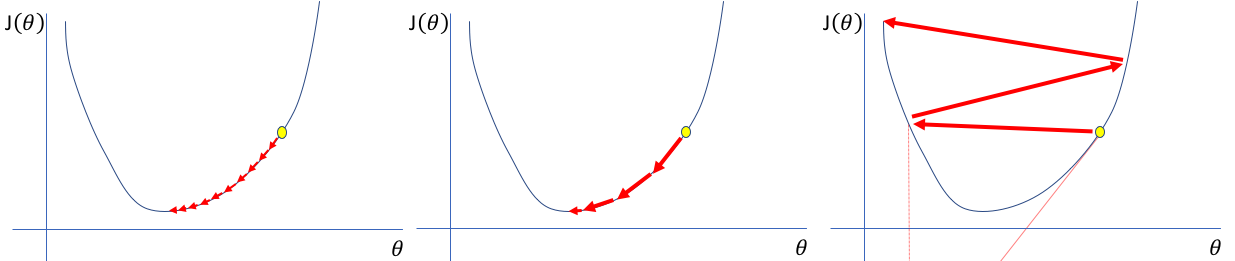
\includegraphics[width=0.9\linewidth]{images/lr_high_and_low.png}
	\caption{Differenza nella scelta del learning rate}
	\label{fig:lr_diff}
\end{figure}

\subsection{Calcolo del Gradiente in un MLP}

L'obiettivo della backpropagation è calcolare le derivate parziali della funzione di loss $L$ rispetto a ciascun peso della rete, così da poterli aggiornare tramite la discesa del gradiente. In un MLP, ogni neurone $i$ del layer $\ell$ riceve in ingresso una combinazione lineare degli output del layer precedente:
\[
a_i^{(\ell)}=\sum_jw_{ji}^{(\ell)}\,z_j^{(\ell-1)}+ b_i^{(\ell)}
\]
e produce in uscita il valore attivato:
\[
z_i^{(\ell)}=f\!\left(a_i^{(\ell)}\right)
\]
dove $f$ è la funzione di attivazione e $z_j^{(\ell-1)}$ è l'output del $j$-esimo neurone del layer precedente.

\subsubsection{Gradiente rispetto ai pesi}

Applicando la chain rule, la derivata parziale della loss rispetto al peso $w_{ji}^{(\ell)}$ che connette il neurone $j$ del layer $\ell-1$ al neurone $i$ del layer $\ell$ è:
\[
\frac{\partial L}{\partial w_{ji}^{(\ell)}}= \frac{\partial L}{\partial a_i^{(\ell)}}\cdot \frac{\partial a_i^{(\ell)}}{\partial w_{ji}^{(\ell)}}=\delta_i^{(\ell)}\cdot z_j^{(\ell-1)}
\]
dove abbiamo definito il \textbf{segnale di errore} $\delta$ del neurone $i$ al layer $\ell$ come:
\[
\delta_i^{(\ell)}=\frac{\partial L}{\partial a_i^{(\ell)}}
\]
Il gradiente rispetto a un peso è quindi il semplice prodotto tra il delta del neurone di destinazione e l'output del neurone sorgente.

\subsubsection{Calcolo del segnale di errore}

Il calcolo di $\delta_i^{(\ell)}$ dipende dalla posizione del neurone nella rete.

\paragraph{Layer di uscita.}
Se il neurone $i$, con $i = 1, \ldots, k$, appartiene al layer di uscita $L$, il delta si calcola direttamente derivando la loss rispetto alla preattivazione tramite la chain rule:
\[
\delta_i^{(L)} = \frac{\partial L(\hat{y}_i)}{\partial a_i^{(L)}} = f'\!\left(a_i^{(L)}\right) \frac{\partial L(\hat{y}_i)}{\partial \hat{y}_i}
\]
Il primo fattore è la derivata della funzione di attivazione valutata nella preattivazione, il secondo è la derivata della loss rispetto all'output predetto $\hat{y}_i=z_i^{(L)}$.

\paragraph{Layer nascosto.}
Se il neurone $i$, con $i = 1, \ldots, k$, appartiene a un layer nascosto $\ell$, il suo output $z_i^{(\ell)}$ contribuisce alla preattivazione di \emph{tutti} i neuroni del layer successivo. Applicando la chain rule su tutti questi percorsi:
\[
\delta_i^{(\ell)} = \frac{\partial L}{\partial a_i^{(\ell)}} = f'\!\left(a_i^{(\ell)}\right) \sum_{k=0}^{N^{(\ell+1)}} \delta_k^{(\ell+1)}\, w_{ik}^{(\ell+1)}
\]
dove $N^{(\ell)}$ è il numero di neuroni nel layer $\ell$ e la somma accumula i contributi di errore provenienti da tutti i neuroni del layer successivo, pesati dai rispettivi pesi. Questa formula permette di \textbf{propagare il segnale di errore all'indietro}, dal layer di uscita verso i layer più profondi, senza dover ricalcolare la loss da zero ad ogni passo.

\subsubsection{Vettore del gradiente e aggiornamento dei pesi}

Raccogliendo le derivate parziali rispetto a tutti i pesi del layer $\ell$ si ottiene il \textbf{gradiente} della loss rispetto alla matrice dei pesi $W^{(\ell)}$:
\[
\nabla_{W^{(\ell)}}L=\Delta^{(\ell)}\otimes Z^{(\ell-1)}
\]
dove $\Delta^{(\ell)}\in\mathbb{R}^{N^{(\ell)}}$ è il vettore dei delta del layer $\ell$ e $Z^{(\ell-1)}\in\mathbb{R}^{N^{(\ell-1)}}$ è il vettore degli output del layer precedente; $\otimes$ indica il prodotto esterno tra i due vettori, che produce una matrice di dimensione $N^{(\ell)}\times N^{(\ell-1)}$. Ogni elemento $(i,j)$ di questa matrice è esattamente $\delta_i^{(\ell)}\cdot z_j^{(\ell-1)}$.

I pesi vengono quindi aggiornati tramite la discesa del gradiente:
\[
W^{(\ell)}=W^{(\ell)}-\eta\,\nabla_{W^{(\ell)}} L
\]
dove $\eta$ è il learning rate. L'algoritmo procede layer per layer, dall'uscita verso l'ingresso, calcolando prima i delta tramite la formula ricorsiva e poi aggiornando i pesi con il gradiente corrispondente.

\section{Convolutional Neural Network}
\label{sec:cnn}

Le \textbf{Convolutional Neural Network} (CNN) sono una classe di reti neurali ispirate al funzionamento della corteccia visiva dei mammiferi. Nascono con l'idea di processare immagini e, a differenza delle reti neurali completamente connesse (MLP) descritte nella sezione precedente, le CNN non prevedono l'utilizzo di un neurone per ogni pixel, ma organizzano i neuroni stessi in tre dimensioni così da creare una serie di matrici chiamate \textbf{kernel} o \textbf{filtri}. Questo le rende particolarmente efficaci nell'estrazione automatica di feature da dati strutturati, come il segnale ECG monodimensionale considerato nel presente lavoro.

Come per l'MLP, l'apprendimento della rete avviene tramite la minimizzazione di una \textbf{loss function} (Cross-Entropy per la classificazione multi-classe, si veda la Sezione~\ref{sec:mlp}), utilizzando le medesime funzioni di attivazione (ReLU, Sigmoid, Softmax) e lo stesso algoritmo generale di \textbf{backpropagation} basato sulla chain rule. Ciò che cambia sostanzialmente rispetto all'MLP è la natura delle operazioni svolte da ciascun layer, che vedremo nel dettaglio in questa sezione.

Anche per la CNN, il numero di layer convoluzionali, il numero di filtri per layer, la dimensione dei kernel e la presenza/dimensione dei layer di pooling sono stati determinati tramite ottimizzazione con Optuna, in funzione della specifica configurazione del task di classificazione.

\subsection{Architettura di una CNN}

\subsubsection{Processo di convoluzione}

Il \textbf{convolutional layer} è il componente principale di una CNN. Esso ha il compito di applicare tutti i kernel all'immagine in input tramite l'operazione di \textbf{convoluzione discreta}. Dato un input $I\in\mathbb{R}^{H\times W\times C}$ e un kernel $K\in\mathbb{R}^{m\times n}$, l'elemento in posizione $(i,j)$ della matrice di output, chiamata \textbf{feature map}, è calcolato come:

\[
(I * K)(i, j) = \sum_{k=0}^{m-1} \sum_{l=0}^{n-1} I(i+k,\, j+l) \cdot K(k, l)
\]

Il filtro scorre sull'input con un passo definito dallo \textbf{stride}. Ogni filtro ha una quantità di pesi pari a $m\cdot n$ e sono condivisi su tutta l'immagine: questa proprietà, chiamata \textbf{weight sharing}, riduce drasticamente il numero di parametri rispetto a un layer completamente connesso e permette di apprendere feature locali indipendentemente dalla loro posizione.

Il risultato del layer convoluzionale è un insieme di feature map, una per ogni filtro applicato, che vengono poi passate alla funzione di attivazione.

\subsubsection{Pooling Layer}

I \textbf{pooling layer} hanno il compito di ridurre la dimensione spaziale delle feature map, rendendo la rete più efficiente e meno sensibile a piccole traslazioni dell'input (\textbf{invarianza traslazionale}).

Il tipo più comune è il \textbf{max pooling}: per ogni regione di dimensione $k \times k$ dell'input, viene selezionato il valore massimo. Un'alternativa è l'\textbf{average pooling}, che calcola la media dei valori nella regione. Il pooling non introduce nuovi parametri da apprendere, ma contribuisce a rendere le rappresentazioni più compatte e robuste.

\subsection{Calcolo del gradiente in una CNN}

A differenza di un MLP, in una CNN la struttura dei layer non è completamente connessa: i pesi dei filtri sono \textbf{condivisi} su tutta la mappa di attivazione (weight sharing) e le operazioni fondamentali sono convoluzioni, non semplici prodotti scalari. Per questo motivo, pur seguendo lo stesso principio generale della backpropagation basata sulla chain rule visto per l'MLP, il calcolo del gradiente differisce sostanzialmente tra le due architetture.

\subsubsection{Struttura delle variabili}

In un layer convoluzionale $\ell$, l'input non è un vettore, ma un \textbf{tensore} a tre dimensioni $Z^{(\ell-1)}\in\mathbb{R}^{H\times W\times C}$, dove $H$ e $W$ sono le dimensioni spaziali e $C$ è il numero di canali (o feature map). Il kernel è anch'esso un tensore $K^{(\ell)} \in\mathbb{R}^{m\times n\times C}$, con $m\times n$ dimensioni spaziali. L'output del layer convoluzionale, prima della funzione di attivazione, è la \textbf{feature map}:
\[
A^{(\ell)}_{ij}=\sum_{p=0}^{m-1}\sum_{q=0}^{n-1}\sum_{c=0}^{C-1}K^{(\ell)}_{pqc}\cdot Z^{(\ell-1)}_{i+p,\,j+q,\,c}+b^{(\ell)}
\]
dove $(i,j)$ è la posizione spaziale nella feature map di output e $b^{(\ell)}$ è il bias. Dopo l'applicazione della funzione di attivazione $f$, si ottiene:
\[
Z^{(\ell)}_{ij}=f\!\left(A^{(\ell)}_{ij}\right)
\]

\subsubsection{Segnale di errore nel layer convoluzionale}

Per un layer convoluzionale $\ell$, il \textbf{segnale di errore} $\delta$ associato alla posizione $(i,j)$ è definito, analogamente al caso MLP, come la derivata parziale della loss rispetto alla preattivazione:
\[
\delta^{(\ell)}_{ij}=\frac{\partial L}{\partial A^{(\ell)}_{ij}}
\]

Se il layer $\ell$ è un \textbf{layer nascosto}, come avviene per tutti i layer convoluzionali, il delta deve tener conto di come ogni preattivazione $A^{(\ell)}_{ij}$ contribuisce a \textbf{tutte} le posizioni della feature map del layer successivo. Per la chain rule:
\[
\delta^{(\ell)}_{ij}=f'\!\left(A^{(\ell)}_{ij}\right) \cdot\sum_{s}\sum_{t}\delta^{(\ell+1)}_{st}\cdot K^{(\ell+1)}_{i-s,\,j-t}
\]
L'operazione di somma pesata sui delta del layer successivo corrisponde a una \textbf{convoluzione} tra $\delta^{(\ell+1)}$ e il kernel $K^{(\ell+1)}$ ruotato di $180°$:
\[
\delta^{(\ell)}_{ij} = f'\!\left(A^{(\ell)}_{ij}\right) \cdot\left(\delta^{(\ell+1)}*\mathrm{rot}_{180}\!\left(K^{(\ell+1)}\right)\right)_{ij}
\]
La rotazione di $180^{\circ}$ del kernel è una conseguenza diretta della chain rule applicata all'operazione di convoluzione: ogni peso $K_{pq}$ ha contribuito alla preattivazione in posizione $(i,j)$ tramite l'input nella posizione $(i+p, j+q)$, quindi il segnale di errore deve essere distribuito nella direzione opposta.

\subsubsection{Gradiente rispetto ai pesi del filtro}

Il gradiente della funzione di loss rispetto a un singolo peso $K^{(\ell)}_{pq}$ del kernel si calcola tramite la chain rule, sommando il contributo di tutte le posizioni $(i,j)$ in cui quel peso è stato usato durante la convoluzione (\textit{weight sharing}):
\[
\frac{\partial L}{\partial K^{(\ell)}_{pq}}= \sum_{i}\sum_{j}\delta^{(\ell)}_{ij}\cdot Z^{(\ell-1)}_{i+p,\,j+q}
\]
Questa espressione è una \textbf{cross-correlazione} tra il segnale di errore $\delta^{(\ell)}$ e la feature map di input $Z^{(\ell-1)}$. A differenza del MLP, in cui il gradiente rispetto a un peso è il semplice prodotto $\delta_i^{(\ell)} \cdot z_j^{(\ell-1)}$, qui è necessario sommare su tutte le posizioni spaziali a causa del weight sharing: lo stesso peso $K_{pq}$ ha partecipato al calcolo di ogni elemento della feature map di output, quindi tutti questi contributi devono essere accumulati.

In forma vettoriale compatta, l'intero gradiente del kernel si scrive come:
\[
\nabla_{K^{(\ell)}}L=\delta^{(\ell)}\star Z^{(\ell-1)}
\]
dove $\star$ indica l'operazione di cross-correlazione tra le due matrici.

\subsubsection{Gradiente rispetto al bias}

Il gradiente rispetto al bias $b^{(\ell)}$ è la somma di tutti i delta del layer corrente su tutte le posizioni spaziali, poiché il bias è addizionato in ogni posizione:
\[
\frac{\partial L}{\partial b^{(\ell)}}= \sum_{i}\sum_{j}\delta^{(\ell)}_{ij}
\]

\subsubsection{Backpropagation attraverso il Pooling Layer}

Il pooling layer non contiene pesi da apprendere, ma è comunque necessario propagare il segnale di errore attraverso di esso. Nel caso del \textbf{max pooling}, durante il forward pass viene memorizzata la posizione del valore massimo in ogni regione $k\times k$ (\textit{argmax}). Nella backprop, il delta viene assegnato esclusivamente all'elemento che aveva valore massimo, mentre tutti gli altri ricevono un contributo nullo:
\[
\delta^{(\ell)}_{ij}=
\begin{cases}
	\delta^{(\ell+1)}_{\lfloor i/k\rfloor,\,\lfloor j/k\rfloor}&\text{se }(i,j)\text{ era il massimo nella sua regione} \\
	0&\text{altrimenti}
\end{cases}
\]
Nel caso dell'\textbf{average pooling}, il delta viene distribuito uniformemente su tutti gli elementi della regione:
\[
\delta^{(\ell)}_{ij} =\frac{1}{k^2}\,\delta^{(\ell+1)}_{\lfloor i/k\rfloor,\,\lfloor j/k\rfloor}
\]

\subsubsection{Aggiornamento dei pesi}

Una volta calcolati i gradienti per ogni layer, i pesi vengono aggiornati tramite la stessa regola di discesa del gradiente vista per l'MLP:
\[
K^{(\ell)}=K^{(\ell)}-\eta\,\nabla_{K^{(\ell)}}L \qquad b^{(\ell)}=b^{(\ell)}-\eta\,\frac{\partial L}{\partial b^{(\ell)}}
\]
dove $\eta$ è il learning rate. La struttura generale dell'algoritmo rimane quindi invariata rispetto al MLP; ciò che cambia è la \textbf{natura delle operazioni}: somme pesate scalari diventano cross-correlazioni e convoluzioni, dovuto alla geometria dei layer convoluzionali.

\subsection{CNN applicate a segnali monodimensionali}

Le CNN nascono per l'elaborazione di immagini bidimensionali, ma il loro meccanismo convoluzionale si può generalizzare a segnali monodimensionali come le serie temporali. Nel caso 1D, il filtro convoluzionale scorre lungo l'asse temporale anziché sullo spazio bidimensionale dell'immagine.

\subsubsection{Convoluzione 1D}

In una convoluzione 1D, abbiamo sempre il tensore $\mathbf{Z}\in\mathbb{R}^{H\times W\times C}$, ma il parametro $H$ ha valore uno, mentre $C$ dipende dai canali in ingresso, dodici nel nostro caso; i filtri seguono la stessa logica $\mathbf{K}\in\mathbb{R}^{n\times m\times C}\to\mathbf{K}\in\mathbb{R}^{n\times C}$. L'operazione di convoluzione 1D produce sempre una feature map preattivata $\mathbf{A}$ definita come:
\[
A_i^{(\ell)}=\sum_{j=0}^{n-1}Z_{i+j}^{(\ell-1)}\cdot K_j^{(\ell)}+b^{(\ell)}\xrightarrow{attivazione}Z_i^{(\ell)}=f\left(A_i^{(\ell)}\right)
\]
dove $b$ è il bias e $i$ scorre lungo la dimensione temporale. Estendendo a $N$ filtri, si ottengono $N$ feature map in uscita, ognuna specializzata nel rilevare un pattern morfologico diverso. Il segnale di errore $\delta$ si indica allo stesso modo, il calcolo invece risulta più semplice:
\[
\delta_i^{(\ell)}=\frac{\partial L}{\partial A_i^{(\ell)}}=f^{'}\left(A_i^{(\ell)}\right)\cdot \sum_j\delta^{(\ell+1)}_j\cdot K^{(\ell+1)}_{i-j}
\]
questa operazione può essere semplificata esattamente come spiegato nella sezione precedente:
\[
\delta^{(\ell)}_i=f^{'}\left(A^{(\ell)}_i\right)\cdot \left(\delta^{(\ell+1)}*rot_{180^{\circ}}\left(K^{(\ell +1)}\right)\right)_i
\]

\subsection{Vantaggi per i segnali ECG}

L'applicazione delle CNN 1D ai segnali ECG offre numerosi vantaggi rispetto agli approcci tradizionali basati su feature engineering manuale:

\begin{itemize}
	\item \textbf{Estrazione automatica delle feature}: la rete apprende autonomamente quali caratteristiche morfologiche (ampiezza e durata dell'onda P, complesso QRS, onda T, intervallo ST) sono discriminative per ogni classe, senza richiedere conoscenze a priori.
	
	\item \textbf{Invarianza locale}: grazie al pooling, la rete risulta robusta a piccole variazioni nella posizione temporale dei componenti del battito.
	
	\item \textbf{Gerarchia di rappresentazione}: i primi livelli convoluzionali apprendono pattern di basso livello (variazioni locali della forma d'onda), mentre i livelli più profondi combinano queste informazioni in rappresentazioni di alto livello (morfologie patologiche complesse).
	
	\item \textbf{Efficienza computazionale}: la condivisione dei pesi riduce il numero di parametri rispetto a una rete fully connected applicata allo stesso segnale.
\end{itemize}

\section{Graph Convolutional Network con CNN Backbone}
\label{sec:gcn}

L'ultima e più complessa architettura proposta è una \textbf{Signed Graph Convolutional Network} che utilizza una CNN 1D, analoga a quella descritta nella Sezione~\ref{sec:cnn}, come \textbf{backbone} per l'estrazione delle feature da ciascuna delle 12 derivazioni del segnale ECG. A differenza della CNN standard, dove le 12 derivazioni sono trattate come canali di un unico tensore di input, in questa architettura la backbone elabora ciascuna derivazione \emph{singolarmente e con pesi condivisi}, producendo un vettore di feature per ciascun nodo del grafo; è poi lo strato di \textit{message passing} a modellare esplicitamente come queste rappresentazioni si relazionano tra le diverse derivazioni, sfruttando una topologia di grafo \textbf{firmata (signed)} costruita a partire dalla geometria delle derivazioni.

Anche in questo caso, il numero di layer di message passing, la dimensione delle feature nodali e nascoste, il tipo di classificatore finale (lineare o MLP) e la scelta tra message passing signed o basato su attenzione sono stati determinati tramite ottimizzazione con Optuna, in funzione della configurazione specifica del task.

\subsection{Estrazione delle feature nodali: la CNN Backbone}
\label{sec:lead_cnn_encoder}

Ogni segmento ECG in ingresso ha dimensione $(12, T)$, con $T=500$ campioni corrispondenti a una finestra di un secondo campionata a $500\,\text{Hz}$ centrata sul picco dell'onda R. Prima che il grafo venga costruito, ciascuna delle 12 derivazioni viene elaborata \textbf{singolarmente} da una CNN 1D condivisa (\textit{LeadCNNEncoder}), che produce per ogni derivazione un vettore di feature di dimensione fissata $d_{\text{node}}$. Essendo i pesi condivisi tra tutte le derivazioni, la rete apprende pattern morfologici generici (onda P, complesso QRS, onda T) indipendentemente dalla derivazione specifica; sarà poi il layer di message passing a modellare come queste feature si relazionano \emph{tra} le derivazioni.

La backbone è composta da tre blocchi convoluzionali, ciascuno seguito da \textit{Batch Normalization} e attivazione ReLU, con \textit{max pooling} dopo i primi due blocchi:
\[
\begin{aligned}
	\text{Blocco 1:}\quad &\text{Conv1D}(1 \to 16,\; k=7) \to \text{BN} \to \text{ReLU} \to \text{MaxPool}(2) \\
	\text{Blocco 2:}\quad &\text{Conv1D}(16 \to 32,\; k=5) \to \text{BN} \to \text{ReLU} \to \text{MaxPool}(2) \\
	\text{Blocco 3:}\quad &\text{Conv1D}(32 \to d_{\text{node}},\; k=3) \to \text{BN} \to \text{ReLU} \to \text{AdaptiveAvgPool1D}(1)
\end{aligned}
\]
L'ultimo strato di \textit{average pooling adattivo} riduce l'output a un singolo valore per canale indipendentemente dalla lunghezza della sequenza in ingresso: questo rende la backbone svincolata da $T$, pur essendo la dimensione dei kernel stata scelta pensando esplicitamente a $T=500$ campioni a $500\,\text{Hz}$ (cioè $1$ campione $=2\,\text{ms}$).

In particolare, la dimensione decrescente dei kernel nei tre blocchi ($7\to5\to3$) riflette la durata fisiologica attesa delle componenti dell'onda ECG:
\begin{itemize}
	\item il kernel di dimensione 7 nel primo blocco corrisponde a una finestra ricettiva di $14\,\text{ms}$ sul segnale originale, sufficientemente fine da seguire i bordi ripidi del complesso QRS, che dura tipicamente $80$--$120\,\text{ms}$ (cioè $40$--$60$ campioni);
	\item il kernel di dimensione 5 nel secondo blocco corrisponde a $10\,\text{ms}$ sulla rappresentazione già sotto-campionata dal primo MaxPool;
	\item il kernel di dimensione 3 nel terzo blocco raffina ulteriormente la rappresentazione prima del pooling globale.
\end{itemize}
I due MaxPool intermedi riducono progressivamente la lunghezza temporale $T=500\to250\to125$ prima dell'\textit{AdaptiveAvgPool1D} finale: anche all'ultimo strato convoluzionale la rete osserva quindi un contesto temporale di $125$ campioni ($250\,\text{ms}$), sufficiente a contenere l'intero complesso QRS.

\subsection{Modellazione del Grafo ECG basata su Vettori di Derivazione 3D}
\label{sec:matrice_geometrica_3d}

Le 12 derivazioni sono modellate come nodi di un grafo $\mathcal{G} = (\mathcal{V}, \mathcal{E}, \mathbf{W})$, dove $\mathcal{V} = \{v_1, \dots, v_{12}\}$ rappresenta le derivazioni nell'ordine standard:
\begin{equation}
	\mathcal{V} = \{\text{I, II, III, aVR, aVL, aVF, V1, V2, V3, V4, V5, V6}\}
\end{equation}
Anziché lasciare che la rete apprenda la struttura del grafo in modo del tutto libero, si è scelto di imporre un \textbf{bias induttivo spaziale fisso}, derivato dalla reale geometria delle derivazioni, che vincola il \textit{message passing} alle leggi fisico-geometriche della propagazione del potenziale elettrico cardiaco.

L'attività elettrica del cuore può essere approssimata, in primo ordine, da un dipolo elettrico equivalente espresso da un vettore cardiaco istantaneo $\vec{D}(t) \in \mathbb{R}^3$. Ciascuna derivazione $i \in \mathcal{V}$ misura la proiezione di tale dipolo lungo il proprio asse di osservazione anatomico, identificato da un vettore unitario di orientamento $\vec{u}_i \in \mathbb{R}^3$:
\begin{equation}
	V_i(t) \approx \vec{D}(t) \cdot \vec{u}_i
\end{equation}

\paragraph{Derivazioni Periferiche (Arti): Geometria 2D sul Piano Frontale.}
Le derivazioni degli arti (I, II, III, aVR, aVL, aVF) sono vincolate al solo piano frontale ($z_i = 0$). I loro vettori unitari sono definiti calcolando seno e coseno dell'angolo di orientamento $\theta_i$ stabilito nel sistema esassiale di Einthoven-Goldberger:
\begin{equation}
	\begin{cases}
		x_i = \cos(\theta_i) \\
		y_i = \sin(\theta_i) \\
		z_i = 0
	\end{cases}
\end{equation}

\paragraph{Derivazioni Precordiali (V1--V6): Geometria 3D sul Torace.}
Le 6 derivazioni precordiali sono unipolari e tridimensionali: misurano il potenziale elettrico tra un elettrodo sulla parete toracica e il \textit{Terminale Centrale di Wilson} (WCT), posizionato all'origine dello spazio tridimensionale $(0,0,0)$. Adottando la convenzione cartesiana toracica di Malmivuo-Plonsey (asse $+X$ verso sinistra, $+Y$ verso i piedi, $+Z$ verso la parete toracica anteriore), la posizione di ciascun elettrodo $V_i$ è definita da un angolo di \textit{azimuth} $\theta_h$ e uno di \textit{elevazione} $\phi_v$, convertiti in coordinate cartesiane unitarie:
\begin{equation}
	\begin{cases}
		x_i = \cos(\phi_v) \cdot \cos(\theta_h) \\
		y_i = \sin(\phi_v) \\
		z_i = \cos(\phi_v) \cdot \sin(\theta_h)
	\end{cases}
\end{equation}

Come mostrato in Tabella~\ref{tab:lead_vectors_3d}, muovendosi da V1 a V6 la componente anteriore $z$ decade progressivamente da $0.923$ a $0.000$, mentre la componente laterale $x$ cresce da $-0.342$ a $+0.985$: per $V_6$ si ottiene un vettore $\vec{u}_{V6}\approx(0.985,-0.174,0.000)^T$ quasi parallelo a $\vec{u}_{\text{I}}=(1.000,0.000,0.000)^T$, codificando matematicamente l'evidenza clinica per cui Derivazione I e V6 osservano la medesima regione miocardica (parete laterale sinistra).

\begin{table}[htbp]
	\centering
	\caption{Coordinate tridimensionali unitarie e orientamenti degli assi di osservazione per le 12 derivazioni cardiache.}
	\label{tab:lead_vectors_3d}
	\small
	\begin{tabular}{l rr rrr p{4.2cm}}
		\toprule
		\textbf{Derivazione} & \textbf{Azimuth ($\theta_h$)} & \textbf{Elevazione ($\phi_v$)} & \textbf{$x$ (Sx)} & \textbf{$y$ (Inf)} & \textbf{$z$ (Ant)} & \textbf{Regione Anatomica} \\
		\midrule
		I   & $0^\circ$   & $0^\circ$   & $1.000$  & $0.000$  & $0.000$  & Laterale alta (Piano Frontale) \\
		II  & $+60^\circ$  & $0^\circ$   & $0.500$  & $0.866$  & $0.000$  & Inferiore (Piano Frontale) \\
		III & $+120^\circ$ & $0^\circ$   & $-0.500$ & $0.866$  & $0.000$  & Inferiore (Piano Frontale) \\
		aVR & $-150^\circ$& $0^\circ$   & $-0.866$ & $-0.500$ & $0.000$  & Cavità destra (Piano Frontale) \\
		aVL & $-30^\circ$ & $0^\circ$   & $0.866$  & $-0.500$ & $0.000$  & Laterale alta (Piano Frontale) \\
		aVF & $+90^\circ$  & $0^\circ$   & $0.000$  & $1.000$  & $0.000$  & Inferiore (Piano Frontale) \\
		\midrule
		V1  & $+110^\circ$& $+10^\circ$ & $-0.342$ & $0.174$  & $0.923$  & Settale ($4^\circ$ spazio int. dx) \\
		V2  & $+100^\circ$& $+10^\circ$ & $-0.174$ & $0.174$  & $0.969$  & Settale ($4^\circ$ spazio int. sx) \\
		V3  & $+80^\circ$ & $+5^\circ$  & $0.174$  & $0.087$  & $0.981$  & Anteriore (Intermedio V2-V4) \\
		V4  & $+60^\circ$ & $0^\circ$   & $0.500$  & $0.000$  & $0.866$  & Anteriore ($5^\circ$ sp. emiclaveare) \\
		V5  & $+30^\circ$ & $-5^\circ$  & $0.866$  & $-0.087$ & $0.492$  & Laterale bassa (Ascellare ant.) \\
		V6  & $0^\circ$   & $-10^\circ$ & $0.985$  & $-0.174$ & $0.000$  & Laterale bassa (Ascellare media) \\
		\bottomrule
	\end{tabular}
\end{table}

\subsection{Costruzione del Grafo Signed}
\label{sec:signed_graph}

La correlazione teorica attesa tra due derivazioni $i$ e $j$ è direttamente proporzionale all'allineamento angolare dei rispettivi vettori di osservazione. La matrice di similitudine $S\in\mathbb{R}^{12\times12}$ è calcolata tramite \textit{cosine similarity}; poiché i vettori $\vec{u}_i$ sono normalizzati a norma unitaria, essa si riduce al prodotto scalare tridimensionale:
\begin{equation}
	S_{ij} = \vec{u}_i^T \vec{u}_j = x_i x_j + y_i y_j + z_i z_j \in [-1, 1]
\end{equation}

A differenza di un semplice grafo non negativo ottenuto sogliando a zero i valori negativi di $S$, in questa architettura si è scelto di \textbf{preservare l'informazione contenuta nelle correlazioni negative}. Coppie di derivazioni con vettori di osservazione quasi antiparalleli (ad esempio I e aVR, con $S_{ij}\approx-0.87$) osservano infatti la stessa attività elettrica con polarità invertita: questa relazione di \textbf{discordanza} è essa stessa informativa, in particolare per il task di rilevazione del malposizionamento degli elettrodi, e non va scartata sogliando semplicemente a zero.

Il layer \texttt{GCNConv} di Kipf e Welling, tuttavia, normalizza i pesi degli archi per il grado dei nodi ($\tilde D^{-1/2}\tilde A\tilde D^{-1/2}$), normalizzazione che richiede pesi non negativi. Per non perdere l'informazione delle correlazioni negative pur rispettando questo vincolo, si è adottato un approccio a \textbf{grafo firmato (signed graph)}, ispirato al lavoro di Derr et al.\ (\textit{Signed Graph Convolutional Networks}, ICDM 2018): anziché un unico grafo, si costruiscono \textbf{due sottografi} distinti sulle medesime 12 derivazioni, entrambi a pesi non negativi:
\begin{equation}
	A^{+}_{ij} =
	\begin{cases}
		S_{ij} & \text{se } S_{ij} > \varepsilon \\
		0 & \text{altrimenti}
	\end{cases}
	\qquad
	A^{-}_{ij} =
	\begin{cases}
		|S_{ij}| & \text{se } S_{ij} < -\varepsilon \\
		0 & \text{altrimenti}
	\end{cases}
\end{equation}
dove $\varepsilon > 0$ è una soglia di tolleranza numerica sotto la quale due derivazioni sono considerate geometricamente ortogonali (nessuna relazione lineare attesa, quindi nessun arco in nessuno dei due sottografi). Rispetto a una soglia $\varepsilon\to0$, un valore di $\varepsilon$ più alto produce un grafo più sparso, scelta motivata dalla necessità di regolarizzare il modello data la dimensione contenuta della rete e del numero di nodi (12). Poiché $S_{ii}=1\,\,\forall i$ per costruzione, il sottografo positivo $A^+$ include automaticamente i \textbf{self-loop} di tutti i nodi, mentre il sottografo negativo $A^-$ non ne contiene mai.

\subsection{Message Passing Signed}
\label{sec:signed_message_passing}

Sui due sottografi $A^+$ e $A^-$ operano due layer \texttt{GCNConv} indipendenti (senza aggiunta automatica di self-loop, poiché già presenti in $A^+$ e assenti per costruzione in $A^-$). Dato lo stato dei nodi $H^{(\ell-1)}$ al layer $\ell-1$ (con $H^{(0)}$ pari alle feature prodotte dalla CNN backbone), il blocco di message passing signed calcola:
\begin{equation}
	H^{+(\ell)} = \text{GCNConv}^+_\ell\big(H^{(\ell-1)},\, A^+\big)
	\qquad
	H^{-(\ell)} = \text{GCNConv}^-_\ell\big(-H^{(\ell-1)},\, A^-\big)
\end{equation}
Nel ramo negativo le feature in ingresso vengono \textbf{negate} ($-H^{(\ell-1)}$) prima della convoluzione, in modo da rappresentare esplicitamente l'inversione di polarità attesa fisiologicamente tra derivazioni discordi. I due contributi vengono quindi \textbf{concatenati} (anziché sommati algebricamente, per evitare che valori di grande modulo in un ramo possano cancellare i contributi dell'altro) e proiettati alla dimensione desiderata tramite una trasformazione lineare, seguita da una \textit{Layer Normalization} che stabilizza la rappresentazione anche per i nodi con grado nullo nel sottografo negativo:
\begin{equation}
	H^{(\ell)} = \text{LayerNorm}\Big(W^{(\ell)}\,\big[H^{+(\ell)} \,\|\, H^{-(\ell)}\big] + b^{(\ell)}\Big)
\end{equation}
dove $\|$ indica la concatenazione. L'output di ciascun blocco viene poi passato attraverso un'attivazione \textbf{LeakyReLU}, preferita alla ReLU standard per evitare di azzerare completamente i contributi provenienti dal ramo negativo.

\subsection{Variante con Attenzione}
\label{sec:gat_variant}

In alternativa al message passing signed appena descritto, è stata implementata una variante basata su \textbf{GATv2Conv}, che sostituisce i pesi geometrici fissi con pesi di attenzione appresi. Poiché GATv2Conv non normalizza per il grado dei nodi, questa variante non richiede la separazione in due sottografi: può operare direttamente sul \textbf{grafo completo} (unione degli archi di $A^+$ e $A^-$), passando il peso firmato originale $S_{ij}\in[-1,1]$ come \textit{edge feature} scalare ($\texttt{edge\_dim}=1$):
\begin{equation}
	H^{(\ell)} = \text{GATv2Conv}_\ell\big(H^{(\ell-1)},\, \mathcal{E}^{+}\cup\mathcal{E}^{-},\, S\big)
\end{equation}
lasciando che il meccanismo di attenzione, con $4$ teste concatenate e poi mediate (\texttt{concat=False}), impari autonomamente come pesare relazioni concordi e discordi tra derivazioni, invece di fissarle a priori tramite l'affinità anatomica.

\subsection{Pooling Globale e Classificazione}
\label{sec:global_pooling}

Dopo $L$ layer di message passing (signed o basati su attenzione), le rappresentazioni nodali $H^{(L)}\in\mathbb{R}^{12\times d_{\text{hidden}}}$ vengono aggregate in un unico \textbf{embedding di grafo}, rappresentativo dell'intero ECG a 12 derivazioni, tramite la concatenazione di \textit{global mean pooling} e \textit{global max pooling}:
\begin{equation}
	e_{\mathcal{G}} = \big[\,\text{mean}_i\big(H^{(L)}_i\big) \,\|\, \max_i\big(H^{(L)}_i\big)\,\big] \in \mathbb{R}^{2\,d_{\text{hidden}}}
\end{equation}
L'uso combinato di media e massimo fornisce una rappresentazione più robusta rispetto all'uso della sola media, catturando sia il comportamento aggregato dell'insieme delle derivazioni sia le attivazioni più salienti su singoli nodi. L'embedding $e_{\mathcal{G}}$ viene infine passato a un classificatore finale, che può essere un semplice layer lineare oppure un piccolo MLP (lineare $\to$ ReLU $\to$ Dropout $\to$ lineare) a seconda della complessità richiesta dal task, per produrre i \textit{logits} sulle $C$ classi (normale + tipologie di inversione considerate).

\subsection{Adeguatezza del Metodo per la Rilevazione del Malposizionamento}

L'impiego di un grafo geometrico signed, anziché di una matrice di adiacenza appresa o di un grafo completamente connesso, è particolarmente idoneo a identificare l'inversione degli elettrodi per le seguenti ragioni:
\begin{enumerate}
	\item \textbf{Violazione della Coerenza Spaziale:} un'inversione di elettrodi (es. scambio dei cavi del braccio destro e sinistro, RA-LA) altera drasticamente la forma d'onda osservata sulle derivazioni coinvolte. Operando il \textit{message passing} su archi pesati secondo la geometria corretta, la rete rileva immediatamente un'incongruenza nella distribuzione delle feature rispetto alla topologia attesa del grafo.
	\item \textbf{Preservazione dell'informazione di discordanza:} rappresentando esplicitamente, tramite il sottografo negativo, le relazioni di antiparallelismo attese tra determinate coppie di derivazioni (es. I e aVR), il modello dispone di un segnale diretto per riconoscere quando tale antiparallelismo viene violato o, viceversa, quando compare in modo anomalo tra derivazioni che dovrebbero essere concordi.
	\item \textbf{Robustezza e Prevenzione dell'Overfitting:} rispetto a un grafo completamente connesso o con adiacenza appresa, l'adozione di pesi geometrici fissi (eventualmente sparsificati tramite la soglia $\varepsilon$) evita che il modello apprenda relazioni non utili o legate al rumore del dataset.
\end{enumerate}
%---------------CAPITOLO 6---------------

%---------------CAPITOLO 7---------------
\chapter{Validazione sperimentale e risultati}

% TODO: capitolo da scrivere.
%
% Contenuti previsti (da concordare con il relatore):
%   - Protocollo di test bilanciato (composizione dell'insieme di test,
%     numero di esempi per classe di scambio e per la classe "nessuno scambio").
%   - Metriche di valutazione utilizzate (es. accuracy, precision, recall,
%     F1-score per classe, matrice di confusione).
%   - Prestazioni complessive del modello CNN+GCN proposto.
%   - Prestazioni per singola classe di scambio (periferici e precordiali).
%   - Confronto con le baseline di riferimento (es. metodi classici a regole
%     descritti nel Capitolo 3 e/o modelli più semplici, come CNN senza ramo GCN).

%---------------CAPITOLO 7---------------

%---------------CAPITOLO 8---------------
\chapter{Discussione dei risultati}
\label{chap8}
In questo capitolo verranno discussi i risultati presentati nel capitolo precedente e come questi hanno definito le scelte per l'avanzamento del progetto di tesi.

\paragraph{Scelta dell'architettura principale.} Tra le tre architetture mostrate (MLP, CNN, GCN) è stata scelta la migliore, per quanto riguarda le performance ottenute sullo split di test, per poter proseguire con ulteriori test.
Come possiamo notare in Tabella~\ref{tab:model_confront}, la \emph{CNN} presenta delle performance migliori rispetto alle altre due architetture prosposte; inoltre la scelta è stata determinata, oltre che dalle performance, dalla grandezza della rete (riferito al peso in byte del file contenente i pesi della rete), e sotto questo punto di vista la \emph{CNN} prevale ancora.

\paragraph{Dataset \emph{original} vs \emph{ridotto}.} Con la seconda tipologia di test, si è cercato di verificare se il dataset di training ridotto (Sezione~\ref{pulizia-dataset}) portasse degli effettivi miglioramente sulle prestazioni del modello.
Come si può notare in Tabella~\ref{tab:orig_vs_reduced}, il test è stato inconcludente in quanto non si hanno miglioramenti nelle performance, anzi sono calate leggermente in alcuni casi. 
Questo test presenta una problematica che merita di essere evidenziata: il dataset di training è stato ripulito con lo stesso modello che stiamo verificando, questo significa che anche se abbiamo utilizzato il test esposto nella Sezione~\ref{pulizia-dataset}, non possiamo essere certi che tutte le registrazioni che sono state eliminate presentassero effettivamente un malposizionamento. L'unico modo per essere certi è tramite revisione umana, per mano di cardiologi esperti, di tutto il dataset. Solo in questo modo possiamo essere sicuri di avere un dataset pulito.

\paragraph{Dataset esterno}
Con questo test è stata verificata la capacità dei modelli di generalizzare su registrazioni provenienti da un altro dataset (Sezione~\ref{china_dataset}). In Tabella~\ref{tab:china_confronto} possiamo notare come vengano riconfermate le discussioni del paragrafo precedente, dove i modelli allenati con il dataset originale performano generalmente meglio, tranne per alcune classi (le stesse in cui i modelli \emph{reduced} avevano delle performance leggeremente migliori).

\paragraph{Dataset esterno modificato}
Questo è il test principale con il quale è possibile misurare le performance effettive del modello.
I risultati riportati in Tabella \ref{tab:china_mod_classi} mostrano un'accuratezza complessiva molto elevata in tutte le configurazioni (compresa tra il 97,98\% e il 99,96\%), un valore tuttavia poco informativo data la forte sproporzione tra le classi, come evidenziato dai volumi di \emph{TN} in Tabella \ref{tab:china_mod_confusione} (dell'ordine delle decine di migliaia contro poche centinaia di TP). È quindi sulla precisione, sul recall e sull'F1 della classe di scambio che vanno lette le reali capacità del modello.

Le configurazioni LA\_LL, RA\_LA, RA\_LL e V1\_V2 confermano un comportamento solido: RA\_LL ottiene il miglior risultato in assoluto (F1 $\sim$.978, con recall pari a 1.0 e un numero di falsi positivi molto contenuto, 19 in tutti i seed), mentre RA\_LA raggiunge anch'essa recall perfetto ma con una precisione leggermente inferiore (.93-.94), dovuta a un numero di falsi positivi lievemente più alto (29-30). LA\_LL si distingue invece per l'andamento opposto: precisione molto alta (.978) ma recall più contenuto (.93-.94), segno che il modello tende in questo caso a essere predire la classe di scambio solo quando è molto "sicuro", a scapito di qualche falso negativo (26-31).

Le configurazioni che coinvolgono le classi V2-V6 mostrano invece una forte diminuzione della precisione, pur mantenendo un recall quasi sempre pari o vicino a 1.0. Il caso più critico è V2\_V3, con una precisione di appena .33 (F1 $\sim$.496) a fronte di oltre 850 falsi positivi per seed (Tabella \ref{tab:china_mod_confusione}), a indicare una forte tendenza del modello a confondere segmenti di classi adiacenti con la classe di scambio. Le configurazioni V3\_V4, V4\_V5 e V5\_V6 seguono un andamento simile ma meno marcato, con precisione crescente al diminuire del numero di falsi positivi (rispettivamente $\sim$ .666, $\sim$.469 e $\sim$.38), suggerendo che l'errore del modello sia sistematico e correlato alla vicinanza temporale/posizionale tra le classi coinvolte, più che a un problema isolato di una singola configurazione.

L'introduzione della soglia di confidenza al 90\% (Tabella \ref{tab:china_mod_treshold}) conferma questa ipotesi, infatti, per tutte le configurazioni critiche si osserva un netto calo dei falsi positivi, con un miglioramento della precisione (V3\_V4 passa da $\sim$.666 a $\sim$.833, V4\_V5 da $\sim$.469 a $\sim$.617, V5\_V6 da $\sim$.38 a $\sim$.66), a fronte di una perdita minima o nulla di recall (al più 3 falsi negativi aggiuntivi, come in V5\_V6). Fa eccezione V2\_V3, che pur beneficiando della soglia (precisione da $\sim$.33 a $\sim$.459) resta la configurazione più problematica, con un numero di falsi positivi ancora elevato (483); ciò conferma che la sovrapposizione tra le classi V2 e V3 rappresenta il limite più significativo del modello, non completamente risolvibile con la sola modifica della soglia di confidenza.

\paragraph{Confronto con lo stato dell'arte}
All'interno della Tabella~\ref{tab:sota_confronto} vengono riportate le prestazioni raggiunte dal modello proposto (configurazione \emph{china modificato} con soglia 90\% dove mostrato) a fianco dei valori riportati in letteratura dai metodi classici di analisi del segnale e da modelli di deep learning. È importante premettere che si tratta di un confronto \emph{indicativo} e non di un benchmark diretto: i lavori citati utilizzano database, protocolli di simulazione dello scambio e definizioni di "successo" (per singolo battito, per finestra temporale o per intera registrazione) differenti tra loro e rispetto a quanto utilizzato in questa tesi; inoltre alcune metriche in letteratura sono aggregate su più tipologie di scambio contemporaneamente.

\begin{table}[htbp]
	\centering
	\caption{Confronto tra il modello proposto alcuni riferimenti di letteratura}
	\label{tab:sota_confronto}
	\rowcolors{2}{gray!15}{white}
	\scriptsize
	\begin{tabular}{p{3.3cm} p{2.6cm} p{2.6cm} p{2cm}}
		\toprule
		Riferimento & Tipo di metodo & Classe/i & Metrica principale \\
		\midrule
		Hedén et al. \cite{heden1995ann} & ANN (storica) & RA--LA & Sp$\approx$99.9\%, Se$\approx$98.7\% \\
		Kors \& van Herpen \cite{kors2001accurate} & Correlazione derivazioni & RA--LA/RA--LL & Se$\ge$93\%, Sp$\ge$99.5\% \\
		Kors \& van Herpen \cite{kors2001accurate} & Correlazione derivazioni & LA--LL & Se=17.9\% \\
		Jekova et al. \cite{jekova2016interlead} & Correlazione inter-lead & Precordiali (1--3 hop) & Se=99.52\%, Sp=99.62\% \\
		Jekova et al. \cite{jekova2016interlead} & Correlazione inter-lead & Periferiche & Se=92.10\%, Sp=96.05\% \\
		Rjoob et al. \cite{rjoob2021jmir} & Deep learning (BLSTM) & V1/V2 & Acc.=93.0\% \\
		Huang et al. \cite{huang2024lightweight} & Deep learning (lightweight) & arti+precordiali (12 casi) & Macro F1 93.42--99.61\% \\
		Alves et al. \cite{alves2025telecardiology} & Deep learning (CNN+RNN) & RA--LA, RA--LL & metriche $\geq$0.96 \\
		Alves et al. \cite{alves2025telecardiology} & Deep learning (CNN+RNN) & Precordiali & metriche $>$0.86 \\
		\midrule
		\textbf{Questo lavoro} & CNN & RA\_LL & F1=0.978 \\
		\textbf{Questo lavoro} & CNN & RA\_LA & F1=0.966 \\
		\textbf{Questo lavoro} & CNN & LA\_LL & F1=0.957 \\
		\textbf{Questo lavoro} & CNN & V1\_V2 & F1=0.943 \\
		\textbf{Questo lavoro} (soglia 90\%) & CNN & V3\_V4 & Precisione=0.833 \\
		\textbf{Questo lavoro} (soglia 90\%) & CNN & V2\_V3 & Precisione=0.459 \\
		\bottomrule
	\end{tabular}
\end{table}

\begin{table}[htbp]
	\centering
	\caption{Confronto tra il modello proposto (Se/Sp, seed 42) e alcuni riferimenti di letteratura}
	\label{tab:sota_confronto_sp_se}
	\rowcolors{2}{gray!15}{white}
	\scriptsize
	\begin{tabular}{p{3.2cm} p{2.4cm} p{2.2cm} p{1.4cm} p{1.4cm}}
		\toprule
		Riferimento & Tipo di metodo & Classe/i & Se & Sp \\
		\midrule
		Hedén et al. \cite{heden1995ann} & ANN (storica) & RA--LA & $\approx$98.7\% & $\approx$99.9\% \\
		Kors \& van Herpen \cite{kors2001accurate} & Correlazione derivazioni & RA--LA/RA--LL & $\geq$93\% (stimato) & $\geq$99.5\% \\
		Kors \& van Herpen \cite{kors2001accurate} & Correlazione derivazioni & LA--LL & 17.9\% & n.d. \\
		Jekova et al. \cite{jekova2016interlead} & Correlazione inter-lead & Precordiali (1--3 hop) & 99.52\% & 99.62\% \\
		Jekova et al. \cite{jekova2016interlead} & Correlazione inter-lead & Periferiche & 92.10\% & 96.05\% \\
		\midrule
		\textbf{Questo lavoro} & CNN & LA\_LL & 93.62\% & 99.98\% \\
		\textbf{Questo lavoro} & CNN & RA\_LA & 100.00\% & 99.93\% \\
		\textbf{Questo lavoro} & CNN & RA\_LL & 100.00\% & 99.95\% \\
		\textbf{Questo lavoro} & CNN & V1\_V2 & 99.29\% & 99.89\% \\
		\textbf{Questo lavoro} & CNN & V2\_V3 & 99.53\% & 97.97\% \\
		\textbf{Questo lavoro} & CNN & V3\_V4 & 98.82\% & 99.50\% \\
		\textbf{Questo lavoro} & CNN & V4\_V5 & 100.00\% & 98.86\% \\
		\textbf{Questo lavoro} & CNN & V5\_V6 & 99.29\% & 98.38\% \\
		\bottomrule
	\end{tabular}
\end{table}

\newpage
Sulle classi periferiche (RA\_LA, RA\_LL, LA\_LL), il modello proposto si colloca in linea con i risultati più recenti basati su deep learning (Alves et al.~\cite{alves2025telecardiology}) e supera nettamente il limite storico dei metodi classici sulla classe LA\_LL, dove Kors e van Herpen~\cite{kors2001accurate} riportavano una sensibilità di appena il 17.9\%: la rete convoluzionale qui proposta raggiunge invece un F1 di 0.957, con precisione e recall entrambi superiori al 92\%. Questo suggerisce che l'approccio basato su rappresentazioni apprese dal segnale grezzo, rispetto a regole di correlazione fissate a priori, sia particolarmente efficace proprio sui casi in cui i metodi classici mostravano più difficoltà.

Sulle classi precordiali adiacenti (in particolare V2\_V3), il confronto è invece meno favorevole: Jekova et al.~\cite{jekova2016interlead} riportano sensibilità e specificità superiori al 99\% per gli scambi precordiali, molto migliore rispetto alla precisione ottenuta dal modello proposto su questa classe (anche dopo la modifica della soglia di confidenza). Va tuttavia notato che il metodo di Jekova et al. sfrutta esplicitamente la struttura di correlazione nota tra derivazioni precordiali adiacenti, un'informazione strutturale che nel presente lavoro non viene fornita esplicitamente al modello ma dev'essere appresa implicitamente dai dati; questo potrebbe spiegare, almeno in parte, la netta differenza tra i risultati e suggerisce una possibili idea di miglioramento futuro (ad esempio incorporando vincoli o feature basate sulla correlazione inter-derivazione).


%---------------CAPITOLO 8---------------

%---------------CAPITOLO 9---------------
\chapter{Conclusioni e sviluppi futuri}

% TODO: capitolo da scrivere.
%
% Contenuti previsti (da concordare con il relatore):
%   - Sintesi dei risultati ottenuti rispetto agli obiettivi posti nel
%     Capitolo 1.
%   - Possibili estensioni del lavoro: validazione su dati clinici reali
%     con scambi documentati, estensione ad altre tipologie di
%     malposizionamento (es. spazio intercostale errato), integrazione
%     in software di refertazione ECG.

%---------------CAPITOLO 9---------------

%--------------BIBLIOGRAFIA--------------
\bibliographystyle{plain}
\bibliography{bibliografia.bib}
%----------------------------------------
\end{document}